%\scrollmode
%\documentclass[dvips,a4paper,twoside]{article}
\documentclass[a4paper]{article}
\usepackage{graphicx}
%\usepackage{xcolor}

\usepackage{html,htmllist,makeidx,enumerate}
 \usepackage{longtable}
%\usepackage{frames}

%
% use the url.sty package, by  Donald Arseneau <asnd@triumf.ca>
% to typeset email-addresses, URLs and directory paths in LaTeX ...
%
%begin{latexonly}
% \usepackage[rightbars]{changebar}
 \usepackage{l2hman}
 \usepackage{url}
 \def\email{\begingroup \urlstyle{tt}\Url}
 \def\Email#1{\email{#1}}
% \urldef\onlinedoc\url{http://www-dsed.llnl.gov/files/programs/unix/latex2html/manual/}
 \urldef\onlinedoc\url{http://www-texdev.ics.mq.edu.au/l2h/docs/manual/}
 \urldef\onlinedocRM\url{http://www-texdev.ics.mq.edu.au/l2h/docs/manual/}
 \urldef\EXcolors\url{http://www-texdev.ics.mq.edu.au/l2h/crayola/}
% \urldef\CVSrepos\url{http://cdc-server.cdc.informatik.tu-darmstadt.de/~latex2html/user/}
% \urldef\CVSsite\url{http://cdc-server.cdc.informatik.tu-darmstadt.de/~latex2html/}
% \urldef\CVSlatest\url{http://cdc-server.cdc.informatik.tu-darmstadt.de/~latex2html/l2h-latest.tar.gz}
 \urldef\CVSrepos\url{https://www.github.com/latex2html/latex2html/}
% \urldef\CVSsite\url{http://www.latex2html.org/}
% \urldef\CVSlatest\url{http://saftsack.fs.uni-bayreuth.de/~latex2ht/l2h-latest.tar.gz}
 \urldef\CVSlatest\url{https://www.github.com/latex2html/latex2html/archive/master.zip}
% \urldef\patches\url{http://www-dsed.llnl.gov/files/programs/unix/latex2html/}
 \urldef\patches\url{http://www.latex2html.org/current/}
% \urldef\sourceA\url{http://www-dsed.llnl.gov/files/programs/unix/latex2html/sources/}
 \urldef\sourceA\url{http://www.latex2html.org/current/}
% \urldef\sourceB\url{ftp://ftp.mpn.com/pub/nikos/latex2html-98.1.tar.gz}
 \def\sourceB{\CTANtug\CTANA}
 \urldef\sourceC\url{http://ftp.rzg.mpg.de/pub/software/latex2html/sources/}
 \urldef\CTANtug\url{http://mirrors.ctan.org/}
 \urldef\CTANA\path{support/latex2html}
 \urldef\tugURL\url{http://www.tug.org/}
 \urldef\danteURL\url{http://www.dante.de/}
% \urldef\ListURL\url{http://www.xray.mpe.mpg.de/mailing-lists/latex2html/}
 \urldef\ListURL\url{http://www.tug.org/mailman/listinfo/latex2html/}

%
% These are needed for the Glossary and Index. 
%
\newenvironment{theglossary}{\begin{list}{}{\setlength{\labelwidth}{20pt}%
 \setlength{\leftmargin}{\labelwidth}\setlength\itemindent{-\labelwidth}%
 \setlength\itemsep{0pt}\setlength\parsep{0pt}\rmfamily}}{\end{list}}
\def\dotfill{\leaders\hbox to.6em{\hss .\hss}\hskip 0pt plus  1fill}%
\def\dotfil{\leaders\hbox to.6em{\hss .\hss}\hfil}%
\def\pfill{\unskip~\dotfill\penalty500\strut\nobreak\dotfil~\ignorespaces}%

\newcommand\Glossary[2]{\glossary{#1@#2}}
\newcommand{\gsl}{\textsl}
\newcommand{\indexentry}[2]{\item #1 #2}

%\newcommand{\latextohtml}{\textup{\LaTeX 2\texttt{HTML}}}%

\DeclareRobustCommand\FoilTeX{{\normalfont{\sffamily Foil}\kern-.03em{\rmfamily\TeX}}}
%
% These macros are built-in to LaTeX2HTML:
%
\newcommand{\Xy}{\leavevmode
 \hbox{\kern-.1em X\kern-.3em\lower.4ex\hbox{Y\kern-.15em}}}
\newcommand{\AmSTeX}{\protect\AmS-\protect\TeX{}}
\newcommand{\AmS}{{\protect\AmSfont A\kern-.1667em\lower.5ex\hbox{M}\kern-.125emS}}
\gdef\AmSfont{\usefont{OMS}{cmsy}{m}{n}}

\newcommand{\sameas}[1]{\ (Same as setting: #1)}
\setcounter{footnote}{0}
%end{latexonly}

\begin{imagesonly}
 \usepackage{l2hman}
\end{imagesonly}
%
\begin{htmlonly}
 \def\makeglossary{}
\end{htmlonly}

\input manhtml.tex


% use %sort -f -u manual.idx > manual.index for a primitive index
%
%  NOTE:  You must use LaTeX2e in order to process this document
%       If you do not have LaTeX2e, a PostScript version
%       (manual.ps) is included with this distribution.
%
%%%%%%%%%%%%%%%%%%% No changes beyond this point %%%%%%%%%%%%%%%%%%%%%%%%%%%%%

\makeindex
\makeglossary
\sloppy
%
\setlength{\textwidth}{5.5in}
%\addtolength{\oddsidemargin}{-1in}
%\addtolength{\evensidemargin}{-1in}
%\setlength{\changebarwidth}{1pt}

%
% read own internals for sections/contents before any
% from the segments.
%
%\internal[sections]{}
%\internal[contents]{}

\internal[figure]{O}
\internal[figure]{S}
\internal[figure]{M}
\internal[figure]{H}
\internal[figure]{E}%{F}

\internal[table]{O}
\internal[table]{S}
\internal[table]{M}
\internal[table]{H}
\internal[table]{E}%{F}

\internal[sections]{O}
\internal[sections]{S}
\internal[sections]{M}
\internal[sections]{H}
\internal[sections]{E}%{F}
\internal[sections]{P}
%\internal[sections]{C}

\internal[contents]{O}
\internal[contents]{S}
\internal[contents]{M}
\internal[contents]{H}
\internal[contents]{E}%{F}
\internal[contents]{P}
%\internal[contents]{C}


\internal[internals]{O}
\internal[internals]{S}
\internal[internals]{M}
\internal[internals]{H}
\internal[internals]{E}%{F}
\internal[internals]{P}
%\internal[internals]{C}

%\internal[index]{O}
%\internal[index]{S}
%\internal[index]{M}
%\internal[index]{H}
%\internal[index]{E}%{F}
%\internal[index]{P}
%%\internal[index]{C}


\begin{document}
\sloppy
%
%  TITLE-PAGE 
%
\Glossary{latex2html}{\LaTeX2HTML}{}
\title{The \LaTeX2HTML{} Translator}
\author{}
\date{\today}
\maketitle 


%
%  for printed version only
%
\begin{latexonly}

This document accompanies \latextohtml{} version 2025.


\paragraph{History}
\NikosDrakos' original manuscript was updated for version \textsc{v96.1}\,%,
by \HerbSwan\ and converted for \LaTeXe{} by \Goossens.
Extensive revisions were made by \RossMoore\ for \textsc{v96.1} \texttt{rev-f}, 
incorporating also suggestions from \Goossens.
Another major revision was required to adequately describe the new features 
made possible with \texttt{HTML} 3.2\,,
and recent developments in image-generation and macro-handling.
This work was done by \RossMoore, 
as were most of the revisions for \textsc{v98.1}, \textsc{v98.2}
and \textsc{v99.1}.

Portability for non-Unix systems has been achieved due to work done mainly by
\Rouchal, \Wortmann, \Popineau{} and \Taupin.

\Glossary{latex2e}{\LaTeXe}%
\end{latexonly}

%
%  for HTML version only
%
\begin{htmlonly}
\end{htmlonly}

\latex{\newpage\vglue1pt\vfil}
%
%
%  ABSTRACT
%
\Glossary{latex}{\LaTeX}{}%
\Glossary{perl}{\textsl{Perl}}{}%
\glossary{HTML}%
\begin{abstract}%
\latextohtml{} is a conversion tool that allows documents
written in \LaTeX{}  to become part of the World-Wide Web.
In addition, it offers an easy migration path towards
authoring complex hyper-media documents using
familiar word-processing concepts, including the power of a \LaTeX-like
macro language capable of producing correctly structured \texttt{HTML} tags.

\latextohtml{} replicates the basic structure of a \LaTeX{}  document 
as a set of interconnected \texttt{HTML} files which can be explored using
automatically generated navigation panels. 
The cross-references, citations, footnotes, the table-of-contents and the lists
of figures and tables, are also translated into hypertext links. Formatting
information which has equivalent ``tags'' in \texttt{HTML} 
(lists, quotes, paragraph-breaks, type-styles, etc.) 
is also converted appropriately. 
The remaining heavily formatted items
such as mathematical equations, pictures etc. are converted to images
which are placed automatically at the correct position in the
final \texttt{HTML} document.

\latextohtml{} extends \LaTeX{}  by supporting arbitrary hypertext links 
and symbolic cross-references between evolving 
remote documents. It also allows the specification
of \emph{conditional text} and the inclusion of raw \texttt{HTML} commands.
These hyper-media extensions to \LaTeX{}  are available as 
new commands and environments from within a \LaTeX{}  document.

This document presents the main features of \latextohtml{} and
describes how to obtain and install it, and how to use it effectively.
\end{abstract}


%
%  CREDITS
%
\latex{\pagenumbering{roman}}

%
%  CONTENTS, 
%  Lists of figures, tables
%
\clearpage
\tableofcontents
\clearpage
\listoffigures
\listoftables
\clearpage


%
%  MAIN MANUAL
%

%begin{latexonly}
\cleardoublepage
\pagenumbering{arabic}\setcounter{page}{1}
%end{latexonly}

\relax   %% this is important, else the next segment doesn't get processed

%%% START XTRACTFAQ (END is somewhere within that segment)
\section{Overview}
\label{sec:ovw}\index{overview}
\noindent 
This manual describes the \latextohtml{} translator which is
used to create Web pages from document source written for
the \LaTeX{} typesetting system, or simply containing \LaTeX{} commands.

\godown{quest0}\medskip
\noindent
To use \latextohtml{} to translate a file~\Meta{file}\texttt{.tex}
containing \LaTeX{} commands, simply type:
\begin{quote}
\texttt{latex2html} \Meta{file}\texttt{.tex} 
\end{quote}
\noindent
This will create a new directory called \Meta{file} which will contain 
the generated \texttt{HTML} files, some log files and possibly some images.

\medskip\godown{quest1}\label{quest0}\smallskip
\noindent
Basically the translator reads the source document and creates a linked
set of \texttt{HTML} pages, displaying the information it contains.
The \LaTeX{} commands and environments that are found are interpreted
either as ``markup'' instructions, or as macros expanding into more text 
or markup commands. 
Where such markup corresponds to the intended use for markup tags
in the \texttt{HTML} language, a direct translation is made.
If there is no natural way to present the information using simple text
embellished with \texttt{HTML} markup tags, then an image is generated, 
using \LaTeX{} itself to interpret the portion of code.

Of course this is a drastically over-simplified description of what
\latextohtml{} actually does. Many questions spring readily to mind.
The answers to these and the options available to handle
particular situations are discussed elsewhere in this manual.

\godown{quest2}\label{quest1}%
\begin{itemize}
\item \latexhtml
{\emph{What does ``natural way to present the information'' really mean? }}
{{\large What does ``natural way to present the information'' really mean? }}
\end{itemize}
\noindent
Text and paragraphing clearly should appear as such, whether printed
or on-screen. Different font sizes and styles such as ``bold-face''
or ``italic'' are generally rendered accordingly.
However, whereas \LaTeX{} has access to appropriate fonts for specialised
purposes such as mathematical symbols, these cannot be guaranteed to be
available with all Web-browsers. So for information requiring such things,
\latextohtml{} will generally resort to making an image,
using \LaTeX{} itself to typeset the material required for that image. 

\hyperref{The next page}{Section~}{}{features:ovw} contains a brief overview
of how \LaTeX's standard environments are handled within \latextohtml.
It also mentions some of the extra features that are available. \html{\\}%
In general \latextohtml{} attempts to use textual constructions to represent
the required information. Generation of an image is done only when there is
no adequate textual construction with the required version of \texttt{HTML},
or when specifically requested to do so.
Various extensions, to cope with the different \texttt{HTML} versions and
extra features, are discussed \hyperref{elsewhere}{in Section~}{}{sec:fea}.
That describes what to expect on the \texttt{HTML} pages, with little
or no changes required to the \LaTeX{} source.

Just as \LaTeX{} has various packages which can be used to present specific
types of information in appropriate ways, 
so is \latextohtml{} capable of handling the commands from many of these packages. 
See \hyperref{this table}{Table~}{}{styles} for a listing of those 
packages which currently have special support.

\godown{quest3}\label{quest2}%
\begin{itemize}
\item \latexhtml
{\emph{Some features of \texttt{HTML} have no direct counterpart in
a \LaTeX{} typeset document.\\Can such features be used with \latextohtml? }}
{{\large Some features of \texttt{HTML} have no direct counterpart in
a \LaTeX{} typeset document.\\Can such features be used with \latextohtml? }}
\end{itemize}
\noindent
Any effect currently available with any version of the \texttt{HTML} 
standard can be specified for a document processed by \latextohtml.
New \LaTeX{} commands are defined in the \fn{html.sty} package;
the features that these commands allow are the subject of
\hyperref{a whole section of}{Section~}{ in}{sec:hyp} this manual.
Some of the new commands provide improved strategies for effects 
already existing in \LaTeX; e.g.\ 
\htmlref{cross-references}{hyperref} and \htmlref{citations}{hypercite}.
To use these effectively requires only small changes to the \LaTeX{} source.

Other commands define new environments which are completely
ignored when processed by \LaTeX. 
Indeed the \htmlref{full scope}{HTMLtag} of \HTMLiii{} is available, 
using \LaTeX-like macros to help structure the source, 
reduce the tedium of repetitious use of tags, and ensure that
all appropriate tags are correctly closed.


\godown{quest4}\label{quest3}%
\begin{itemize}
\item \latexhtml
{\emph{What determines the amount of information that goes onto
a single \texttt{HTML} page?\\How are different pages linked? }}
{{\large What determines the amount of information that goes onto
a single \texttt{HTML} page?\\How are different pages linked? }}
\end{itemize}
\noindent
The \texttt{HTML} pages can contain whole chapters, sections,
(sub)subsections or (sub)paragraphs. This is fully customisable
using the command-line options discussed in detail in
\hyperref{a separate section}{Section~}{}{options} of this manual.


\godown{quest5}\label{quest4}%
\begin{itemize}
\item \latexhtml
{\emph{Does the original document have to be a valid \LaTeX{} document,
typesetting without errors? If not, does it help if it is? }}
{{\large Does the original document have to be a valid \LaTeX{} document,
typesetting without errors? If not, does it help if it is? }}
\end{itemize}
\noindent
In fact any document can be fed to the \latextohtml{} processor,
but it is designed specifically to recognise and sensibly translate
the intentions expressed by \LaTeX{} markup commands. Although sensible
results can be obtained even when the \LaTeX{} source is not valid,
the most reliable translations are obtained when it is. 
Relevant issues are discussed 
\hyperref{in a later section}{in Section~}{}{devel}.


\godown{quest6}\label{quest5}%
\begin{itemize}
\item \latexhtml
{\emph{When developing a document which contains special \texttt{HTML}
features, is it best to regularly test it in \LaTeX{} or with \latextohtml{}? }}
{{\large When developing a document which contains special \texttt{HTML}
features, is it best to regularly test it in \LaTeX{} or with \latextohtml{}? }}
\end{itemize}
\noindent
The answer to such a question changes as the developer gains
more experience with the available tools.
Some aspects to be considered are discussed 
\hyperref{in a later section}{in Section~}{}{devel} of this manual.


\medskip\htmlrule\goback{overview}\label{quest6}\medskip
\noindent
Information relevant to obtaining the latest version of \latextohtml, 
installation within the local environment, and where to look for
help when things do not go as expected, can be found in 
\hyperref{the support section}{Section~}{}{sec:sup}.


%%% END XTRACTFAQ (START is within outer document)

\bigskip\noindent
What follows next is a brief summary of the features supported
within \latextohtml{}.\html{\dots}


\subsection{List of Features\label{features:ovw}\index{features!listing}}
%\section{List of Features\label{features:ovw}\index{features!listing}}
%
Following is a listing of the main features of the translator;
more specific details on these is given elsewhere in this manual.

\smallskip\noindent
The \latextohtml{} translator \dots
%
\index{components!specify depth}
\begin{itemize}
\item 
breaks up a document into one or more components as specified
by the user\footnote{The user can specify the \emph{depth} at which 
the document should not be broken up any further.};

\index{navigation panel!optional}\index{navigation panel!customisable}%
\item 
provides optional, customisable iconic navigation
panels on every page which contain links to other parts of the
document, or other documents;

\index{equations!inlined}\index{equations!alignment}%
\index{equations!right-justified}\index{equations!numbered}%
\index{arbitrary environments}%
\item 
handles inlined equations ( \(\sum_{i=1}^{n} x_{i} = \int_{0}^{1} f \)), 
handles equation alignment ($A_{B_{C+D}}$), 
right-justified numbered equations (see \hyperref{example}{equation~}{}{eq:demo}), 
tables (see \hyperref{example}{Table~}{}{tab}), 
figures (see \hyperref{example}{Figure~}{}{fig:example}),
and \emph{any arbitrary environment}.
Either the complete environment or sub-parts thereof\html{\dots}
are passed to \LaTeX{}  for conversion to images, which are then either included
in the document or are made available through hypertext links.

\index{figures}\index{tables}\index{thumbnail}%
\index{figures!arbitrarily scaled}\index{tables!arbitrarily scaled}%
\index{figures!oriented}\index{tables!oriented}%
\item 
figures or tables can be arbitrarily scaled and oriented, 
and shown either as inlined images or ``thumbnail'' sketches\html{\dots}
or their contents displayed within a table constructed
using the \HTMLtag{TABLE} tags of \HTMLiii.

\index{environment!theorem-like}%
\index{theorems!theorem-like environments}%
\index{counter!automatic}%
\index{counter!dependency}%
\item
theorem-like environments are supported, along with
automatic numbering and counter dependencies.

\index{browser@browser\label{IIIbrowser}!supports images}%
\index{browser!character-based}%
\item 
can produce output suitable for browsers that support inlined images 
or character-based browsers (as specified by the user).
In particular the \TeX{} or \LaTeX{} code for mathematical expressions
and formulas will be displayed in character-based browsers,
such as \env{lynx}.

\index{color!coloured text}%
\index{color!coloured background}%
\index{image!backdrop}\index{backdrop!tiled with an image}%
\item 
coloured text and/or background is fully supported, as is the
ability to use an image to create a tiled backdrop.

\index{extensions@extensions\label{IIIexts}!new commands}%
\index{extensions!new environments}%
\index{extensions!new theorems}\index{extensions!in style-files}%
\item 
handles definitions of new commands, environments and counters
even when these are defined in external files for input\footnote{%
This allows the definition of \texttt{HTML} macros in \LaTeX{} !};

\index{footnotes}\index{table of contents}\index{list of figures}%
\index{list of tables}\index{bibliography}\index{index}%
\item 
handles footnotes\footnote{Like this!}, 
tables of contents, lists of figures and tables, 
bibliographies and can generate an index.
By including hyperlinks between index entries, 
simple navigation aids can be built into the index, for easy browsing.

%\index{references@references\label{IIIrefs}!hyper-links}%
\index{references@references!hyper-links}%
\index{references!between documents}%
\item 
automatically translates cross-references and citations into hyper-links,
and extends the \LaTeX{}  cross-referencing mechanism to work
not just within a document but \emph{between documents} 
which may reside in remote locations;

\index{character set@character set\label{IIIcharset}}%
\index{character set!ISO-8879@ISO--8879 (ISO--Latin--1)}%
\index{character set!ISO-10646@ISO--10646 (Unicode)}%
\index{special!characters|see{\htmlref{character set}{IIIcharset}}}%
\index{accents}%%
\item 
translates \LaTeX{}  accent and special character 
commands (e.g.\ \^{A} \O\ {\"o} \pounds\ \copyright\ \P) to
the equivalent ISO--Latin--1 or Unicode character set,
else an image can be created;

\index{hypertext links}\index{hypertext links!multi-media resources}%
\index{hypertext links!Internet services}%
\index{hypertext links!news/sound/video}%
\item 
recognises hypertext links (to multi-media resources or
arbitrary Internet services such as 
\textsl{sound}, \textsl{video}, \textsl{ftp}, \textsl{http}, \textsl{news}) and
links which invoke arbitrary program scripts---all expressed as \LaTeX{}  
commands;

\index{conditional text}%
\item 
recognises \emph{conditional text}  which is intended only for
the hypertext version, or only for the paper (\texttt{.dvi}) version;\par
%
\index{HTML@\texttt{HTML}!raw@raw \texttt{HTML} commands}%
\index{HTML@\texttt{HTML}!interactive forms}%
\item 
can include raw \texttt{HTML} in a \LaTeX{}  document 
(e.g.\ in order to specify interactive forms);

\index{LaTeX commands@\LaTeX{} commands}\label{hypcites}%
\index{Common LaTeX@Common \LaTeX{} Commands!latex blue@\LaTeX{} blue book}%
\index{LaTeX blue book@\LaTeX{} blue book}%
\item 
can deal sensibly with 
\strikeout{at least the \textit{Common }\LaTeX{} \textit{Commands}
summarised at the back of\\}%
virtually all of the concepts and commands described in
the \LaTeX{} \htmlcite{blue book}{lamp:latex}, 
where there is a meaningful interpretation appropriate to
an \texttt{HTML} document.
Also many other \LaTeX{} constructions are handled, including many described in the 
\LaTeX{} \hypercite{\textit{Companion}}{\textit{Companion}}{}{goossens:latex}
and \LaTeX{} \hypercite{\textit{Graphics Companion} (e.g.\ \Xy-pic)}%
{\textit{Graphics Companion}}{\Xy-pic}{goossens:latexGraphics};

%\index{images@images\label{IIIimages}!equations}%
\index{images@images!equations}%
\index{GIF|see{\htmlref{images}{IIIimages}}}%
\index{images!tables}%
\index{tables!as images}\index{tables!as HTML@as \texttt{HTML} mark-up}%
\index{HTML@\texttt{HTML}!Version 2.1}%
\index{HTML@\texttt{HTML}!Version 3.0}%
\item 
can be configured to translate equations either
as GIF images or as \texttt{HTML} 3.0 mark-up
(as browsers become available which are suitable for the task),
or by making images of subparts of equations, as required.

\index{references!symbolic}\index{references!document segments}%
\index{document!illustrative examples}%
\item 
links symbolic references across document segments which have been
independently processed;%

\index{LaTeX commands@\LaTeX{} commands!embedded}%
\index{LaTeX commands@\LaTeX{} commands!not syntactically legal}%
\item 
will try to translate any document with embedded \LaTeX{} commands, 
irrespective of whether it is complete or syntactically legal.

\end{itemize}










%%% START XTRACTFAQ
\section{Installation and Further Support}
\label{sec:sup}\index{installation|(}
\subsection{Requirements}%
%\section{Requirements}%
\index{requirements|(}\html{\\}%
The translator makes use of several utilities all of which 
are freely available on most platforms. 

You can choose between two ways to do the installation of the required
tools: either go the convenient way and install binary distributions
(no compilation required, just install out of the box), or get and
compile a source code distribution.
You will stick to the latter in case you have a special kind of
operating system or want to make customisations prior to compilation
such as applying source level patches.
Windows users will probably want to read the section about
\htmlref{installation on Windows}{windowsinst}.

For the best use of \latextohtml{} you want to get the latest
versions of all the utilities that it uses. (It will still work
with earlier versions, but some  special effects may not be possible. 
The specific requirements are discussed below.)
%
\begin{itemize}
\item \Perl{} version 5.003, or later (check with \verb/perl -v/);
\item \LaTeX, meaning \LaTeXe{} dated \texttt{<1995/06/01>}, or later;
\item \fn{dvips} or \fn{dvipsk}, at version 5.58 or later;
\item \appl{Ghostscript} at version 4.02 or later;
\item \fn{netpbm} library of graphics utilities, version \textsc{1-mar-94}\\
  (check with \fn{pnmcrop} \Cs{version}).
\item \fn{pdftocairo}, if you want to produce SVG images
      (available through the poppler-utils package)
\end{itemize}

\medskip\htmlrule
\medskip\noindent
More specific requirements for using \latextohtml{} 
depend on the kind of translation you would like to perform, as follows:
%
\begin{enumerate}
\item 
\index{requirements!minimal}%
\textbf{\LaTeX{}  commands but without equations, figures, tables, etc.} \hfill
\begin{itemize}
\item 
\htmladdnormallink{Perl}{http://www.perl.com/}
\begin{small}
\textbf{Note:} \latextohtml{}\textbf{ requires \Perl{ 5} to operate}.
\end{small}\html{\smallskip}


\index{requirements!DataBase Management system}%
\item 
\appl{DBM} or \appl{NDBM}, the Unix DataBase Management system,
or \appl{GDBM}, the GNU database manager.

\textbf{Note: }Some systems lack any DBM support.
\Perl{ 5} comes with its own database system SDBM, but it is sometimes
not part of some Perl distributions.

The installation script \fn{install-test} will check that for you.
If no database system is found, you will have to install Perl
properly.
\end{itemize}

\index{requirements!for full graphics}%
\index{tables!as images}\index{images!tables}%
\index{images!figures}\index{images!equations}%
\item 
\textbf{\LaTeX{}  commands with equations, figures, tables, etc.} \\
As above plus \dots
%
\begin{itemize}
\item \fn{latex} (version 2e recommended but 2.09 will work --- with
reduced ability to support styles and packages);
%
\index{dvips@\texttt{dvips} version}
\item 
\htmladdnormallink{\fn{dvips}}
{ftp://ftp.tex.ac.uk/pub/archive/dviware/dvips}
(version~5.516 or later) or \fn{dvipsk}\\
  Version 5.62 or higher enhances the performance of image creation
  with a \emph{significant} speed-up. See latex2html.config for this
  after you are done with the installation.
  Do not use the 'dvips -E' feature unless you have 5.62, else you
  will get broken images.
%
\index{Ghostscript@\textsl{Ghostscript} version}
\item 
\fn{gs} \appl{Ghostscript} (version 4.03 or later);
  with the ppmraw device driver, or even better pnmraw.
  Upgrade to 5.10 or later if you want to go sure about seldom problems
  with 4.03 to avoid (yet unclarified).
%
\index{image conversion!Postscript@\PS\ to GIF}%
\index{GIF!image conversion}%
\item 
The \htmladdnormallink{\fn{netpbm}}{ftp://ftp.x.org/R5contrib/}
library of graphics utilities; \fn{netpbm} dated 1 March 1994
is required, else part of the image creation process will fail.\\
Check with: \fn{pnmcrop} \Cs{version}.

Several of the filters in those libraries are used during the \PS\ to
GIF conversion. 
\index{image conversion!Postscript@\PS\ to PNG}%
\index{PNG!image conversion}%
\item 
If you want PNG images, you need \fn{pnmtopng} (current version is 2.31).
It is not part of \fn{netpbm} and requires \fn{libpng-0.89c.tar.gz} and
\fn{libz} (1.0.4) (or later versions).
\fn{pnmtopng} supports transparency and interlace mode.\\
\appl{Netscape Navigator} as well as \appl{MS IE} do support inlined
PNG images.
\end{itemize}


\index{requirements!for segmentation feature}%
\index{segmentation!needs latex2e@needs \LaTeXe}%
\item 
\textbf{\htmlref{Segmentation}{Segmentation} of large documents}\\
If you wish to use this feature, you will have to upgrade your
\LaTeX{} to \LaTeXe\,. 
Some other hyperlinking features also require \LaTeXe\,.

\index{requirements!for transparent images}%
\index{images!transparent}%
\item 
\textbf{Transparent inlined images}\\
If you dislike the white background color of the
generated inlined images then you should get either 
the \fn{netpbm} library (instead of the older \fn{pbmplus}) 
or install the \fn{giftrans}
%{ftp://ftp.uni-stuttgart.de/pub/comm/infosystems/www/tools/imaging/giftrans/giftrans-1.11.1.tar.gz}
filter by Andreas Ley \Email{ley@rz.uni-karlsruhe.de}. 
\latextohtml{} now supports the shareware program \fn{giftool}
(by Home Pages, Inc., version 1.0), too.
It can also create interlaced GIFs.
%
\end{enumerate} 

\index{requirements!without images}%

\noindent
If \appl{Ghostscript} or the \fn{netpbm} library are
not available, it is still possible to use the translator with the
\Cs{no\_images} option. 

\index{requirements!for special features}\index{special!features}%
\index{html.sty@\texttt{html.sty} style-file!needed for special features}%
\html{\\}%

If you intend to use any of the \htmlref{special features}{sec:hyp}
of the translator \latex{(see page~\pageref{sec:hyp})}
then you have to include the \fn{html.sty} file 
in any \LaTeX{}  documents that use them. 

\index{browser!character-based}%
\index{browser!character-based}\index{browser!lynx@\textsl{lynx}}%
\html{\\}%

If only a character-based browser, such as \appl{lynx}, is available, 
or if you want the generated documents to be more portable, 
then the translator can be used with the \Cs{ascii\_mode} 
\hyperref{option}{option (see Section~}{)}{cs_asciimode}. 

\index{requirements|)}

\subsection{Installation on Windows}
\label{windowsinst}\index{installation!on~Windows~95/98/NT}
To install the tools required to run the translator, perform the steps
below. Thanks to Jens Berger (\texttt{jberger@mail.zedat.fu-berlin.de})
for providing this list!
\begin{itemize}
\item install \fn{WinZip};
\item install \TeX/\LaTeXe{} and \fn{dvips};
\item install \Perl{};\\
   E.g.\ \fn{ActivePerl} $509$ or higher from \ActiveStateURL.
   Windows $95$ users will also need \fn{DCOM}, it is listed on
   that download page, too.
\item install \appl{Ghostscript};\\
    E.g.\ \fn{Aladdin GhostScript} $5.50$.
\item install the \fn{netpbm} tools library from \NetpbmWinURL.
\item unpack \latextohtml{}, e.g.\ under \verb|C:\TEXMF\LATEX2HTML|;
\item check that the path to \fn{GSWIN32C.EXE} is added to the
  \texttt{PATH} variable in your \texttt{AUTOEXEC.BAT};
\item with \latextohtml{} $99.1$ or higher, edit \texttt{l2hconf.pin},
  then run \texttt{CONFIG.BAT} to install the translator;\\
  with older releases, edit \texttt{LATEX2HTML.CONFIG} and run
  \begin{verbatim}
  cd c:\texmf\latex2html
  perl install-test
  \end{verbatim}
  from within a DOS box.
\item you might want to write a small \texttt{.BAT} file in your
  \latextohtml{} directory:
  \begin{verbatim}
  perl c:\texmf\latex2html\latex2html %1 %2 %3 >> l2h.log
  \end{verbatim}
  \texttt{\%1} is the name of the \texttt{.TEX} file,
  \texttt{\%2} and \texttt{\%3} are optional arguments to the
  translator such as \Cs{"-split 3"}.\\
  Note that if you want more than two arguments you will need
  to supply more parameters to the \texttt{.BAT} file.
\item run it with a test document \texttt{test.tex}:
  \begin{verbatim}
   l2h test
  \end{verbatim}
  Maybe you will need to run \LaTeX{} before this, too!
\end{itemize}


\subsection[center]{Getting \protect\latextohtml}
%\section[center]{Getting \protect\latextohtml}
\tableofchildlinks*
\htmlrule
\latextohtml\ is available through the Fedora, Debian, and Ubuntu
package managers for Linux, and the macports package manager for MacOS.

\index{source code}%
Releases of \latextohtml\ may also be obtained at
\htmladdnormallink{\path{https://www.github.com/latex2html/latex2html/releases}}{https://www.github.com/latex2html/latex2html/releases}\,,

\bigskip
\index{source code!developer's repository}\label{cvsrepos}%
\noindent
Finally there is the \latextohtml{} developers' source repository, at \CVSrepos\,.\\
The files to be found here are the most up-to-date with current developments,
but they cannot be guaranteed to be fully reliable. New features may be
still under development and not yet sufficiently tested for release.
A daily updated compressed archive of the developers' work may be
downloaded from \CVSlatest\,.

\htmlrule\index{source code!compressed}%
\medskip\noindent
Having obtained a compressed \fn{tar} version, save it into a file 
\fn{latex2html-2019.tar.gz} say,
then extract its contents with 
%begin{latexonly}
\begin{small}
%end{latexonly}
\begin{verbatim}
% gzip -d latex2html-2019.tar.gz
% tar xvf latex2html-2019.tar
\end{verbatim} 
%begin{latexonly}
\end{small}
%end{latexonly}
\index{source code!listing}%

\noindent
You should then have the following:
\begin{itemize}
\item \fn{README} file;
\item \fn{Changes} index with latest changes;
\item \strikeout{\fn{Changes.detailed}} (no longer supplied);
\item \fn{latex2html} \Perl{} script;
\item \fn{texexpand} \Perl{} script\footnote{Initially written 
by \RobertThau, completely rewritten by \Rouchal\ and \Lippmann.};
\item \fn{latex2html.config} configuration file;
\item \fn{install-test} \Perl{} script, for installation and testing;
\item \fn{dot.latex2html-init} sample initialisation file;
%
\item \fn{texinputs/} subdirectory, containing various \LaTeX{} style-files;
\item \fn{versions/} subdirectory, containing code for specific
\texttt{HTML} versions;
\item \fn{makemap} \Perl{} script;
\item \fn{example/} subdirectory, containing the segmentation example,
described in detail in 
\hyperref{a later section}{Section~}{}{Segmentation};
\item \fn{.dvipsrc} file;%
\begin{htmlonly}
\item \strikeout{\fn{pstogif} \Perl{} script} (no longer supplied);
\end{htmlonly}
\item \fn{pstoimg} \Perl{} script for image conversion (replaces \fn{pstogif});
\item \fn{configure-pstoimg} \Perl{} script for installation;
\item \fn{local.pm} \Perl{} input file;
\item \fn{icons.gif/} subdirectory, containing icons in GIF format;
\item \fn{icons.png/} subdirectory, containing icons in PNG format;
\item \fn{makeseg} \Perl{} script and examples to handle segmented
documents via a generated Makefile, see \verb/makeseg.tex/;
\item \fn{docs/foilhtml/} contains \LaTeX{} package and \Perl{} implementation by \Veytsman,
to support \FoilTeX{} to \fn{HTML} translation;
\item \fn{IndicTeX-HTML/} package that contains \Perl{} and
 \LaTeX{} code for translating Indic\TeX{} documents (see README file);
\item \fn{docs/} subdirectory, containing the files needed to create 
a version of this manual;
\item \fn{styles/} subdirectory, containing \Perl{} code for handling
some style-files;
\item \fn{tests/} contains some test documents for \latextohtml.
\end{itemize}

\htmlrule
\tableofchildlinks

\subsection{Installing \protect\latextohtml}%
%\section{Installing \protect\latextohtml}%
\index{installation!latex2html}\html{\\}%
To install \latextohtml{} you \textbf{MUST} do the following:
%
\begin{enumerate}
\item 
\textbf{Specify where \Perl{} is on your system}. \\
In each of the files \fn{latex2html}, \fn{texexpand}, \fn{pstoimg},
\fn{install-test} and \fn{makemap},
modify the first line saying where \Perl{} is on your system.

\index{installation!without Perl@without \Perl{} shell scripts}

\noindent
Some system administrators do not allow \Perl{} programs to run as shell scripts. 
This means that you may not be able to run any of the above programs. 
\emph{In this case change the first line in each of these programs from }
\html{\smallskip}
%begin{latexonly}
\begin{small}
%end{latexonly}
\verb|#!/usr/local/bin/perl | 
%begin{latexonly}
\end{small}
%end{latexonly}
\html{\smallskip}\emph{to}:
%begin{latexonly}
\begin{small}
%end{latexonly}
\begin{verbatim}
# *-*-perl-*-*
    eval 'exec perl -S  $0 "$@"'
    if $running_under_some_shell; 
\end{verbatim}
%begin{latexonly}
\end{small}
%end{latexonly}

\index{installation!system installation}%
\index{installation!LaTeX packages}%
\item
Copy the files to the destination directory.\\
Copy the contents of the \fn{texinputs/} directory to a place where they
will be found by \LaTeX, or set up your \fn{TEXINPUTS} variable to point
to that directory.

\index{installation!check path-names}%
\index{installation!graphics utilities}%
\item 
\textbf{Run \fn{install-test}\,.} \\
This \Perl{} script will make some changes in the \fn{latex2html} file
and then check whether the path-names to any external utilities
required by \fn{latex2html} are correct.
It will not actually install the external utilities. 
\fn{install-test} asks you whether to configure for GIF or
\fn{PNG} image generation.
Finally it creates the file \fn{local.pm} which houses pathnames for the
external utilities determined earlier.

\smallskip\noindent
You might need to make \fn{install-test} executable before using it.\\
Use \verb/chmod +x install-test/ to do this.

\smallskip\noindent
You may also need to make the files \fn{pstogif}, 
\fn{texexpand}, \fn{configure-pstoimg} and \fn{latex2html} executable 
if \fn{install-test} fails to do it for you.

\index{installation!system installation}%
\item
If you like so, copy or move the \fn{latex2html} executable script to
some location outside the \fn{\$LATEX2HTMLDIR} directory.

\index{installation!change configuration}%
\index{installation!change defaults}
\item 
You might want to edit \fn{latex2html.config} to reflect your needs.
Read the instructions about \fn{\$ICONSERVER} carefully to make sure your
\fn{HTML} documents will be displayed right via the Web server.\\
While you're at it you may want to change some of the default
options in this file.\\
If you do a system installation for many users, only cope with general
aspects; let the user override these with \verb|$HOME/.latex2html-init|.
%
\end{enumerate}


Note that you \emph{must} run \fn{install-test} now;
formerly you could manage without.
If you want to reconfigure \latextohtml{} for GIF/PNG image
generation, or because some of the external tools changed the location,
simply rerun \fn{configure-pstoimg}.


\medskip\htmlrule[50\% center]
\noindent
This is usually enough for the main installation, but you may also 
want to do some of the following, to ensure that advanced features 
of \latextohtml{} work correctly on your system:
\begin{itemize}
\index{html.sty@\texttt{html.sty} style-file!location}%
\index{installation!environment variable}%
\item 
\textbf{To use the new \LaTeX{}  commands 
which are defined in \fn{html.sty}:}\\
Make sure that \LaTeX{}  knows where the \fn{html.sty} file is, 
either by putting it in the same place as the other style-files on your system, 
or by changing your \fn{TEXINPUTS} shell environment variable,
or by copying \fn{html.sty} into the same directory as your \LaTeX{}  source file.

The environment variable \fn{TEXINPUTS} is not to be confused with 
the \latextohtml{} installation variable \fn{\$TEXINPUTS} described next.
\par

\index{installation!input-path variable}%
\item
There is an installation variable in \fn{latex2html.config}
called \fn{\$TEXINPUTS}, 
which tells \latextohtml{} where to look for \LaTeX{} style-files to process.  
It can also affect the input-path of \LaTeX{} when called by \latextohtml,
unless the command \fn{latex} is really a script 
which overwrites the \fn{\$TEXINPUTS} variable 
prior to calling the real \fn{latex}.
This variable is overridden by the environment variable of the same name 
if it is set.

\index{installation!fonts-path variable}%
\item
The installation variable \fn{\$PK\_GENERATION} specifies which
fonts are used in the generation of mathematical equations.  A value
of ``\texttt{0}'' causes the same fonts to be used as those for the default
printer.  Because they were designed for a printer of much greater
resolution than the screen, equations will generally appear to be
of a lower quality than is otherwise possible.  To cause \latextohtml{} to
dynamically generate fonts that are designed specifically for the
screen, you should specify a value of ``\texttt{1}'' for this variable.
If you do, then check to see whether your version of \texttt{dvips}
supports the command-line option \Cs{mode}\,.  If it does,
then also set the installation variable \fn{\$DVIPS\_MODE} to
a low resolution entry from \fn{modes.mf}, such as \fn{toshiba}.

It may also be necessary to edit the \fn{MakeTeXPK} script, 
to recognise this mode at the appropriate resolution.

If you have \PS\ fonts available for use with \LaTeX{} and \fn{dvips}
then you can probably ignore the above complications and simply
set \fn{\$PK\_GENERATION} to ``\texttt{0}'' 
and \fn{\$DVIPS\_MODE} to \texttt{\char34\char34} (the empty string).
You must also make sure that \fn{gs} has the locations of the
fonts recorded in its \fn{gs\_fonts.ps} file. This should already be the case
where \appl{GS-Preview} is installed as the viewer for \texttt{.dvi}-files,
using the \PS\ fonts.

If \fn{dvips} does \emph{not} support the \Cs{mode} switch,
then leave \fn{\$DVIPS\_MODE} undefined, and verify that the
\fn{.dvipsrc} file points to the correct screen device and its
resolution.

\index{installation!filename-prefix}\label{autoprefix}%
\item
The installation variable \fn{\$AUTO\_PREFIX} 
allows the filename-prefix to be automatically set 
to the base filename-prefix of the document being translated.  
This can be especially useful for multiple-segment documents.

%%JCL obsolete with Perl5
%%\index{installation!Linux@\textsl{Linux} systems}%
%%\item 
%%On certain \appl{Linux} systems it is necessary to uncomment
%%the line ``\texttt{use GDBM\_File}'' in the \fn{latex2html}
%%and \fn{install-test} scripts, to define the interface to the
%%data\-base-management routines.

\index{installation!makemap script@\texttt{makemap} script}%
\index{CERN!image-map server}\index{NCSA!image-map server}%
\item 
The \fn{makemap} script also has a configuration variable \fn{\$SERVER}, 
which must be set to either \texttt{CERN} or \texttt{NCSA}, 
depending on the type of Web-server you are using.


\index{installation!initialization files}%
\index{initialization file!per user}%
\label{initfile}%
\item \textbf{To set up different initialization files:}\\
For a ``per user'' initialization file, 
copy the file \fn{dot.latex2html-init} in the home directory
of any user that wants it, modify it according to her preferences and
rename it as \ \fn{.latex2html-init}. At runtime, both the 
\fn{latex2html.config} file and \fn{\$HOME/.latex2html-init} file will be
loaded, but the latter will take precedence.

\index{initialization file!per directory}%

You can also set up a ``per directory'' initialization file by 
copying a version of \ \fn{.latex2html-init} in each directory you
would like it to be effective. An initialization file
\path{/X/Y/Z/.latex2html-init} will take precedence over all other
initialization files if \path{/X/Y/Z} is the ``current directory'' when
\latextohtml{} is invoked.

\index{initialization file!incompatible with early versions}% 
\begin{quotation}\noindent 
\textbf{Warning: }%
This initialization file is incompatible with
any version of \latextohtml\ prior to \textsc{v96.1}\,.  
Users must either update this file in their home directory, 
or delete it altogether.
\end{quotation}

\index{installation!icons subdirectory@\texttt{icons/} subdirectory}%
\item \label{icondir}%
\textbf{To make your own local copies of the \latextohtml{} icons:} \\
Please copy the \fn{icons/} subdirectory to a 
place under your WWW tree
where they can be served by your server.
Then modify the value of the \fn{\$ICONSERVER} variable in 
\fn{latex2html.config} accordingly.
\index{installation!local icons}%
Alternatively, a local copy of the icons can be included within
the subdirectory containing your completed \texttt{HTML} documents.
This is most easily done using the \Cs{local\_icons} command-line switch,
or by setting \fn{\$LOCAL\_ICONS} to ``\texttt{1}'' in \fn{latex2html.config}
or within an initialization file, as described \htmlref{above}{initfile}.

\index{installation!create manual}%
\index{documentation!test of installation}%
\item
\textbf{To make your own local copy of the \latextohtml{}
documentation:} \\
This will also be a good test of your installation. 
% To do it run \latextohtml{} on the file \fn{docs/manual.tex}.
% You will get better results if you run \LaTeX{} first on the 
% same file in order to create some auxiliary files.
%
\index{documentation!dvi version@\texttt{.dvi} version}%
\noindent
Firstly, to obtain the \texttt{.dvi} version for printing,
from within the \fn{docs/} directory it is sufficient to type:

%begin{latexonly}
\begin{small}
%end{latexonly}
\texttt{ make manual.dvi}
%begin{latexonly}
\end{small}
%end{latexonly}

\noindent
This initiates the following sequence of commands:
%begin{latexonly}
\begin{small}
%end{latexonly}
\begin{verbatim}
latex manual.tex
makeindex -s l2hidx.ist manual.idx
makeindex -s l2hglo.ist -o manual.gls manual.glo
latex manual.tex
latex manual.tex
\end{verbatim}
%begin{latexonly}
\end{small}
%end{latexonly}
\index{documentation!using makeindex@using \texttt{makeindex}}%
\index{documentation!index and glossary}%
...in which the two configuration files \fn{l2hidx.ist} and \fn{l2hglo.ist} 
for the \fn{makeindex} program, are used to create the index and glossary respectively.
The 2nd run of \fn{latex} is needed to assimilate references, etc.
and include the index and glossary.\html{\\}%
\index{documentation!without makeindex@without \texttt{makeindex}}%
\html{\\}
(In case \fn{makeindex} is not available, a copy of its outputs \fn{manual.ind} 
and \fn{manual.gls} are included in the \fn{docs/} subdirectory, 
along with \fn{manual.aux}\,.)\html{\\}
The 3rd run of \fn{latex} is needed to adjust page-numbering for the Index 
and Glossary within the Table-of-Contents.

\noindent
Next, the \texttt{HTML} version is obtained by typing:

%begin{latexonly}
\begin{small}
%end{latexonly}
\texttt{make manual.html}
%begin{latexonly}
\end{small}
%end{latexonly}

\noindent
This initiates a series of calls to \latextohtml{} on the separate
segments of the manual; 
the full manual is thus created as a ``segmented document''
(see \hyperref{a later section}{Section~}{}{Segmentation}).
The whole process may take quite some time, 
as each segment needs to be processed at least twice, 
to collect the cross-references from other segments.

\medskip
\index{documentation!requirements}\html{\\}%
\noindent
The files necessary for correct typesetting of the manual to be
found within the \fn{docs/} subdirectory. 
They are as follows:
\begin{itemize}
%
\index{html.sty@\texttt{html.sty} style-file}%
\index{documentation!style-files}%
\item
style-files:
 \fn{l2hman.sty}, \fn{html.sty}, \fn{htmllist.sty}, \fn{justify.sty},\\
  \fn{changebar.sty} and \fn{url.sty}
%
\index{documentation!input files}%
\item
inputs:
 \strikeout{\fn{changes.tex},} \fn{credits.tex}, \fn{features.tex}, \fn{hypextra.tex},\\
 \fn{licence.tex}, \fn{manhtml.tex}, \fn{manual.tex}, \fn{overview.tex},\\
 \fn{problems.tex}, \fn{support.tex} and \fn{userman.tex}
%
\index{documentation!graphics}%
\item
sub-directory:
 \fn{psfiles/} containing \PS\ graphics
 used in the printed version of this manual
%
\index{documentation!images}%
\item
images of small curved arrows: \fn{up.gif}, \fn{dn.gif}
%
\index{documentation!filename data}%
\item
filename data:
 \fn{l2hfiles.dat}
%
\index{documentation!auxiliaries}%
\item
auxiliaries:
 \fn{manual.aux}, \fn{manual.ind}, \fn{manual.gls}
%
\end{itemize}

The last three can be derived from the others, but are included for convenience.
\par

\index{documentation!Changes section}%
\item 

\textbf{To get a printed version of the `Changes' section: }\\
Due to the burgeoning size of the \fn{Changes} file with successive
revisions of \latextohtml, the `Changes' section is no longer
supported for the manual.
Please refer to text file \fn{Changes} instead which is part of the
distribution.


\index{discussion group}\index{bugs!bug reports}%
\item 
\textbf{To join the community of \latextohtml{} users:} \\
More information on a mailing list, discussion archives, bug reporting
forms and more is available at 
\url{https://www.latex2html.org/}


\index{\TeX{} Users Group (TUG)}\index{TUG!TUG: \TeX{} Users Group}%
\item 
\latextohtml{} is actively supported by the international 
\TeX{} Users Group (\TUGurl). All users are encouraged to join \TUGurl,
to keep up-to-date with the latest development in \TeX{}, \LaTeX,
\latextohtml{} and related programs.
Consult the TUG Web pages at \url{http://www.tug.org/}.

\end{itemize}


\subsection[center]{Getting Support and More Information\label{support}}%
%\section[center]{Getting Support and More Information\label{support}}%
\index{support}%
\index{support!mailing list}\index{mailing list!Argonne National Labs}

A \htmladdnormallink{\latextohtml{} mailing list}%
{mailto:latex2html-request@tug.org}
is managed by the international \TeX{} User Group (\TUGurl).
 
This mailing used was originally established at the Argonne National Labs,
where it was based for several years.
(Thanks to \IanFoster{} and \BobOlson, and others.)
Since February 1999, it has been run by \TUGurl, thanks to
\ArtOgawa{} and \RossMoore.

\smallskip\noindent
To join send a message to: \Email{latex2html-request@tug.org }
\index{mailing list!subscribe}\\
with the contents:~~\texttt{ subscribe }\latex{.}


\smallskip\noindent
To be removed from the list send a message to: 
\Email{latex2html-request@tug.org }
\index{mailing list!unsubscribe}\\
with the contents:~~\texttt{ unsubscribe }\latex{.}


\bigskip\noindent
The mailing list also has a 
% \htmladdnormallinkfoot{searchable online archive}{\ListURL}.
searchable online archive.
It is recommended to start with this, 
to become familiar with the topics actually discussed,
and to search for articles related to your own interests.

\bigskip
Enjoy!


%%% END XTRACTFAQ
\section{Special Features}
\label{sec:fea}%
\index{environments}\index{special features}
\index{special considerations}\html{\\}\noindent
This {section} describes major features available for processing
documents using \latextohtml.
Firstly the means whereby \latextohtml{} can be configured to produce output 
for the \htmlref{different versions}{versions} of \texttt{HTML} 
is discussed\latex{ in Section~\ref{versions}}.
Following this is a description\latex{, in Section~\ref{internat},}
of how to \htmlref{use languages}{internat} other than English. 
The options available with the \htmlref{creation and reuse of images}{imgcon},
are presented\latex{ in Section~\ref{imgcon}},
for those situations where a textual representation is inadequate or undesirable.

There are several strategies available for the \htmlref{presentation
of mathematics}{maths} according to the desired version of \texttt{HTML}. 
These are discussed in some detail\latex{, in Section~\ref{maths}}. 
Environments such as \env{figure}, \env{table}, \env{tabular}
and \env{minipage} have \htmlref{special features}{sec:figs}%
\latex{ which are discussed in Section~\ref{sec:figs}}. 
Other supported packages are \hyperref{listed}{listed in Table~}{}{styles}.


\subsection{Variation with HTML Versions\label{versions}}%
%\section{Variation with HTML Versions\label{versions}}%
\index{HTML@\texttt{HTML}!an evolving standard}%
\index{HTML@\texttt{HTML}!basic version, 2.0 }%
\index{HTML@\texttt{HTML}!current version, 3.2 }%
\index{HTML@\texttt{HTML}!future version, 4.0 }%
\html{\\}\noindent
The Hypertext Mark-up Language (\texttt{HTML}) is an evolving standard,
with different versions supporting different features.  
In order to make your documents viewable by the widest possible audience,
you should use the most advanced \texttt{HTML} version with widely-accepted usage.

\index{iso-latin1@ISO--Latin--1|see{\htmlref{character set}{IIIcharset}}}%
\index{iso-8879@ISO--8879|see{\htmlref{character set}{IIIcharset}}}%
\index{character set!ISO-8879@ISO--8879 (ISO--Latin--1)}%
\index{HTML@\texttt{HTML}!interactive forms}%
\index{HTML@\texttt{HTML}!image-maps}%

\medskip\noindent
Sometimes it is known that the audience, for which a specific document 
is intended, has limited browser capabilities. 
Or perhaps special extended capabilities are known to be available.
The \latextohtml{} translation may be customised to suit the
available functionality.

\medskip\noindent
Other \texttt{HTML} versions and extensions 
supported by \latextohtml\ are described below.
See the description of the \Cs{html\_version} command-line
\hyperref[page]{option switch}{option switch, on page~}{}{cs_htmlversion}.
%
\begin{htmllist}\htmlitemmark{RedBall}
%begin{latexonly}
\addtolength{\leftskip}{15pt}
%end{latexonly}
\index{HTML@\texttt{HTML}!Version 2.0}%
\item[Version 2.0\label{html20}]
This provides only the functionality of the \texttt{HTML} 2.0 standard.
There is little provision for aligning headings, paragraphs or images
nor for super/sub-scripts to be generated. Images are created for tables 
and other environments that use \HTMLtag{TABLE} tags with \HTMLiii;
e.g. \env{eqnarray} and \env{equation} with equation numbering.

\index{HTML@\texttt{HTML}!Version 2.1, now `i18n' extension}%
\index{Unicode|see{\htmlref{character set}{IIIcharset}}}%
\index{iso-10646@ISO--10646!Unicode}%
\index{iso-10646@ISO--10646!|see{\htmlref{character set}{IIIcharset}}}%
\index{iso-10646@ISO--10646!bidirectional languages}%
\index{character set!ISO-10646@ISO--10646 (Unicode)}%
\index{iso-8859-1@ISO--8859--1!no longer used}%
\item[i18n (internationalised fonts) \strikeout{Version 2.1}]
This extension (formerly known as \texttt{HTML} version 2.1)
provides extensions for \htmlref{internationalisation}{internat}.
Most importantly, the default character set is no longer ISO--8859--1 
but {ISO--10646} (Unicode).
This is a 16-bit character set and can thus display a much larger set of characters.
There are also provisions for bidirectional languages 
(e.g. in Arabic the text is written from right to left, 
but numerals from left to right), and provisions in \texttt{HTML} 
to determine the character set and the language used.

Not all of the symbols are available in \TeX, \latextohtml, 
or any browser yet available.  
However the `\texttt{i18n}' extension to \latextohtml\ is in preparation
for when such browsers do become available, and such characters
will be required in Web-accessible documents. 


\index{HTML@\texttt{HTML}!Version 3.0, \texttt{HTML-Math} model}%
\index{HTML@\texttt{HTML}!Version 3.1, now `math' extension}%
\index{Arena@\textsl{Arena}!math mark-up}\index{CERN!Arena@\textsl{Arena}}%
\index{browser!Arena@\textsl{Arena}}%
\item[math (\texttt{HTML3} model) \strikeout{Version 3.1}]
This extension (formerly referred to as \texttt{HTML} version 3.1)
adds support for the \htmladdnormallink{\texttt{HTML-Math} model}%
{http://www.w3.org/MarkUp/html3/maths.html}, originally
part of the proposed \texttt{HTML} 3.0 standard, see \htmlref{above}{html30}.
The only available browser
which can display this mark-up is \appl{Arena}.
Originally developed by the \htmladdnormallink{World Wide Web Consortium}%
{http://www.w3.org/Arena} as a test-bed browser,
it is no longer supported by them.

\index{mathematics!MathML}
There has been a recent proposal for a Mathematical Markup Language
(\htmladdnormallink{\texttt{MathML}}%
{http://www.w3.org/pub/WWW/TR/WD-math-970515}) 
from the W3C \htmladdnormallink{Math Working Group}%
{http://www.w3.org/pub/WWW/Markup/Math/}. 
This would suggest that the \texttt{HTML-Math} model is unlikely 
ever to be adopted; better things being expected in the near future
using \texttt{MathML}.

See also \hyperref{another page}{Section~}{}{maths} for a discussion
the the mechanisms available with \latextohtml{} for handling
mathematical equations and expressions.
\end{htmllist}




\subsection{Internationalisation\label{internat}}%
%\section{Internationalisation\label{internat}}%
\index{languages}\index{extensions!languages}\html{\\}%
A special variable \fn{\$LANGUAGE\_TITLES} 
in the initialisation or configuration files determines the language 
in which some section titles will appear. For example setting it to 
\begin{quote}
\begin{verbatim}
$LANGUAGE_TITLES = 'french';
\end{verbatim}
\end{quote}
will cause \latextohtml{} to produce ``Table des mati{\`e}res'' instead of
``Table of Contents''.
Furthermore, the value of the \Lc{today} command is presented in a format
customary in that language.

\index{languages!french}\index{languages!english}\index{languages!german}%
\index{languages!spanish}\index{languages!finnsh}%\index{languages!slovene}%
\html{\\}%
Languages currently supported are 
\env{finnish}, \env{french}, \env{english}, \env{german}
 and \env{spanish}.
It is trivial to add support for another language by creating a file
in the \fn{styles/} subdirectory, 
or by adding to the file \fn{latex2html.config}.
As a guide, here is the entry for French titles:
%begin{latexonly}
\begin{small}
%end{latexonly}
\begin{verbatim}
sub french_titles {
    $toc_title = "Table des mati\\`eres";
    $lof_title = "Liste des figures";
    $lot_title = "Liste des tableaux";
    $idx_title = "Index";
    $ref_title = "R\\'ef\\'erences";
    $bib_title = "R\\'ef\\'erences";
    $abs_title = "R\\'esum\\'e";
    $app_title = "Annexe";
    $pre_title = "Pr\\'eface";
    $fig_name = "Figure";
    $tab_name = "Tableau";
    $part_name = "Partie";
    $prf_name = "Preuve";
    $child_name = "Sous-sections";
    $info_title = "\\`Apropos de ce document...";
    @Month = ('', 'janvier', "f\\'evrier", 'mars', 'avril', 'mai',
              'juin', 'juillet', "ao\\^ut", 'septembre', 'octobre',
              'novembre', "d\\'ecembre");
    $GENERIC_WORDS = "a|au|aux|mais|ou|et|donc|or|ni|car|l|la|le|les"
        . "|c|ce|ces|un|une|d|de|du|des";
}
\end{verbatim}
%begin{latexonly}
\end{small}
%end{latexonly}
Notice how the backslash needs to be doubled, when a macro is needed
(for accented characters, say).
Also, the \texttt{\$GENERIC\_WORDS} are a list of short words to be excluded
when filenames are specially requested to be created from section-headings.
In order to provide full support for another language you may also
replace the navigation buttons which come with \latextohtml{} 
(by default in English) with your own. 
As long as the new buttons have the same file-names as the old ones, 
there should not be a problem.


\subsubsection{Alternate Character Encodings\label{fontEncodings}}%
%
\index{extension!options}%
\html{\\}%
By default, \latextohtml\ assumes that input files are
Unicode encoded with UTF8, and produces Unicode UTF8 output.

\latextohtml\ can handle input files in other encodings,
indicated by including the \texttt{inputenc}
package in the source:
%
%begin{latexonly}
\begin{small}
%end{latexonly}
\begin{verbatim}
 \usepackage[latin5]{inputenc}
\end{verbatim}
%begin{latexonly}
\end{small}
%end{latexonly}
In this case, \latextohtml\ will produce output in the
same encoding, and will indicate the encoding in the HTML
headers.
The input encodings that are recognised are listed in 
\hyperref{the following table}{Table~}{}{tab_encodings}.

\begin{table}
\begin{center}
\begin{tabular}{|>{\ttfamily}lcl|}%\hline
\multicolumn{1}{c}{\textbf{extension}}
&\multicolumn{1}{c}{\textbf{notes}}
&\multicolumn{1}{c}{\textbf{encoding}}\\\hline
unicode & (default)& ISO--10646 (Unicode)\\
latin1 &  & ISO--8859--1 (ISO-Latin-1) \\
latin2 &  & ISO--8859--2 (ISO-Latin-2) \\
latin3 &  & ISO--8859--3 (ISO-Latin-3) \\
latin4 &  & ISO--8859--4 (ISO-Latin-4) \\
latin5 &  & ISO--8859--9 (ISO-Latin-5) \\
latin6 &  & ISO--8859--10 (ISO-Latin-6)\\
koi8-r &  & RFC 1489 (Russian) \\\hline
\end{tabular}
\caption{Supported Font-encodings\label{tab_encodings}}
\end{center}
\end{table}


\subsubsection{Multi-lingual documents, using Images\label{multilang}}%
%
Some multi-lingual documents can be constructed, when all the languages
can be presented using characters from a single font-encoding,
as discussed in the \hyperref{previous section}{Section~}{}{fontEncodings}.

Another way to present multiple languages within a Web document is to
create images of individual letters, words, sentences, paragraphs
or even larger portions of text, which cannot be displayed within
the chosen font-encoding.
This is a technique that is used with \IndicHTML, for presenting
traditional Indic language scripts within Web pages.
For these the \LaTeX\ source that is to be presented as an image
needs special treatment using a ``pre-processor''. 
For the special styles defined in \IndicHTML, running the preprocessor
is fully automated, so that it becomes just another step 
within the entire image-generation process.

\medskip

The technique of using images, can be used with \emph{any} font 
whose glyphs can be typeset using \TeX{} or \LaTeX. 
Using \TeX's \Lcs{font} command, a macro is defined to declare
the special font required; 
e.g. for Cyrillic characters, using the Univ. of Washington font:
%begin{latexonly}
\begin{small}
%end{latexonly}
\begin{verbatim}
 \font\wncyr = wncyr10
\end{verbatim}
%begin{latexonly}
\end{small}
%end{latexonly}

\noindent
Now use this font switch immediately surrounded by braces:
%begin{latexonly}
\begin{small}
%end{latexonly}
\begin{verbatim}
 published by {\wncyr Rus\-ski\char26\ \char23zyk}.
\end{verbatim}
%begin{latexonly}
\end{small}
%end{latexonly}
to get:
\begin{center}
 published by {\wncyr Rus\-ski\char26\ \char23zyk}.
\end{center}


\subsection{Mathematics\label{maths}}
%\section{Mathematics\label{maths}}
%
There are various different ways in which \latextohtml{} can handle
mathematical expressions and formulas:
\begin{itemize}
\item
give a textual representation (``simple'' math);
\item
make an image of the complete formula or expression;
\item
combination of textual representation and images of
sub-expressions;
\item
\texttt{SGML}-like representation built using abstract ``entities'';\\
e.g. for the \texttt{HTML-Math} model, or for \texttt{MathML}.
%
\end{itemize}
Which is the most appropriate normally depends on the context,
or importance of the mathematics within the entire document.
What \latextohtml{} will produce depends upon
\begin{enumerate}
\item 
the version of \texttt{HTML} requested;
\item
whether or not the special `\texttt{math}' \htmlref{extension}{} has been loaded;
\item
whether the \Cs{no\_math} \htmlref{command-line option}{nomath}
has been specified, or (equivalently) the \fn{\$NO\_SIMPLE\_MATH} 
\htmlref{variable}{nomath} has been set in an initialisation file.
\end{enumerate}
%
The strategies used to translate math expressions are summarised
in \hyperref{the table below}{Table~}{}{mathconv3} for \texttt{HTML} 3.0+
and \hyperref{the subsequent table}{Table~}{}{mathconv2} for \texttt{HTML} 2.0.

\begin{table}[ht]
\begin{center}
\begin{tabular}{|c|c|p{6cm}|}
\hline
\textbf{`math'} & \textbf{switch} &\textbf{\hfill strategy adopted\hfill~}\\ \hline
 not loaded & \Cs{math} & textual representation where possible,\newline
  else image of whole expressions\\ \hline
 not loaded & --- & always generates an image of the whole\newline
 expression/environment\\ \hline
 loaded & --- &
uses entities and \HTMLtag{MATH} tags; e.g. for \texttt{HTML-Math}
 (or \texttt{MathML} in future)\\ \hline
 loaded & \Cs{no\_math} & textual representation where possible,
 with~images~of sub-expressions \\ \hline
\end{tabular}
\caption{Mathematics translation strategies, 
 for \texttt{HTML} versions 3.0 and 3.2,\protect\newline
 using \protect\HTMLtag{SUP} and \protect\HTMLtag{SUB} tags
 and \protect\HTMLtag{TABLE}s}
\label{mathconv3}
\end{center}
\end{table}

The default behavior, with no command line options,
is to generate images for all math expressions, which makes
the appearance of all mathematical expressions consistent.
This is what was used when creating\latex{ the \texttt{HTML} version of} 
this manual. 
 
\bigskip
\noindent
Since the \texttt{HTML} 2.0 standard does not include
superscripts and subscripts, via the \HTMLtag{SUP} and \HTMLtag{SUB} tags,
the options are more limited. In this case creating images of sub-expressions
is not so attractive, since virtually the whole expression would
consist of images in all but the simplest of cases.

\begin{table}[hbt]
\begin{center}
\begin{tabular}{|c|c|p{6cm}|}\hline
\textbf{`math'} & \textbf{switch} &\textbf{\hfill strategy adopted\hfill~}\\ \hline
 not loaded & --- & textual representation where possible,\newline
 else image of whole expressions\\ \hline
 not loaded & \Cs{no\_math} & always generates an image of\newline
the whole expression or environment\\ \hline
 loaded & --- &
entities and \HTMLtag{MATH} tags for~\texttt{HTML-Math}\\ \hline
 loaded & \Cs{no\_math} & always generates an image of the whole\newline
 expression or environment \\ \hline
\end{tabular}
\caption{Mathematics translation strategies,
for \texttt{HTML} version 2.0\label{mathconv2}}
\end{center}
\end{table}
\medskip \htmlrule
\index{numbered equations}\index{equations!numbered}%
\index{equations!right-justified}\html{\\}%

\noindent
Here are some examples of mathematical expressions and environments 
processed by \latextohtml{} using different strategies. 
They are automatically numbered \dots 
\begin{equation}\label{eq:demo} 
 \Phi_{l+1,m,n} = \Bigl(\Phi+h\frac{\partial\Phi}{\partial x} +
 \frac{1}{2}h^2\frac{\partial^2\Phi}{\partial x^2} +
 \frac{1}{6}h^3\frac{\partial^3\Phi}{\partial x^3} + \,\ldots\,\Bigr)_{l,m,n}
\end{equation}
\dots\ with some gratuitously {\'a}c{\c c}{\"e}nted text in-between \dots
%
\index{equations!array}%
\index{eqnarray@\env{eqnarray} environment!example}%
%
\begin{eqnarray}
\frac{\Phi_{l+1,m,n}-2\Phi_{l,m,n}+\Phi_{l-1,m,n}}{h^{2}} +
\frac{\Phi_{l,m+1,n}-2\Phi_{l,m,n}+\Phi_{l,m-1,n}}{h^{2}} \nonumber \\
+ \frac{\Phi_{l,m,n+1}-2\Phi_{l,m,n}+\Phi_{l,m,n-1}}{h^{2}} = -I_{l,m,n}(v)\;.
\end{eqnarray}
The latter example uses an \env{eqnarray} environment
and the \Lc{nonumber} command to suppress
the equation number on the upper line.

The default image format is Scalable Vector Graphics (SVG),
which looks crisp at all resolutions.  If bitmap image
formats are used (PNG or GIF), various options are
available to control antialiasing and the resolution
of the images.  These options are discussed in the
following sections.

\index{image generation!using htmlimage@using \Lc{htmlimage}}

For combinations of options that do not generate images for all
math expressions, it is possible to control image generation
at the level of individual expression.
By inserting an \verb|\htmlimage{}| command into a \env{math},
\env{equation} or \env{displaymath} environment, a single image
will be created for the whole environment. For an \env{eqnarray}
environment, this will lead to having a single separate image 
for each of the aligned portions. 
The argument to \Lc{htmlimage} need not be empty, but may contain
information which is used to affect characteristics of the resulting
image. An example of how this is used is given \htmlref{below}{ex:aalias},
and a fuller discussion of the allowable options is given in
\hyperref{the next section}{Section~}{}{imgcon}.


\index{scale-factors!for math images}%
\paragraph*{Scale-factors for Mathematics.\label{mathscales}}
%
For bitmap image formats (PNG or GIF, as opposed to SVG),
the scale factor controls the image resolution.
When a bitmap image 
is made of a mathematical formula or expression,
it is generally made at a larger size 
than is normally required on a printed page.
This is to compensate for the reduced resolution of a computer screen
compared with laser-print.  
The amount of this scaling is given by the
value of a configuration variable \fn{\$MATH\_SCALE\_FACTOR},
by default set to 1 in \fn{latex2html.config}. 
A further variable \fn{\$DISP\_SCALE\_FACTOR} is used with
`displayed math' equations and formulas.
This value multiplies the \fn{\$MATH\_SCALE\_FACTOR} 
to give the actual scaling to be used.
The main purpose of this extra scaling is to allow some clarity in
super/subscripts etc.


\index{anti-aliasing!comparison}%
\paragraph*{Anti-aliased Images.\label{ex:aalias}}
\hyperref{Here are}{Figure~}{ shows}{eq:pics} the same equations
as \htmlref{previously}{eq:demo}, this time as images of the 
complete contents of the \env{equation} environment, 
and complete aligned parts of rows in an \env{eqnarray}.
\begin{latexonly}
These are images, as they would appear if the \texttt{HTML} page
were to be printed from the browser. A scaling of 60\% has been
applied to counteract the combined effects of the \fn{\$MATH\_SCALE\_FACTOR} 
of 1.4 and \fn{\$DISP\_SCALE\_FACTOR} of 1.2, 
used for the \texttt{HTML} version of this manual. 
\end{latexonly}
For a comparison, the second group of images use anti-aliasing effects, 
whereas the first image does not; a 600\,dpi printing is probably necessary
to appreciate the difference in quality. Compare these images with those in
\hyperref{a later section}{Section~}{}{printqual}.

\begin{figure}[hb]
\begin{makeimage}
\end{makeimage}
\begin{htmlonly}
\begin{equation}
\htmlimage{no_antialias}
\Phi_{l+1,m,n} = \Bigl(\Phi+h\frac{\partial\Phi}{\partial x} +
\frac{1}{2}h^2\frac{\partial^2\Phi}{\partial x^2} +
\frac{1}{6}h^3\frac{\partial^3\Phi}{\partial x^3} + \,\ldots\,\Bigr)_{l,m,n}
\end{equation}
\begin{eqnarray}
\htmlimage{}
\frac{\Phi_{l+1,m,n}-2\Phi_{l,m,n}+\Phi_{l-1,m,n}}{h^{2}} +
\frac{\Phi_{l,m+1,n}-2\Phi_{l,m,n}+\Phi_{l,m-1,n}}{h^{2}} \nonumber \\
+ \frac{\Phi_{l,m,n+1}-2\Phi_{l,m,n}+\Phi_{l,m,n-1}}{h^{2}} = -I_{l,m,n}(v)\;.
\end{eqnarray}
\end{htmlonly}
%
\begin{latexonly}
\begin{equation}
 \setbox1=\hbox{\scalebox{.6}{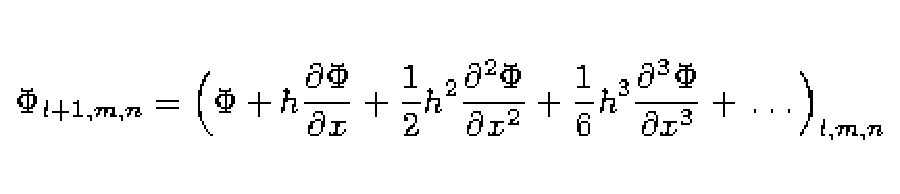
\includegraphics{psfiles/eqn1}}}
 \lower.5\ht 1\box1
\end{equation}
\begin{eqnarray}
 \nonumber
 \setbox1=\hbox{\scalebox{.6}{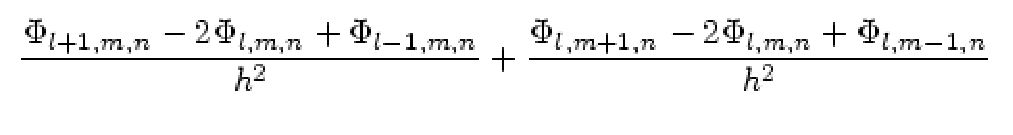
\includegraphics{psfiles/eqarrA1}}}
 \lower.5\ht1 \box1&&\\
 \setbox1=\hbox{\scalebox{.6}{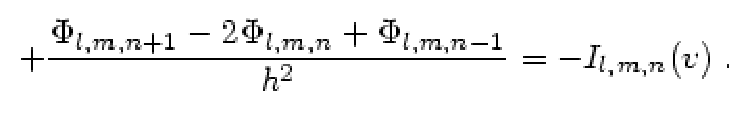
\includegraphics{psfiles/eqarrB1}}}
 \lower.5\ht1 \box1&&
\end{eqnarray}
\end{latexonly}
\caption{Images of equation displays, at normal screen resolution}\label{eq:pics}
\end{figure}

\noindent
These images of the whole environment were created 
using the \Lc{htmlimage} command, to suppress the extended parsing 
that usually occurs when the `\texttt{math}' extension is loaded; viz.
%
%begin{latexonly}
\begin{small}
%end{latexonly}
\begin{verbatim}
\begin{equation}
\htmlimage{no_antialias}
\Phi_{l+1,m,n} = \Bigl(\Phi+h\frac{\partial\Phi}{\partial x} +
...
\end{equation}
%
\begin{eqnarray}
\htmlimage{}
\frac{\Phi_{l+1,m,n}-2\Phi_{l,m,n}+\Phi_{l-1,m,n}}{h^{2}} +
...
\end{eqnarray}
\end{verbatim}
%begin{latexonly}
\end{small}
%end{latexonly}
Further aspects of the options available when generating images 
are discussed in \htmlref{the next section}{imgcon}, in particular 
with regard to the quality of \htmlref{printed images}{printqual}.



\index{mbox@\Lc{mbox} command with math!generates an image}%
\paragraph*{The \Lc{mbox} command.}
Another way to force an image to be created of a mathematical expression,
when global settings are not such as to do this anyway, 
is via the \Lc{mbox} command having math delimiters within its argument.

Normally \Lc{mbox} is used to set a piece of ordinary text within a 
mathematics environment. It is not usual to have math delimiters 
\texttt{\$...\$} or \Lc{(}...\Lc{)} within the argument of an \Lc{mbox}. 
Whereas earlier versions of \latextohtml{} simply ignored the \Lc{mbox} 
command (treating its argument as normal text), 
the presence of such delimiters now results in an image being
generated of the \emph{entire contents} of the \Lc{mbox}.
It is not necessary for there to be any actual mathematics inside
the \Lc{mbox}'s contents;\html{\\}
e.g. \verb|\mbox{...some text...${}$}|
will cause an image to be created of the given text.


\index{parbox@\Lc{parbox} command!generates an image}%
\paragraph*{The \Lc{parbox} command.}
The \Lc{parbox[}\Meta{align}\verb|]{|\Meta{width}\verb|}{|\Meta{text}\verb|}| 
command also generates an image of its contents,
except when used within a \env{tabular} environment, or other
similar table-making environment.
Here the important aspect is the width specified for the given
piece of text, and any special line-breaks or alignments that
this may imply. Hence to get the best effect, \LaTeX{} is used
to typeset the complete \Lc{parbox}, with its specified width,
alignment and contents, resulting in an image.


\index{heqn.sty@\texttt{heqn.sty} style-file}%
\index{package!heqn@\env{heqn}}\index{heqn@\env{heqn} package}%
\index{eqnarray@\env{eqnarray} environment}%
\index{equation@\env{equation} environment}\html{\\}%
\paragraph*{The \env{heqn} package.}
%
If you need \texttt{HTML} 2.0 compatible Web pages,
and have a document with a great many displayed equations, 
then you might try using the \env{heqn} package.  
Inclusion of the \fn{heqn.sty} file has absolutely
no effect on the printed version of the article, 
but it does change the way in which \latextohtml{} translates
displayed equations and equation arrays.  
It causes the equation numbers of the \env{equation}
environment to be moved outside of the images themselves, 
so that they become order-independent and hence recyclable.  
Images that result from the \env{eqnarray} environment are also recyclable,
so long as their equation numbers remain unchanged from the previous run.  

\index{nonumber@\Lc{nonumber}}%
\index{package!html@\env{html}}%
\index{html@\env{html} package}\html{\\}%
The \Lc{nonumber} command is recognised 
in each line of the equation array, to suppress the equation number.
A side-effect of this approach is that equation numbers will
appear on the left side of the page.
The \env{heqn} package requires the \env{html} package.%

\smallskip\noindent
Using \texttt{HTML} Version 3.2 the \env{heqn} package is quite redundant,
since equation numbers are placed in a separate \HTMLtag{TABLE} cell
to the mathematical expressions themselves.
It is \emph{not} required and should \emph{not} be requested, since this will
override some of the improved functionality already available.




\subsection{Figures and Image Conversion\label{imgcon}%
%\section{Figures and Image Conversion\label{imgcon}%
\index{images@images\protect\label{IIIimages}}}%
\tableofchildlinks*\htmlrule
%
\noindent
\latextohtml{} converts equations, special accents, external \PS\ 
files, and \LaTeX{}  environments it cannot directly translate into 
inlined images. This section describes how it is possible to control
the final appearance of such images. For purposes of discussion \dots
\begin{itemize}
\item
``small images'' \index{images!small images}\html{\\}%
refers to inline math expressions, special accents and
any other \LaTeX{} command which causes an image to be generated; while \dots 
\item
``figures'' \index{images!figures}\html{\\}%
applies to image-generating \LaTeX{} environments 
(e.g. \env{makeimage}, \env{figure}, \env{table} (with \texttt{HTML} 2.0), 
 and displayed math environments when required to generate images, etc.).
\end{itemize}

\index{images!math scale-factor}%
\index{images!display scale-factor}%
\index{images!figure scale-factor}%
\index{images!scale-factor, default 1}\html{\\}%
\noindent
These parameters apply only to bitmapped image types,
and have no effect with the default SVG image type.
The size of all ``small images'' depends on a configuration variable
\fn{\$MATH\_SCALE\_FACTOR} which specifies how much to enlarge or 
reduce them in relation to their original size in the \PS\  
version of the document. 
For example a scale-factor of 0.5 will make all images half as big, 
while a scale-factor of 2 will make them twice as big.
Larger scale-factors result in longer processing times and larger 
intermediate image files. A scale-factor will only be effective 
if it is greater than 0. 
The configuration variable \fn{\$FIGURE\_SCALE\_FACTOR} performs
a similar function for ``figures''. 
Both of these variables are initially set to have value 1.

A further variable \fn{\$DISP\_SCALE\_FACTOR} is used with
`displayed math' equations and formulas;
this value multiplies the \fn{\$MATH\_SCALE\_FACTOR} 
to give the actual scaling used.
Values greater than 1 can be used to counteract readability problems
with bitmapped images.
Accordingly this manual actually uses values of 1.4 and 1.2 respectively,
for \fn{\$MATH\_SCALE\_FACTOR} and \fn{\$DISP\_SCALE\_FACTOR}.
These go well with the browser's text-font set at 14\,pt. 
The next larger size of 17\,pt is then used for the \HTMLtag{LARGE} tags
in displayed equations.

\index{images!extra scaling}%
\index{images!improved print quality}%
\index{extra scaling of images}\html{\\}%

A further variable \fn{\$EXTRA\_IMAGE\_SCALE} allows images to be created
at a larger size than intended for display. 
The browser itself scales them down to the intended size, 
but has the extra information available for a better quality print. 
This feature is also available with single images. It is discussed, 
with examples, \hyperref{on the next page}{in Section~}{}{printqual}.


\index{htmlimage@\Lc{htmlimage}}%
\index{html.sty@\texttt{html.sty} style-file}%
\index{figures!fine control}%
\paragraph*{\Lc{htmlimage\char123}\Meta{options}\texttt{\char125}\label{htmlimage}}
%
For finer control, several parameters affecting the conversion 
of a single image can be controlled
with the command \Lc{htmlimage}, which is defined in \fn{html.sty}.
With version \textsc{v97.1} use of this command has been extended to allow
it to control whether an image is generated or not
for some environments,
as well as specifying effects to be used when creating this image.

If an \Lc{htmlimage} command appears within any environment
for which creating an image is a possible strategy (though not usual,
due to loading of extensions, say), then an image will indeed be
created. Any effects requested in the \Meta{options} argument will be used.
Having empty \Meta{options} still causes the image to be generated.

This ability has been used within this manual, for example with the
mathematics images in \hyperref{the previous section}{Figure~}{}{eq:pics}.

\medskip\noindent
The \Meta{options} argument is a string separated by commas.
\index{images!options}\html{\\}% 
Allowable options are:
%
\index{images!scale}%
\index{figures!arbitrarily scaled}%
\begin{itemize}
\item \texttt{scale=}\Meta{scale-factor}\\
allows control over the size of the final image.

\index{images!external}\label{external}%
\index{images!inlined by default}%
\index{images!hypertext link}%
\item \texttt{external}\\
will cause the image not to be inlined; 
instead it will be accessible via a hyperlink. 

\index{thumbnail}\index{images!thumbnail}%
\index{thumbnail!implies external}%
\index{thumbnail!ignores scale-factors}%
\label{thumbnail}%
\item \texttt{thumbnail=}\Meta{scale-factor}\\
will cause a small inlined image to be placed in the caption. 
The size of the thumbnail depends on the \Meta{scale-factor},
as a factor of the `natural size' of the image, ignoring
any \fn{\$FIGURE\_SCALE\_FACTOR} or \fn{\$MATH\_SCALE\_FACTOR}, etc.
which may be applicable to the full-sized version of the image. 
Use of the `\texttt{thumbnail=}' option implies 
the `\texttt{external}' option. 

\index{images!image-map}%
\index{images!server-side image-map}%
%
\item \texttt{map=}\Meta{server-side image-map URL}\\
specifies that the image is to be made into an 
active image-map.
(See \hyperref{another section}{Section~}{}{ImageMaps} for more information.)

\index{images!client-side image-map}\html{\\}%

\item \texttt{usemap=}\Meta{client-side image-map URL}
same as previous item, but with the image-map processed by the client.
(See \hyperref{another section}{Section~}{}{ImageMaps} for more information.)

\index{images!flip option}
\index{figures!oriented}\index{tables!oriented}\html{\\}%

\item \texttt{flip=}\Meta{flip\_option}\\
specifies a change of orientation of the
electronic image relative to the printed version.
The \Meta{flip\_option} is any single command recognised by
the \fn{pnmflip} graphics utility.
The most useful of these include:
\begin{itemize}
%
\item `\texttt{rotate90}' or `\texttt{r90}'~
This will rotate the image clockwise by $90^\circ$.
%
\item `\texttt{rotate270}' or `\texttt{r270}'~
This will rotate the image counterclockwise by $90^\circ$.
%
\item `\texttt{leftright}'~ 
This will flip the image around a vertical axis of rotation.
%
\item `\texttt{topbottom}'~
This will flip the image around a horizontal axis of rotation.
\end{itemize}
%
\index{images!alignment}\index{equations!alignment}%
\index{HTML@\texttt{HTML}!Version 3.0}%
\item \texttt{align=}\Meta{alignment}\\
specifies how the \env{figure} will be aligned.  
The choices are:  
`\texttt{top}', `\texttt{bottom}', `\texttt{middle}', `\texttt{left}', 
`\texttt{right}' and `\texttt{center}'.

The `\texttt{middle}' option specifies that the image is to be
left-justified in the line, but centered vertically.  
The `\texttt{center}' option specifies that it should also 
be centered horizontally. 
This option is valid only if the \texttt{HTML} version 
is \texttt{3.0} or higher.
The default alignment is `\texttt{bottom}'.%

\index{images!transparent}%
\index{transparent images!override defaults}%
%
\item \texttt{transparent}, \texttt{no\_transparent}
 or \texttt{notransparent}\\
specify that a transparent background should (not) be used with this image,
regardless of the normal behaviour for similar images.

\index{images!anti-alias}%
\index{anti-aliasing!override defaults}%
\item \texttt{antialias}, \texttt{no\_antialias}
 or \texttt{noantialias}\\
specify that anti-aliasing should (not) be used with this image,
regardless of the normal behaviour for similar images.

\index{images!extra scaling}%
\item \texttt{extrascale=}\Meta{scale-factor}\\
is used mainly used with a \Meta{scale-factor} of 1.5 or 2, when it is 
important to get printed versions of the completed \texttt{HTML} pages. 
The image is created scaled by the amount specified, but it is embedded 
in the \texttt{HTML} page with attributes to the \HTMLtag{IMG} of
\texttt{HEIGHT=...} and \texttt{WIDTH=...}, 
indicating the \emph{unscaled} size. 
A browser is supposed to display the image at the requested size
by scaling the actual image to fit, 
effectively imposing its own anti-aliasing.
Some examples of this effect are show 
\hyperref{here}{later, in Section~}{}{printqual}.
This effect can be applied to all images in a document by setting
the \fn{\$EXTRA\_IMAGE\_SCALE} \htmlref{variable}{ximagescale}.
However it may be desirable to also turn off ``anti-aliasing''\index{anti-aliasing}, 
as these effects serve similar purposes but need not work well together. 
Furthermore different browsers may give results of different quality.
It may be necessary to experiment a little,
in order to find the combination that works best at your site.

\index{images!specified width or height}%
\item \texttt{height=}\Meta{dimen}\quad
 and\quad\texttt{width=}\Meta{dimen}\\
are used to specify exactly the size to be occupied by the image
on the \texttt{HTML} page. The value(s) given this way overrides
the natural size of the image and forces the browser to shrink or
stretch the image to fit the specified size.
The \Meta{dimen} can be given as either (i) a number (of points);
or (ii) with any of the units of $\mathrm{cm, mm, in, pt}$;
or (iii) fraction of \Lc{hsize} or \Lc{textwidth},
to become a percentage of the browser window's width,
or of \Lc{vsize} or \Lc{textheight} for a percentage height.

\noindent
\textbf{Note:} images whose sizes are modified in this way may not 
be acceptable for 
\hyperref{image-recycling}{image-recycling, (see page~}{)}{recycling}. 
Instead they may need to be generated afresh on each run of \latextohtml{} 
through the same source document.
%
\end{itemize}

\medskip\noindent
In order to be effective the \Lc{htmlimage} command 
and its options must be placed \emph{inside the environment} 
on which it will operate.
Environments for alignment and changing the font size do not
generate images of their contents. Any \Lc{htmlimage}
command may affect the surrounding environment instead;
e.g. within a \env{table} or \env{figure} environment,
but does not apply to a \env{minipage}.

When the \Lc{htmlimage} command occurs in an inappropriate
place, the following message is printed among the warnings
at the end of processing. 
The actual command is shown, with its argument; 
also the environment name and identifying number, if there is one.
%
\begin{quote}
\begin{small}
\begin{verbatim}
The command "\htmlimage" is only effective inside an environment 
which may generate an image (e.g. "{figure}", "{equation}")
 center92: \htmlimage{ ... }
\end{verbatim}
\end{small}
\end{quote}


\subsubsection{An Embedded Image Example\index{images!embedded image}}%
%\subsection{An Embedded Image Example\index{images!embedded image}}%
%
\index{thumbnail}\html{\\}%
The effect of the \LaTeX{}  commands below can be seen in the
\htmlref{thumbnail sketch of Figure}{fig:example} \ref{fig:example}.
A~5\,pt border has also been added around the thumbnail, 
using \Lc{htmlborder} \htmlref{command}{htmlborder}; 
this gives a pseudo-3D effect in some browsers.
%begin{latexonly}
\begin{small}
%end{latexonly}
\begin{verbatim}
\begin{figure}
    \htmlimage{thumbnail=0.5}
    \htmlborder{5}
    \centering 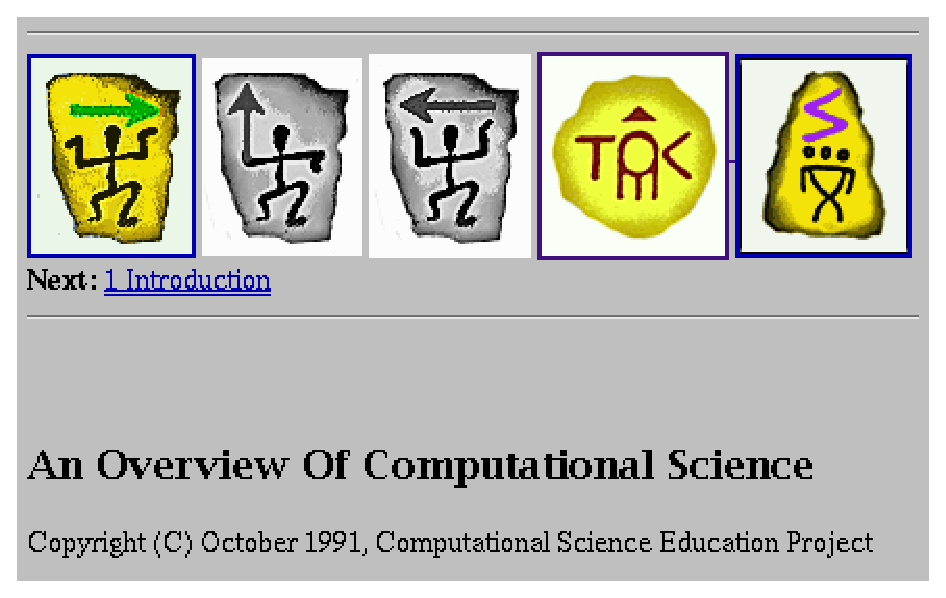
\includegraphics[width=5in]{psfiles/figure}
    \latex{\addtocounter{footnote}{-1}}
    \caption{A sample figure showing part of a page generated by
       \latextohtml{} containing a customised navigation panel 
       (from the 
        CSEP project).}\label{fig:example}
\end{figure}
\end{verbatim}
%begin{latexonly}
\end{small}
%end{latexonly}

\index{figures}%
\index{figure@\env{figure} environment}%
\index{environment!figure@\env{figure}}%
\index{Computer~Science~Education~Project!CSEP}% 
\begin{figure}[hbt]
    \htmlimage{thumbnail=0.5}
    \htmlborder{5}
    \centering 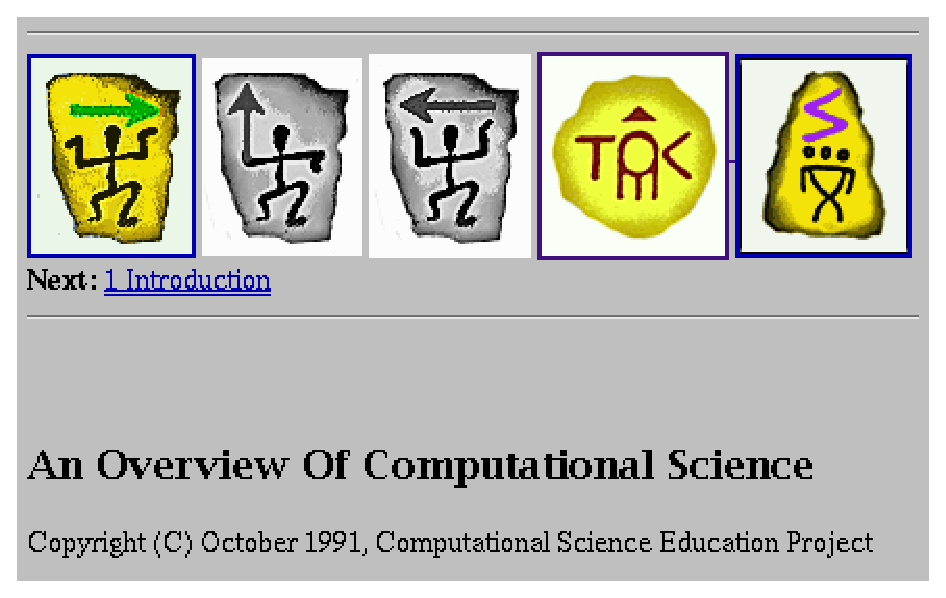
\includegraphics[width=5in]{psfiles/figure}
    \latex{\addtocounter{footnote}{-1}}%
    \caption{A sample figure showing part of a page generated by
       \protect\latextohtml{} containing a customised navigation panel 
       (from the 
        CSEP project).}\label{fig:example}
\end{figure}


\index{htmlimage@\Lc{htmlimage}!overrides configuration}%

\noindent
The \Lc{htmlimage} command is also often useful to cancel-out the
effect of the configuration variable \fn{\$FIGURE\_SCALE\_FACTOR}.
For example to avoid resizing a color screen snap despite 
the value of \fn{\$FIGURE\_SCALE\_FACTOR} it is possible to 
use \verb|\htmlimage{scale=0}|\,.


\subsubsection{Image Sharing and Recycling\label{recycling}}%
%\subsection{Image Sharing and Recycling\label{recycling}}%
\index{images!recycling}\index{images!sharing}%
It is not hard too see how reasonably sized papers,
especially scientific articles, can require
the use of many hundreds of external images.  For this reason,
image sharing and recycling is of critical importance.
In this context, ``sharing'' refers to the use of one
image in more than one place in an article.  ``Recycling''
refers to the use of an image left over from a previous
run of \latextohtml.  Without this ability, every instance of an
image would have to be regenerated each time even the
slightest change were made to the document.

\index{images!thumbnail}\index{thumbnail}%
\index{images!small images}%
\index{images!image-maps}%
\index{images!order-sensitive}%
\index{images!order-insensitive}%
\index{equations!array}%
\index{environment!\env{equation}}\index{environment!eqnarray@\env{eqnarray}}%
\index{eqnarray@\env{eqnarray} environment}\html{\\}%
%
All types of images can be shared.  These include ``small images''
and figures with or without \htmlref{thumbnails}{thumbnail}
and \htmlref{image-maps}{ImageMaps}.
Furthermore, most images can also be reused.  The only
exception are those which are \emph{order-sensitive},
meaning that their content depends upon their location.
Examples of order-sensitive images are \env{equation} 
and \env{eqnarray} environments, 
when \Cs{html\_version 2.0} has been specified;
this is because their figure numbers are part of the image.

\index{figures!captions}%
\index{tables!captions}\html{\\}%

Figures and tables with captions, on the other hand, 
are order-insensitive because the figure numbers 
are not part of the image itself.%
Similarly when \HTMLiii{} code is being produced, equation
numbers are no longer part of the image.
Instead they are placed in a separate cell of a \HTMLtag{TABLE}.
So most images of mathematical formulas can be reused also.%


\subsubsection{Quality of Printed Images\label{printqual}}
%\subsection{Quality of Printed Images\label{printqual}}
%
%% \begin{htmlonly}
Since it is often desirable to get a good quality print on paper
directly from the browser, \hyperref{here are}{Figure~}{ shows}{eq:pics15} 
the same equations as \hyperref[page]{earlier}{on page~}{}{eq:pics}.
This time the `\texttt{extrascale=}' option has been used with a value of 1.5\,.
More than twice the number of pixels are available, 
for a cost of approximately 1.7 times the disk-space\footnote{This figure
varies with the graphics format used, and the complexity of the actual image.}.

%% \end{htmlonly}

\begin{figure}[hb]
%% \begin{htmlonly}
%% \begin{makeimage}
%% \end{makeimage}
%% \begin{equation}
%% \htmlimage{no_antialias,extrascale=1.5}
%% \Phi_{l+1,m,n} = \Bigl(\Phi+h\frac{\partial\Phi}{\partial x} +
%% \frac{1}{2}h^2\frac{\partial^2\Phi}{\partial x^2} +
%% \frac{1}{6}h^3\frac{\partial^3\Phi}{\partial x^3} + \,\ldots\,\Bigr)_{l,m,n}
%% \end{equation}
%% \begin{eqnarray}
%% \htmlimage{extrascale=1.5}
%% \frac{\Phi_{l+1,m,n}-2\Phi_{l,m,n}+\Phi_{l-1,m,n}}{h^{2}} +
%% \frac{\Phi_{l,m+1,n}-2\Phi_{l,m,n}+\Phi_{l,m-1,n}}{h^{2}} \nonumber \\
%% + \frac{\Phi_{l,m,n+1}-2\Phi_{l,m,n}+\Phi_{l,m,n-1}}{h^{2}} = -I_{l,m,n}(v)
%% \end{eqnarray}
%% \end{htmlonly}
%% %
%% \begin{latexonly}
\begin{equation}
 \hbox{\scalebox{.4}{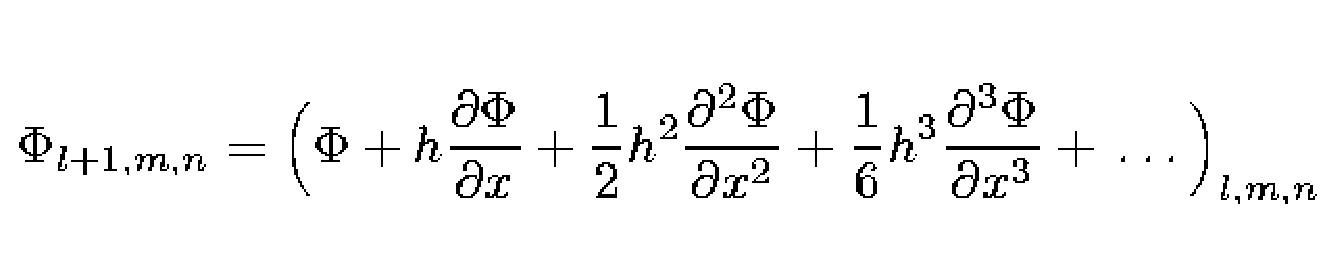
\includegraphics{psfiles/eqn15}}}
\end{equation}%
\begin{eqnarray}
 \nonumber
 \hbox{\scalebox{.4}{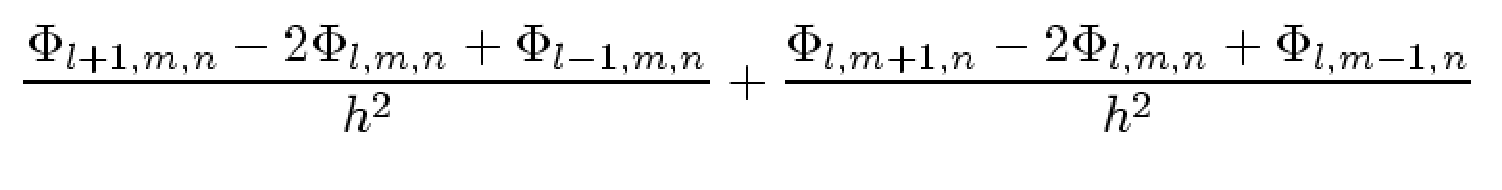
\includegraphics{psfiles/eqarrA15}}}
 &&\\
 \hbox{\scalebox{.4}{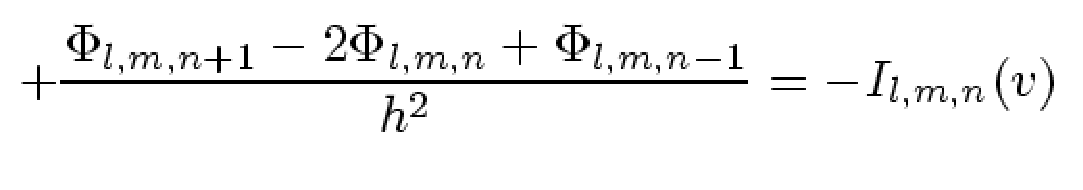
\includegraphics{psfiles/eqarrB15}}}
 &&
\end{eqnarray}
%% \end{latexonly}
\caption{Displayed math environments with \emph{extra-scale} of 1.5}
\label{eq:pics15}%
\end{figure}

%% \begin{latexonly}
\noindent
Since it is often desirable to get a good quality print on paper
directly from the browser, \hyperref{here are}{Figure~}{ shows}{eq:pics15}
the same equations as \hyperref[page]{earlier}{on page~}{}{eq:pics}.
This time the `\texttt{extrascale=1.5}' option has been used. This value of 1.5
means that more than twice the number of pixels are available,
for a cost of approximately 1.7 times the disk-space\footnote{This figure
varies with the graphics format used, and the complexity of the actual image.}.
%% \end{latexonly}
\noindent
On-screen these images appear slightly blurred or indistinct. 
However there can be marked improvement in the print quality,
when printed from some browsers; others may show no improvement at all. 
The ``anti-aliasing'' helps on-screen. In the printed version
jagged edges are indeed softened, but leave an overall fuzziness. 


\hyperref{Here are}{Figure~}{ shows}{eq:pics2} 
the same equations yet again; this time with `\texttt{extrascale=2.0}'.
Now there are 4~times the pixels at a cost of roughly 2.45~times the disk space.
Compared with the previous images (having 1.5~times extra-scaling), 
there is little difference in the on-screen images.
Printing at 300\,dpi shows only a marginal improvement;
but at 600\,dpi the results are most satisfying, especially when
scaled to be comparable with normal 10\,pt type\latex{, as here}.

\begin{figure}[ht]
%% \begin{htmlonly}
%% \begin{makeimage}
%% \end{makeimage}
%% \begin{equation}
%% \htmlimage{no_antialias,extrascale=2}
%% \Phi_{l+1,m,n} = \Bigl(\Phi+h\frac{\partial\Phi}{\partial x} +
%% \frac{1}{2}h^2\frac{\partial^2\Phi}{\partial x^2} +
%% \frac{1}{6}h^3\frac{\partial^3\Phi}{\partial x^3} + \,\ldots\,\Bigr)_{l,m,n}
%% \end{equation}
%% \begin{eqnarray}
%% \htmlimage{extrascale=2}
%% \frac{\Phi_{l+1,m,n}-2\Phi_{l,m,n}+\Phi_{l-1,m,n}}{h^{2}} +
%% \frac{\Phi_{l,m+1,n}-2\Phi_{l,m,n}+\Phi_{l,m-1,n}}{h^{2}} \nonumber \\
%% + \frac{\Phi_{l,m,n+1}-2\Phi_{l,m,n}+\Phi_{l,m,n-1}}{h^{2}} = -I_{l,m,n}(v)\;.
%% \end{eqnarray}
%% \end{htmlonly}
%% %
%% \begin{latexonly}
\begin{equation}
 \setbox1=\hbox{\scalebox{.3}{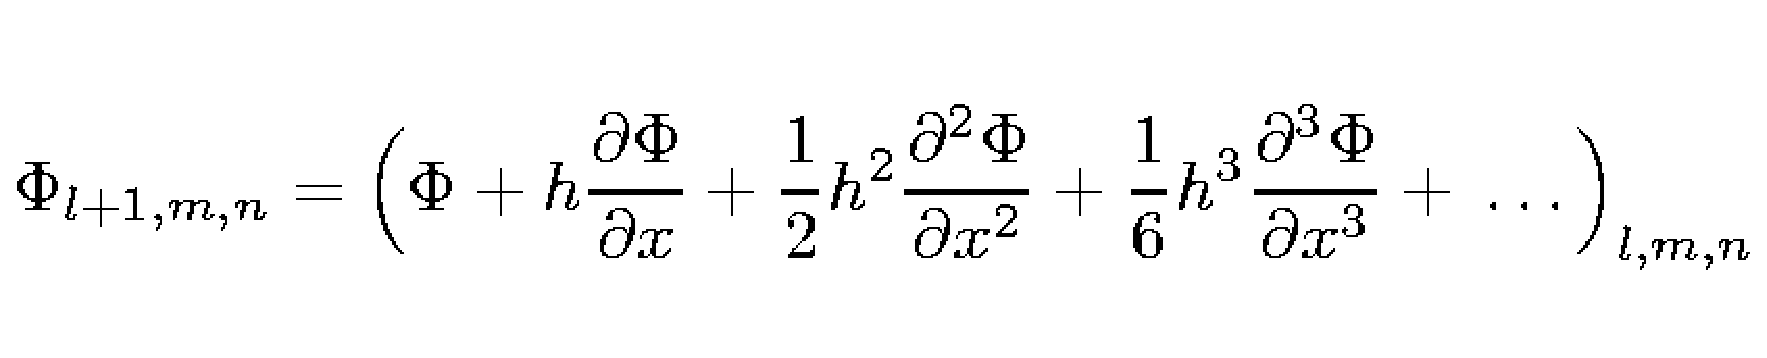
\includegraphics{psfiles/eqn2}}}
 \lower.5\ht1 \box1
\end{equation}
\begin{eqnarray}
 \nonumber
 \setbox1=\hbox{\scalebox{.3}{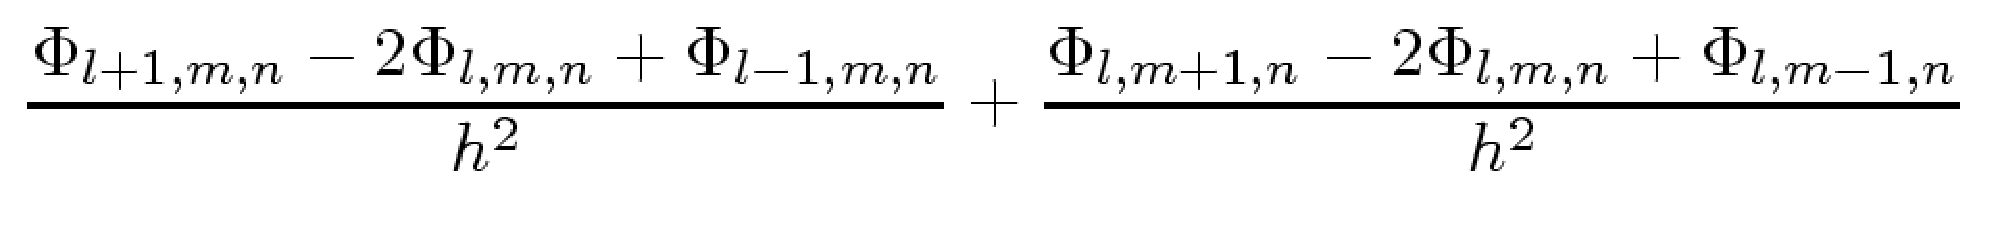
\includegraphics{psfiles/eqarrA2}}}
 \lower.5\ht1 \box1&&\\
 \setbox1=\hbox{\scalebox{.3}{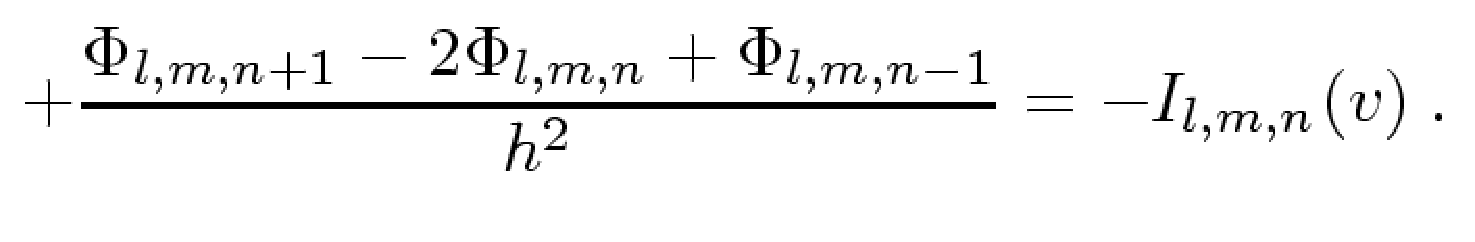
\includegraphics{psfiles/eqarrB2}}}
 \lower.5\ht1 \box1&&
\end{eqnarray}
%% \end{latexonly}
\caption{Displayed math environments with \emph{extra-scale} of 2.0}
\label{eq:pics2}
\end{figure}



\subsection{Figures, Tables and Arbitrary Images\label{sec:figs}}
%\section{Figures, Tables and Arbitrary Images\label{sec:figs}}
\index{tables}%
\index{environment!arbitrary}\index{arbitrary environments}\html{\\}% 
This section is to explain how the translator handles figures, tables
and other environments. 
Compare the paper with the online version.

When the common version of \texttt{HTML} was only 2.0, then almost all
complicated environments were represented using images. However with
\texttt{HTML} 3.2, there is scope for sensible layout of tables,
and proper facilities for associating a caption with a figure or table.
To take advantage of this, the \env{figure} environment now has its
contents placed within \HTMLtag{TABLE} tags; any caption is placed
as its \HTMLtag{CAPTION}.

For consistency with former practice, the contents of the \env{figure}
environment are usually represented by generating an image. 
This is frequently exactly what is required; but not always.
\hyperref[page]{In another section}{On page~}{}{makeimage} it is 
described how to use the \env{makeimage} environment,
defined in the \fn{html.sty} package, to determine just which parts (if any)
of a \env{figure} environment's contents should be made into images,
the remainder being treated as ordinary text, etc.

\medskip
\index{table@\env{table} environment}%
\index{environment!table@\env{table}}\html{\\}%
\paragraph*{\env{table} and \env{tabular} environments.}

Similarly the \env{makeimage} environment can be used within
a \env{table}, though usually this is used with a \env{tabular}
or other table-making environment, such as \env{tabbing} or
\env{longtable} or \env{supertabular}.
Here is a simple example, from the \LaTeX{} \htmlcite{`blue book'}{lamp:latex}.

\begin{table}[hbt]
\begin{center}
\begin{tabular}{||l|lr||}   \hline
gnats   &       gram    &       \$13.65  \\ \cline{2-3}
        &       each    &        .01    \\ \hline
gnu     &       stuffed &        92.50  
                \\  \cline{1-1} \cline{3-3}
emur    &               &       33.33   \\ \hline
armadillo       & frozen        &       8.99 \\ \hline
\end{tabular}
\caption{A sample table taken from \protect\cite{lamp:latex}%}
\index{table@\env{table} environment}%
\index{environment!table@\env{table}}}%
\label{tab}
\end{center}
\end{table}

\begin{htmlonly}
When using \texttt{ -html\_version 2.0} to get code compatible
with the \texttt{HTML} 2.0 standard, an image is made of the
table, as follows:
%
\begin{table}[ht]
\begin{center}
\begin{makeimage}
\begin{tabular}{||l|lr||}   \hline
gnats   &       gram    &       \$13.65  \\ \cline{2-3}
        &       each    &        .01    \\ \hline
gnu     &       stuffed &        92.50  
                \\  \cline{1-1} \cline{3-3}
emur    &               &       33.33   \\ \hline
armadillo       & frozen        &       8.99 \\ \hline
\end{tabular}
\end{makeimage}
\caption{Alternate view of the table from \protect\cite{lamp:latex}}
\label{tab:alt}
\end{center}
\end{table}
\end{htmlonly}
%
%begin{latexonly}
\noindent
Table~\ref{tab:alt} is a screen-shot of how the resulting table appears on-screen,
using a typical browser supporting \HTMLiii.
Here it is scaled down by 70\% to compensate for the 14\,pt fonts being used when
the screen-shot was taken.
%
\begin{table}[ht]
\begin{center}
 \scalebox{.7}{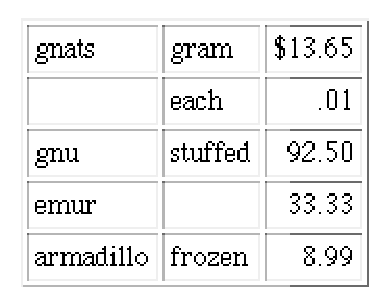
\includegraphics{psfiles/table}}
\caption{Alternate view of the table from \protect\cite{lamp:latex}}
\label{tab:alt}
\end{center}
\end{table}
%end{latexonly}

\medskip
\index{minipage@\env{minipage} environment}%
\index{environment!minipage@\env{minipage}}\html{\\}%
\paragraph*{\env{minipage} environments.}

The special feature of \env{minipage} environments is in the
way \Lc{footnote} and \Lc{footnotemark} commands are handled. 
These are numbered separately from the rest of the footnotes
throughout the document, and the notes themselves are collected together 
to be displayed at the end of the \env{minipage}'s contents.

\medskip
\begin{minipage}{.9\textwidth}
%begin{latexonly}
\renewcommand{\thempfootnote}{\alph{mpfootnote}}
%end{latexonly}
\begin{tabular}{|l|l|} \hline
\textbf{Variable} & \textbf{Meaning} \\ \hline
none      & none                   \\
Jacobi    & $m$-step Jacobi iteration\footnote[1]{one footnote} \\
SSOR      & $m$-step SSOR iteration\footnotemark[1] \\
IC        & Incomplete Cholesky factorization\footnote[2]{another footnote} \\
ILU       & Incomplete LU factorization\footnotemark[2] \\ \hline
\end{tabular}
\end{minipage}

\bigskip\noindent
The code used for this example was as follows\footnote{%
Thanks to John Turner \Email{turner@lanl.gov} for this example, 
which was used in developing
code to handle \env{minipage} environments correctly.}
%begin{latexonly}
\begin{small}
%end{latexonly}
\begin{verbatim}
\begin{minipage}{.9\textwidth}
\renewcommand{\thempfootnote}{\alph{mpfootnote}}
\begin{tabular}{|l|l|} \hline
\textbf{Variable} & \textbf{Meaning} \\ \hline
none      & none                   \\
Jacobi    & $m$-step Jacobi iteration\footnote[1]{one footnote} \\
SSOR      & $m$-step SSOR iteration\footnotemark[1] \\
IC        & Incomplete Cholesky factorization\footnote[2]{another footnote} \\
ILU       & Incomplete LU factorization\footnotemark[2] \\ \hline
\end{tabular}
\end{minipage}
\end{verbatim}
%begin{latexonly}
\end{small}
%end{latexonly}

\bigskip\noindent
\textbf{Warning: }
With some figures, especially when containing graphics imported using
\Lc{includegraphics} or other special macros, the background color
may come out as a shade of grey, rather than white or transparent.
This is due to a setting designed to enhance anti-aliasing of text
within images; e.g. for mathematics.
To alleviate this possible problem, the \Cs{white} command-line option
can be used, to ensure a white background for images of \env{figure}
environments. 
Alternatively, set the \fn{\$WHITE\_BACKGROUND} 
\hyperref{variable}{variable (see section }{)}{cs_white}.


\subsection{Document Classes and Options\label{sec:cls}}
\tableofchildlinks*
\index{document class}%
In general the standard \LaTeX{} document-classes: 
\texttt{article}, \texttt{report}, \texttt{book}, \texttt{letter}, \texttt{slides}
are translated by \latextohtml{} in the same way. 
Currently the only real difference is with the display of section-numbering,
when the \htmlref{\Cs{show\_section\_numbers}}{showsecnums} switch is used,
and when numbering of \htmlref{theorem-like environments}{theoremenvs} 
is linked to section-numbering.

\index{document class!loads file@loads a \texttt{.perl} file}%
\index{document class!options}%

These differences are achieved using a mechanism that automatically loads a file:
\fn{article.perl}, \fn{report.perl}, \fn{book.perl}, \fn{letter.perl}, \fn{slides.perl} 
according to the requested document-class. 
These files contain \Perl{} code and are located in the \fn{styles/} directory.
If a file of the same name exists in the working directory, this will be loaded
instead.

Typically such files \texttt{\Meta{class}.perl} contain code to define subroutines 
or sets values for variables that will affect how certain translations are performed. 
There can be code that is executed only when specific class-options are specified
along with the chosen document-class.
For example, the \fn{foils.perl} implementation of \FoilTeX's \env{foils} class
defines code create a new sub-section for each `foil'.
It also has code which allows \latextohtml{} to ignore those of \FoilTeX's special 
formatting commands that have no relevance when constructing an \texttt{HTML} page.

\medskip 
\index{document class!loads file}%
\index{class-option!loads file}%

Any options given on the \Lc{documentclass} or \Lc{documentstyle} line
may also cause a file containing \Perl{} code to be loaded. 
Such a file is named \texttt{\Meta{option}.perl} for the appropriate \Meta{option}.
When such a file exists, in the local directory or in the \fn{styles/} directory,
it typically contains \Perl{} code to define subroutines or set values for variables 
that will affect how certain translations are performed.
There can be code that is executed only for specific document-classes.

Since the files for class-options are loaded after those for the document-class,
it is possible for the \texttt{\Meta{option}.perl} file to contain code that overrides
settings made within the document-class file.

\medskip\index{class-option!specific file}%
If a file named \texttt{\Meta{class}\_\Meta{option}.perl} happens to exist for
a given combination of document-class \Meta{class} and class-option \Meta{option},
then this will be loaded. 
When such a file exists, reading and executing its contents is done,
rather than executing any \Meta{class}\_\Meta{option} specific information
that may be contained in  \texttt{\Meta{class}.perl} or \texttt{\Meta{option}.perl}~.

\medskip
Currently there are no special option or class-option files provided with 
the \latextohtml{} distribution. It is hoped that users will identify ways 
that specific features can be improved or adapted to specific classes of documents, 
and will write such files themselves, perhaps submitting them for general distribution.

\bigskip
\textbf{Note: }
This mechanism for handling code specific to different document classes
and class-options is more general than that employed by \LaTeXe.
New options can be defined for document-classes generally, or for specific classes,
without the need to have corresponding \texttt{.sty} or \texttt{.clo} files.
\LaTeX{} simply notes the existence of unusupported options---processing is not
interrupted.  



\subsection{Packages and Style-Files\label{sec:sty}}
%\section{Packages and Style-Files\label{sec:sty}}
\tableofchildlinks*
\index{support!for specific style-files}%
\index{support!for german language}\html{\\}%
%
Similar to the document-class mechanism described in
\hyperref{the previous section}{Section}{}{sec:cls},
\latextohtml{} provides a mechanism whereby the code to translate specific
packages and style-files is auto\-matic\-ally loaded, if such code is available.
For example, when use of a style such as \fn{german.sty} 
is detected in a \LaTeX{} source document, either by
\begin{itemize}
\item
a \Lc{usepackage} command of \LaTeXe;
\item
an option to the \Lc{documentstyle} command of \LaTeX\,2.09\,;
\item
an explicit \Lc{input} or \Lc{include} command;
\end{itemize}
the translator looks for a corresponding \texttt{.perl} file
having the same file-name prefix;
e.g. the file \fn{\$LATEX2HTMLDIR/styles/german.perl}.
If such a \texttt{.perl} file is found, 
then its code will be incorporated with the main script,
to be used as required. 

\index{extensions!examples}\html{\\}%

This mechanism helps to keep the core script smaller, as well as making
it easier for others to contribute and share solutions on  
how to translate specific style-files.
The current distribution includes the files to support the styles
listed in \hyperref{the table below}{Table~}{}{styles}.
These provide good examples of how you can create 
further extensions to \latextohtml.%

\index{style-files}\index{packages}%
%\begin{htmlonly}
%\begin{table}
%\end{htmlonly}
\begin{center}
%\begin{tabular}{|c|p{3in}|}
\begin{longtable}{|c|l|}
\caption{Supported \protect\latextohtml\ packages and style-files.}
\\\hline
\endhead
\hline
\endfoot
\label{styles}
\texttt{.perl}~file &\hfill\textbf{Description}\hfill\hfill~\\\hline
\env{\bf alltt}\index{environment!alltt@\env{alltt}}\index{alltt@\env{alltt} environment}%
 & Supports the \LaTeXe's \env{alltt} package.\label{alltt}\\
\env{\bf amsfonts}\index{package!AMSfonts@\env{amsfonts}}\index{AMS@\AmS-\LaTeX!amsfonts@\env{amsfonts} package}%
 & provides recognition of the special \AmS\ font symbols.\label{amsfonts}\\
\env{\bf amsmath}\index{package!AMSmath@\env{amsmath}}\index{AMS@\AmS-\LaTeX!amsmath@\env{amsmath} package}%
 & same as \fn{amstex.perl}.\label{amsmath}\\
\env{\bf amssymb}\index{package!AMSsymb@\env{amssymb}}\index{AMS@\AmS-\LaTeX!amssymb@\env{amssymb} package}%
 & same as \fn{amsfonts.perl}.\label{amssymb}\\
\env{\bf amstex}\index{package!AMStex@\env{amstex}}\index{AMS@\AmS-\LaTeX!amstex@\env{amstex} package}%
 & Supports much of the \AmS-\LaTeX{} package (not yet complete).\label{amstex}\\
\env{\bf babel}\index{package!babel@\env{babel}}\index{babel@\env{babel} package}%
 & Interface to \fn{german.perl} via the \env{babel} package.\label{babel}\\
\env{\bf changebar}\index{package!changebar@\env{changebar}}\index{changebar@\env{changebar} package}%
 & Provides rudimentary change-bar support.\label{changebar}\\
\env{\bf chemsym}\index{package!chemsym@\env{chemsym}}\index{chemsym@\env{chemsym} package}%
 & defines the standard atomic symbols.\label{chemsym}\\
\env{\bf color}\index{package!color@\env{color}}\index{color@\env{color} package}%
 & Causes colored text to be processed as ordinary text by \latextohtml.\label{color}\\
\env{\bf colordvi}\index{package!colordvi@\env{colordvi}}\index{color!colordvi@\env{colordvi} package}%
 & supports the Crayola colors.\label{crayola}\\
\env{\bf enumerate}\index{package!enumerate@\env{enumerate}}\index{enumerate@\env{enumerate} package}%
 & supports structured labels for \env{enumerate} environments.\label{enumerate}\\
\env{\bf epsbox}\index{package!epsbox@\env{epsbox}}\index{epsbox@\env{epsbox} package}%
 & Processes embedded figures not enclosed in a \env{figure} environment.\label{epsbox}\\
\env{\bf epsfig}\index{package!epsfig@\env{epsfig}}\index{epsfig@\env{epsfig} package}%
 & Processes embedded figures not enclosed in a \env{figure} environment.\label{epsfig}\\
\env{\bf finnish}\index{package!finnish@\env{finnish}}\index{finnish!finnish@\env{finnish} package}%
 & Support for the Finnish language.\label{finnish}\\
\env{\bf floatfig}\index{package!floatfig@\env{floatfig}}\index{floatfig@\env{floatfig} package}%
 & Processes floating figures.\label{floatfig}\\
\env{\bf floatflt}\index{package!floatflt@\env{floatflt}}\index{floatflt@\env{floatflt} package}%
 & Processes floating figures and tables.\label{floatflt}\\
\env{\bf foils}\index{class!foils@\env{foils}}\index{foils@\env{foils} class}\index{FoilTeX@\FoilTeX}%
 & Supports \FoilTeX{} system.\label{foils}\\
\env{\bf frames}\index{package!frames@\env{frames}}\index{frames@\env{frames} package}%
 & Provides separate frames for navigation and footnotes.\label{frames}\\
\env{\bf francais}\index{package!francais@\env{francais}}\index{french!francais@\env{francais} package}%
 & Support for the French language, same as \fn{french.perl}.\label{francais}\\
\env{\bf french}\index{package!french@\env{french}}\index{french@\env{french} package}%
 & Support for the French language.\label{french}\\
\env{\bf german}\index{package!german@\env{german}}\index{german@\env{german} package}%
 & Support for the German language.\label{german}\\
\env{\bf germanb}\index{package!germanb@\env{germanb}}\index{german!germanb@\env{germanb} package}%
 & Support for the German language, same as \fn{german.perl}.\label{germanb}\\
\env{\bf graphics}\index{package!graphics@\env{graphics}}\index{graphics@\env{graphics} package}%
 & Supports commands in the \env{graphics} package.\label{graphics}\\
\env{\bf graphicx}\index{package!graphicx@\env{graphicx}}\index{graphics!graphicx@\env{graphicx} package}%
 & Supports the alternate syntax of graphics commands.\label{graphicx}\\
\env{\bf harvard}\index{package!harvard@\env{harvard}}\index{citations!harvard@\env{harvard} package}%
 & Supports the \env{harvard} style of \htmlref{citation}{harvard} (same as fn{nharvard.perl}).\\
\env{\bf heqn}\index{package!heqn@\env{heqn}}\index{heqn@\env{heqn} package}%
 & Alters the way displayed equations are processed.\label{heqn}\\
\env{\bf hthtml}\index{environment!hthtml@\env{hthtml}}\index{hthtml@\env{hthtml} environment}%
 & gives an alternative syntax for specifying hyperlinks, etc.\label{hthtml}\\
\env{\bf htmllist}\index{environment!htmllist@\env{htmllist}}\index{htmllist@\env{htmllist} environment}%
 & Provides support for \htmlref{fancy lists}{htmllist}.\\
\env{\bf justify}\index{package!justify@\env{justify}}\index{justify@\env{justify} package}%
 & supports paragraph alignment---no longer needed.\\
\env{\bf latexsym}\index{package!latexsym@\env{latexsym}}\index{latexsym@\env{latexsym} package}%
 & supports the \LaTeX{} symbol font.\label{latexsym}\\
\env{\bf lgrind}\index{package!lgrind@\env{lgrind}}\index{lgrind@\env{lgrind} package}%
 & macros for nice layout of computer program code.\label{lgrind}\\
\env{\bf longtable}\index{package!longtable@\env{longtable}}%
\index{tables!longtable@longtable\env{longtable} package}%
 & supports use of long tables, as a single table.\label{longtable}\\
\env{\bf makeidx}\index{package!makeidx@\env{makeidx}}\index{makeidx@\env{makeidx} package}%
 & provides more sophisticated indexing.\label{makeidx}\\
\env{\bf multicol}\index{package!multicol@\env{multicol}}\index{columns!multicol@\env{multicol} package}%
 & suppresses requests for multi-columns.\label{multicol}\\
\env{\bf natbib}\index{package!natbib@\env{natbib}}\index{citations!natbib@\env{natbib} package}%
 & Supports many different styles for citations and bibliographies.\label{natbib}\\
\env{\bf nharvard}\index{package!nharvard@\env{nharvard}}\index{citations!nharvard@\env{nharvard} package}%
 & Supports harvard-style citations, using \env{natbib}.\label{nharvard}\\
\env{\bf seminar}\index{package!seminar@\env{seminar}}\index{seminar@\env{seminar} package}%
 & for creation of overhead-presentation slides.\label{seminar}\\
\env{\bf spanish}\index{package!spanish@\env{spanish}}\index{spanish@\env{spanish} package}%
 & Support for the Spanish language.\label{spanish}\\
\env{\bf supertabular}\index{package!supertabular@\env{supertabular}}\index{tables!supertabular@\env{supertabular} package}%
 & supports use super-tables, as an ordinary table.\label{supertabular}\\
\env{\bf texdefs}\index{package!texdefs@\env{texdefs}}\index{texdefs@\env{texdefs} package}%
 & Supports some raw \TeX{} commands.\label{texdefs}\\
\env{\bf verbatim}\index{package!verbatim@\env{verbatim}}\index{verbatim@\env{verbatim} package}%
 & Supports verbatim input of files.\label{verbatim}\\
\env{\bf verbatimfiles}\index{package!verbatimfiles@\env{verbatimfiles}}\index{verbatim!verbatimfiles@\env{verbatimfiles} package}%
 & Supports verbatim input of files, also with line-numbering.\label{verbatimfiles}\\
\env{\bf wrapfig}\index{package!wrapfig@\env{wrapfig}}\index{figures!wrapfig@\env{wrapfig} package}%
 & Supports wrapped figures.\label{wrapfig}\\
\env{\bf xspace}\index{package!xspace@\env{xspace}}\index{xspace@\env{xspace} package}%
 & Supports use of the \env{xspace} package and \Lc{xspace} command.\label{xspace}\\
\env{\bf xy}\index{package!xypic@\protect\Xy-pic}\index{xypic@\protect\Xy-pic package}%
\index{graphics!xy@\protect\Xy-pic package}%
 & Supports use of the \Xy-pic graphics package.\label{xypic}\\
%\hline
\end{longtable}
%\end{tabular}
\end{center}
%\begin{htmlonly}
%\end{table}
%\end{htmlonly}
%\end{table}
\index{extensions!require understanding@require understanding of \Perl{}}\html{\\}%
\noindent
The problem however, is that writing such extensions requires an understanding 
of \Perl{} programming and of the way the processing in \latextohtml{} is organised. 
Interfaces that are more ``user-friendly'' are being investigated.
Some of the techniques currently used are explained in 
\hyperref{a later section}{Section~}{}{sec:ext}.


\subsubsection{Fancy List-Markers\label{htmllist}}
%\subsection{Fancy List-Markers\label{htmllist}}
\index{htmllist@\env{htmllist} environment}%
\index{environment!htmllist@\env{htmllist}}%
%
An optional style-file \fn{htmllist.sty} has been provided which
produces fancier lists in the electronic version of the document%
\html{, }\htmlref{such as this}{listExample}.
This file defines a new \LaTeX{} environment \env{htmllist},
which causes a user-defined item-mark to be placed at each new
item of the list, and which causes the optional description
to be displayed in bold letters.
The filename prefix for the item-mark image can be given as an
optional parameter; see example below. The images distributed with
\latextohtml{} for this purpose are listed with the description
of the \verb|\htmlitemmark| command, which provides an alternative
means of choosing the item-mark, and allows the image to be changed
for different items in the list.

\index{htmlitemmark@\Lc{htmlitemmark}}%
\index{htmllist@\env{htmllist}!prints as@prints as \env{description}}%
\index{htmllist@\env{htmllist}!item-marks}%
\index{environment!htmllist@\env{htmllist}}\html{\\}%
%
The mark is determined
by the \verb|\htmlitemmark{|\Meta{item-mark}\verb|}| command.  
This command accepts either a mnemonic name for the \Meta{item-mark}, 
from a list of icons established at installation, or the URL of a mark
not in the installation list. 
The command \Lc{htmlitemmark} must be used \emph{inside} the 
\env{htmllist} environment in order to be effective, 
and it may be used more than once to change the mark within the list.  
The item-marks supplied with \latextohtml{} are 
\texttt{BlueBall}, \texttt{RedBall}, \texttt{OrangeBall}, \texttt{GreenBall}, 
\texttt{PinkBall}, \texttt{PurpleBall}, \texttt{WhiteBall} and \texttt{YellowBall}.
The \env{htmllist} environment is identical to 
the \env{description} environment in the printed version.

\index{htmllist@\env{htmllist}!example}%

\noindent 
An example of its usage is:
%begin{latexonly}
\begin{small}
%end{latexonly}
\begin{verbatim}
\begin{htmllist}[WhiteBall]
\item[Item 1:] This will have a white ball.
\item[Item 2:] This will also have a white ball.
\htmlitemmark{RedBall}%
\item[Item 3:] This will have a red ball.
\end{htmllist}
\end{verbatim}
%begin{latexonly}
\end{small}
%end{latexonly}

\noindent This will produce:\label{listExample}
\begin{htmllist}[WhiteBall]
%begin{latexonly}
\addtolength{\leftskip}{15pt}
%end{latexonly}
\item[Item 1:] This will have a white ball.
\item[Item 2:] This will also have a white ball.
\htmlitemmark{RedBall}%
\item[Item 3:] This will have a red ball.
\end{htmllist}

\index{floatfig@\env{floatingfigure} environment}%
\index{wrapfig@\env{wrapfigure} environment}%
\index{environment!floatingfigure@\env{floatingfigure}}%
\index{environment!wrapfigure@\env{wrapfigure}}\html{\\}%
\noindent
One can also obtain \LaTeXe\ style-files \fn{floatfig.sty} and 
\fn{wrapfig.sty}, which provide support for the \env{floatingfigure}
and \env{wrapfigure} environments, respectively.  These environments
allow text to wrap around a figure in the printed version, 
but are treated exactly as an ordinary \env{figure}s in the electronic version.  
They are described in \hypercite{The \LaTeX{} Companion}%
{\emph{The \LaTeX{} Companion}}{}{goossens:latex}.%

\subsubsection{Support for \FoilTeX\label{sec:foils}}
\index{foils@\env{foils} class}%
\index{FoilTeX@\FoilTeX} The \FoilTeX{} system presents some
additional problems for \latextohtml:
\begin{itemize}
\item It has additional commands like \Lc{foilhead} and
  \Lc{rotatefoilhead}, that roughly correspond to sectioning commands,
\item The images are produced at the sizes suitable for large screen
  presentation, but not for the HTML.
\end{itemize}
The package \fn{foils.perl} deals with these problems. It treats foils as
starred subsections and ignores \FoilTeX-specific commands that have no
meaning for HTML, like \Lc{LogoOn}. The header
\Lc{documentclass[}+\texttt{\it options}\verb+]{foils}+ in the
\fn{images.tex} file is substituted by the header
\Lc{documentclass[}\fn{\$FOILOPTIONS}\verb+]{+\fn{\$FOILCLASS}\verb+}+,
where the variables \fn{\$FOILOPTIONS} and \fn{\$FOILCLASS} can be set
in the configuration file (by default they are \texttt{'10pt'} and
\texttt{'article'} correspondingly).
A further variable \fn{\$FOILHEADLEVEL} holds the level of sectioning
at which a `foil' is to correspond; the default level is 4 (sub-section).

The \LaTeX{} style file \fn{foilhtml.sty} in the \fn{texinputs/}
directory provides some additional features for \FoilTeX{}. It implements
structural markup commands like \Lc{section},
\Lc{tableofcontents} for foils. See the directory \fn{docs/foilhtml/} for
the details.



\subsubsection{Indicating Differences between Document Versions\index{change-bars}}%
%\subsection{Indicating Differences between Document Versions\index{change-bars}}%
\latextohtml{} supports the \LaTeXe\ \fn{changebar.sty} package,
written by Johannes Braams \Email{JLBraams@cistron.nl}, for 
inserting \emph{change-bars} in a document in order to indicate 
differences from previous versions. This is a very primitive form of 
version control and there is much scope for improvement.

\index{change-bars!different versions}% 
Within the \LaTeX{} version of this manual two thicknesses of change-bar 
have been used. Thicker bars indicate changes introduced with version \textsc{v97.1}\,,
while thinner bars indicate earlier additions since \textsc{v96.1}\,.\html{\\}
Within the \texttt{HTML} version the change-bars clearly indicate the 
different revisions with explicit numbering.%
Within the \texttt{HTML} version, the graphic icons representing
the changebars can be followed by some text indicating the new version.
This is used repeatedly throughout\latex{ the online version of}
this manual. It is achieved using the command 
\verb|\cbversion{|\Meta{version}\verb|}|, immediately following
the \verb|\begin{changebar}|. 
This sets a variable \fn{\$cb\_version} to be used both at the beginning
and end of the environment. The value of this variable is retained,
to be used with other \env{changebar} environments, unless changed explicitly
by another occurrence of \fn{\$cb\_version}.

\smallskip\noindent
\textbf{Warning: }
\latextohtml{} will not correctly process \env{changebar} environments
that contain sectioning commands, even when the (sub)sections or
(sub)paragraphs are to occur on the same \texttt{HTML} page.
If this is required, use a separate \env{changebar} environment
within each (sub)section or (sub)paragraph.




\subsection{Indexing\label{index}\index{index|(}}%
%\section{Indexing\label{index}\index{index|(}}%
\index{index!section-names}%
\latextohtml{} automatically produces an Index consisting of the
arguments to all \Lc{index} commands encountered, if there are any.
A hyperlink is created to that point in the text where the 
\Lc{index} command occurred.

More sophisticated indexing is available by loading the \env{makeidx} package.
Most of the features described in \cite[Appendix~A]{lamp:latex} become available.
This includes:
%
\begin{htmllist}\htmlitemmark{RedBall}%
\index{index!styled entries}%
\item 
[styled entries, using `\texttt{@}' : ]
Entries of the form \verb|\index{|\Meta{sort-key}\verb|@|\Meta{styled-text}\verb|}|
produce \Meta{styled-text} as the entry, but sorted according to \Meta{sort-key}.

\index{index!hierarchical}%
\item 
[hierarchical entries, using `\texttt{!}' : ] 
Entries of the form
\verb|\index{|\Meta{item}\verb|!|\Meta{sub-item}\verb|}|
set the \Meta{sub-item} indented below the \Meta{item}.
Unlimited levels of hierarchy are possible, 
even though \LaTeX{} is limited to only 3 levels. 
The \Meta{sort-key}\verb|@|\Meta{styled-text} can be used at each level.

\index{index!page-ranges}%
\item 
[explicit ranges, using `\texttt{|(}' and `\texttt{|)}' : ]
This is perhaps more useful in the \LaTeX{} version. 
In the \texttt{HTML} version these simply insert words ``from'' and ``to'',
respectively, prior to the hyperlink to where the index-entry occurs.

\index{index!cross-link}%
\index{index!see@\texttt{\char124see}}%
\item 
[\texttt{|see\char123}\Meta{index-entry}\texttt{\char125} : ]
provides a textual reference to another indexed word or phrase, 
by inserting the word ``see''. 
This can be used in conjunction with \Lc{htmlref} to create a hyperlink
to the \Meta{index-entry}; viz.
\begin{verbatim}
\index{latexe@\LaTeXe |see{\htmlref{\LaTeX}{IIIlatex}}}
\end{verbatim}
where a \Lc{label} has been specified in some other index-entry, as follows:
\begin{verbatim}
\index{latex@\LaTeX\label{IIIlatex}}
\end{verbatim}

\index{index!emph@\texttt{\char124emph}}%
\item [\texttt{|emph} : ]
\strikeout{is recognised but \emph{ignored}; 
other \texttt{|\Meta{command}} commands are \emph{not} processed by \latextohtml{},
with the following exception\dots} is handled correctly, by applying
\Lc{emph} to the text of the generated hyperlink.

\index{index!style@\texttt{\char124}\Meta{style}}%
\item [\texttt{|}\Meta{style} : ]
where \Meta{style} is the name of \LaTeX{} style-changing command, 
without the initial `\Lc{}'; e.g. `\texttt{emph}', `\texttt{textbf}',
`\texttt{textit}', etc. The corresponding \LaTeX{} command is applied
to the text of the generated hyperlink.

\index{index!blank lines}%
\index{index!alphabetization}%
\item [blank lines and alphabetization: ]
Having precisely a single space-character after the \verb+|+ 
(e.g. \verb+\index{A| }+) 
places a blank line before the index entry and omits the hyperlink.
This is used mainly for visual formatting; it allows a break before the entries
starting with each letter, say. Using a printable-key, as in \verb+\index{Q@Q, R| }+,
is appropriate when there are no indexed words starting with `Q', say.

\index{index!quoted delimiters}%
\item [quoted delimiters: ]
The three special delimiters can be used within the printable portion,
if preceded by the double-quote character: \verb+"@+, \verb+"|+, \verb+"!+ 
and also \verb+""+ for the quote character itself. 
Also \verb|\"| produces an umlaut accent on the following character, 
when appropriate, else is ignored.
%
\end{htmllist}%

\index{index!cross-link}%
\index{index!labelled entries}\html{\\}\noindent
%
Furthermore, the printable part of an index entry can contain \texttt{HTML}
anchors; that is, hyperlinks and/or \verb|\label{...}|s.
This allows index entries to contain cross-links to other entries, for example,
as well as allowing index-entries to be the target of hyperlinks from elsewhere
within the document. 

The \htmlref{next section}{glossind} describes how this feature is used within this
manual to create a Glossary, containing a short description of all file-names,
configuration-variables and application software mentioned within the manual,
integrated with the Index. All occurrences of the technical names can be
easily found, starting from any other.

\index{index!labelled entries}

When a single item is indexed many times, it is sufficient 
to have a \Lc{label} command appearing within the printable portion 
of the first instance of an \verb|\index{...}| command for that item,
within a single document segment. 

\medskip

If the index-entries are in different segments of a segmented document, 
it is sufficient to have the  \verb|\index{...@...\label{...}}| appearing 
within that segment, in which the item is indexed, whose indexing information 
is loaded earliest via a \verb|\internal[index]{...}| command.
When in doubt, include one \verb|\index{...@...\label{...}}| per segment 
in which the item is indexed.

\index{index!cross-link}%
\index{index!cross-link incorrect}

For cross-links to work effectively within segmented documents,
the indexing command 
\verb|\index{...@...\label{...}}| \emph{must} occur earlier 
in the same segment than any use of 
\verb|\index{...@...\htmlref{...}{...}}| 
intended to create a link to that label. 
If the \Lc{label} occurs in a different segment,
then a \verb|\internal[index]{...}| command for that segment,
may be needed at the beginning of the segment with the \Lc{htmlref}\,.
When this is done incorrectly, the resulting link will be to the
segment where the indexed item occurred, 
rather than staying within the Index.

\htmlrule
\index{index!section-names}%
\index{index!cumbersome}%

\noindent
Since use of section-names, as the text for hyperlinks, can lead to a very long
and cumbersome Index, especially when single items have been indexed many times,
a further feature is provided to obtain a more compact Index.
 
\index{index!codified links}\html{\\}%
Use of the command-line option \Cs{short\_index} causes a codified 
representation of the sectioning to be used, rather than the full section-name.
The differences are as follows.
%
\begin{itemize}
%
\item
For example, `\texttt{2.1}' means sub-node~\#1 of node~\#2, 
viewing the entire document as a tree-like structure. 

\index{index!codified links!top-most node}%
\item
The top-most node is simply denoted `\verb|^|'.

\index{segmentation!child-links}%
\index{segmentation!codified index}%
\item
With a \htmlref{segmented document}{Segmentation}, 
each segment is codified separately 
using the \htmlref{\Meta{prefix}}{prefix} supplied for that segment.
The Index includes a legend of these prefixes, 
each giving the title of the leading page from the segment,
as a hyperlink to the place on that page where its 
child-links are displayed.

\index{index!codified links!for easier browsing}%
\item
Hyperlinks start on the same line as the index-key, 
rather than the next line, separated by `\texttt{|}'. 
This gives further compactification for easier browsing.

\index{index!with prefix@with \Meta{prefix}}%
\item
If \Cs{prefix \Meta{prefix}} has been specified, then the \Meta{prefix}
is prepended to the codified form. This is most useful for segmented documents. 
Now the top-most node is indicated by the bare \Meta{prefix}.
\end{itemize}
%
These features can also be obtained by setting the variable \fn{\$SHORT\_INDEX}
to have value `\texttt{1}', in a configuration or initialisation file;
provided, of course, that the document loads the \env{makeidx} package.%

\latex{\index{index|)}}



\subsubsection{Integrated Glossary and Index\label{glossind}}%
%\subsection{Integrated Glossary and Index\label{glossind}}%
\index{index!integrated with Glossary}%
\index{Glossary!integrated with Index}%

\noindent
A large number of different pieces of software are required to make
\latextohtml{} work effectively, as well as many files containing data or code 
to work with parts of this software. 
For this reason, a Glossary is included with this manual. 
It contains the names of all files, configuration variables, application software
and related technical terms, with a short description of what it is, or does,
and perhaps a URL for further reference. 

\index{Glossary!printed version}%
\index{Glossary!HTML@\texttt{HTML} version}\html{\\}%
In the printed version each item in the Glossary is accompanied by the page-numbers
on which the item is mentioned, somewhat like in the Index. 
For the \texttt{HTML} version, each glossary-item contains a hyperlink to an
index-entry, which then has links to each occurrence.
These extra index-entries do not appear in the printed version; 
indeed they also contain a hyperlink back to the corresponding glossary-entry. 

This feature is currently available only when using the \env{makeidx} package,
and needs also the \env{html} and \env{htmllist} packages.
It was developed for version 96.1f by Ross Moore,
incorporating an extensive revision of \fn{makeidx.perl}, as well as additions to
\latextohtml{} so that all aspects of indexing work correctly with segmented documents.

\bigskip
\noindent
Since \LaTeX{} provides no guidelines for how a Glossary should be constructed,
the technique used here will be explained in detail, for both the printed and
\texttt{HTML} versions. 

\begin{itemize}
\item
Firstly the \Lc{makeglossary} command, which is similar to \Lc{makeindex},
must appear in the document preamble, so that \LaTeX{} will record
uses of the \verb|\glossary{...}| command within a file \fn{manual.glo}.

This command is redundant in the \texttt{HTML} version, so is given a trivial
definition which is ignored by \LaTeX{}.\par

\item
Next, the words, phrases or technical terms to be included in the Glossary
are marked in the main text using the \Lc{glossary} command, used indirectly
via other macros. For example, file-names are inserted via 
\verb|\|\verb|fn{html.sty}|, \verb|\|\verb|fn{dvips}|,  \verb|\|\verb|appl{dvips}| etc. 
which both insert the text and create the glossary-entry; \textit{viz.}
%
%begin{latexonly}
\begin{small}
%end{latexonly}
\begin{verbatim}
\newcommand{\fn}[1]{\htmlref{\texttt{#1}}{GGG#1}\glossary{#1}}
\newcommand{\appl}[1]{\htmlref{\textsl{#1}}{GGG#1}%
  \Glossary{#1}{\textsl{#1}}}
\end{verbatim}
%begin{latexonly}
\end{small}
%end{latexonly}

\item
The expansions of \Lc{glossary}, and the slightly more general 
\Lc{Glossary}, are different for the printed and \texttt{HTML} versions.
For the \texttt{HTML} version the following definitions occur 
within an \env{htmlonly} environment:
%
%begin{latexonly}
\begin{small}
%end{latexonly}
\begin{verbatim}
\def\glossary#1{\index{#1@\texttt{#1} \label{III#1}%
  \htmlref{(G)}{GGG#1}}}
\def\Glossary#1#2{\index{#1@{#2} \label{III#1}\htmlref{(G)}{GGG#1}}}
\def\makeglossary{}
\end{verbatim}
%begin{latexonly}
\end{small}
%end{latexonly}
%
\dots while in \LaTeX{} we need only:\quad
\verb|\newcommand\Glossary[2]{\glossary{#1@#2}}|~.

Notice how the feature of \env{makeidx}, allowing the printable portion to
be separate from the sorting-key, is used to allow text-styles to be included within
both index-entries and glossary-entries. Indeed the purpose of \Lc{Glossary} is
to allow deviations from a fixed style, e.g. 
%
%begin{latexonly}
\begin{small}
%end{latexonly}
\begin{verbatim}
\newcommand{\MF}{\htmlref{\textsl{Metafont}}{GGGmetafont}%
  \Glossary{metafont}{\textsl{Metafont}}}%
\end{verbatim}
%begin{latexonly}
\end{small}
%end{latexonly}
%
Also notice that in the \texttt{HTML} version an index-entry is created that
includes, within its printable portion, both a \Lc{label} and a hyperlink.
The former, having name \texttt{III...}, will ultimately reside on the Index page, 
while the latter will point to an anchor named \texttt{GGG...} on the Glossary page.
These names must be distinct from any other names used with \Lc{label}s 
elsewhere in the document, hence the use of prefixes \texttt{III} and \texttt{GGG}.
A short string `\texttt{(G)}' is used for the text of the hyperlink in the Index.

\item
The text descriptions of the glossary-items are stored in a file 
called \fn{l2hfiles.dat}, with one description per line.
For the \texttt{HTML} version this file is actually read as input:
%
\begin{comment}
\begin{small}
\latex{\hskip15pt}\verb|\|\verb|begin{htmlonly}|%
\latex{\vskip-1.1\baselineskip\vskip-1.1\baselineskip\indentverb{15pt}}%
\begin{verbatim}
\section*{Glossary of variables and file-names\label{Glossary}}
\begin{htmllist}\htmlitemmark{OrangeBall}
\input l2hfiles.dat
\end{htmllist}
\end{verbatim}
\latex{\nobreak\vskip-1.1\baselineskip\nobreak\leavevmode\hskip15pt}%
\verb|\|\verb|end{htmlonly}|%
\end{small}%
\end{comment}
%
%begin{latexonly}
\begin{small}
%end{latexonly}
\begin{verbatim}
\section*{Glossary of variables and file-names\label{Glossary}}
\begin{htmllist}\htmlitemmark{OrangeBall}
  \input l2hfiles.dat
\end{htmllist}
\end{verbatim}
%begin{latexonly}
\end{small}%
%end{latexonly}

\noindent
For this reason alone it is desirable to have \fn{l2hfiles.dat} sorted alphabetically.\par

\item
The mechanism used for the \LaTeX{} version also requires the file to be sorted
strictly alphabetically, according to the sort-keys associated to each glossary entry.
\newline
(This requirement could be relaxed, but only with a loss in efficiency; see below.)

\LaTeX{} constructs its Glossary by running the \fn{makeindex} utility 
on the file \fn{manual.glo}, using the following command:
%
%begin{latexonly}
\begin{small}%
%end{latexonly}
\begin{verbatim}
makeindex -o manual.gls -s l2hglo.ist manual.glo
\end{verbatim}
%begin{latexonly}
\end{small}%
%end{latexonly}
%
Its output, which includes page numbering for an index, is stored in \fn{manual.gls}
and subsequently read by \LaTeX{} using:

%begin{latexonly}
\begin{small}%
%end{latexonly}
\begin{verbatim}
\InputIfFileExists{manual.gls}{\clearpage\typeout{^^Jcreating Glossary...}}
{\typeout{^^JNo Glossary, since  manual.gls  could not be found.^^J}}
\end{verbatim}%
%begin{latexonly}
\end{small}%
%end{latexonly}

\noindent
The configuration file \fn{l2hglo.ist} is included along with this manual.
It contains a portion that inserts tricky \TeX{} code at the beginning of \fn{manual.gls}.
This code extracts from \fn{l2hfiles.dat} that line corresponding to each glossary entry, 
then typesets it itemized within an environment called \env{theglossary}.

%begin{latexonly}
\begin{small}%
%end{latexonly}
\begin{verbatim}
\newenvironment{theglossary}{\begin{list}{}{%
  \setlength{\labelwidth}{20pt}%
  \setlength{\leftmargin}{\labelwidth}%
  \setlength\itemindent{-\labelwidth}%
  \setlength\itemsep{0pt}\setlength\parsep{0pt}%
  \rmfamily}}{\end{list}}
\end{verbatim}
%begin{latexonly}
\end{small}%
%end{latexonly}
%
Currently searching within \fn{l2hfiles.dat} is only done sequentially, stopping
at the end of the file. If an entry is not found then it is skipped and a message
printed to the log; the next entry will search from the top of the file.
If all entries are included and maintained in strict order, there will be no skipping 
and each line of \fn{l2hfiles.dat} is read exactly once.\par

\item
Within \fn{l2hfiles.dat} the data lines look like:
%
%begin{latexonly}
\begin{small}%
%end{latexonly}
\begin{verbatim}
\item[\gn{french.perl}] adds \Perl{} code to be compatible with the ...
\item[\gn{\textsl  {ftp}}] `File Transfer Protocols', network ...
\item[\gn{german.perl}] adds \Perl{} code to be compatible with the ...
...
\end{verbatim}
%begin{latexonly}
\end{small}%
%end{latexonly}
%
For the \LaTeX{} version the \verb|\item[\gn{...}]| is only used for pattern-matching, 
to find the correct data entry.
All typesetting is controlled from within \fn{manual.gls}.

However the \texttt{HTML} version requires the following definition:
%
%begin{latexonly}
\begin{small}%
%end{latexonly}
\begin{verbatim}
\newcommand{\gn}[1]{\texttt{#1}\label{GGG#1}\htmlref{\^}{III#1}}%  
\end{verbatim}
%begin{latexonly}
\end{small}%
%end{latexonly}
%
which establishes the hyperlink to the Index, marked by `\verb|^|', 
and provides the \Lc{label} to create the target in the Glossary 
for any \verb|\glossary{...}| command having the corresponding argument.%
\end{itemize}

\section{Hypertext Extensions to \LaTeX}
\label{sec:hyp}\index{special}
\index{hypertext!extensions}\index{extensions!hypertext}

\noindent
This {section} describes how you can define hypertext 
entries in your \texttt{HTML} documents from within your \LaTeX{} source,
as well as other effects available in \texttt{HTML} for which
there need be no direct \LaTeX{} analog for a printed document.
These are implemented as new \LaTeX{} commands which have special 
meaning during the translation by \latextohtml\ into \texttt{HTML}, 
but are mostly ignored when processed by \LaTeX.

\index{html.sty@\texttt{html.sty} style-file}%
\index{html.sty@\texttt{html.sty} package!how to load it}\html{\\}%
The new commands described in the sections 
below are defined mainly in the \env{html} package,
with \LaTeX{} definitions in the file \fn{html.sty},
which is part of the \latextohtml{} distribution. 
It \emph{must be included} in any \LaTeX{} document using these features, 
by one of the following methods:

\begin{itemize}%
\item including \texttt{html} as an optional argument 
to \Lc{documentstyle} in \LaTeX\,2.09\,;
\item including \texttt{html} in a \LaTeXe{} \Lc{usepackage} command.
\end{itemize}

\noindent
It is \emph{not sufficient} to load the style file via an \Lc{input} or
\Lc{include} command, such as \Lc{input}\verb| html.sty|\,.
This will load the required definitions for \LaTeX, but will not load
the \fn{html.perl} package file for \latextohtml.

\smallskip\noindent
\textbf{Warning: } Some of these features, but not all, are also available
with \LaTeX{}\,2.09.\html{\\}
Users of \latextohtml{} are strongly advised to upgrade
their \LaTeX{} installations to \LaTeXe{}. 

\bigskip
\htmlrule[width=300]
\index{conditional text!HTML or@\texttt{HTML} or \LaTeX{} version}\html{\\}%
\noindent
Several new environments are defined, in particular for specifying
large (or small) sections of the text which are appropriate to only
one version of the document---either 
the \texttt{HTML} or the \LaTeX{} typeset version.
\begin{latexonly}
Their use is discussed in Sections \ref{sec:markup} and \ref{sec:latexonly}.
\end{latexonly}
%
\index{html.sty@\texttt{html.sty}!new environments defined}\label{htmlenvs}%
\begin{htmllist}\htmlitemmark{GreenBall}
%
\item[\htmlref{\Lc{begin\char123rawhtml\char125}}{rawhtml}]
for including raw \texttt{HTML} tags and \texttt{SGML}-like markup.
%
\item[\htmlref{\Lc{begin\char123htmlonly\char125}}{htmlonly}]
for material intended for the \texttt{HTML} pages only.
%
\item[\htmlref{\Lc{begin\char123latexonly\char125}}{latexonly}]
for material intended for the \LaTeX{} version only.\html{\\}
Note that any macro-definitions or changes to counter-values are local
to within this environment.
%
\item[\htmlref{\texttt{\%begin\char123latexonly\char125}}{unlatexonly}]
for material intended for the \LaTeX{} version only.\html{\\}
Macro-definitions and changes to counter-values are retained
outside of this (pseudo-)environment.
%
\item[\htmlref{\Lc{begin\char123imagesonly\char125}}{imagesonly}]
for material intended to be used in the \fn{images.tex} file  only.
%
\item[\htmlref{\Lc{begin\char123comment\char125}}{comment}]
for user-comments only, currently ignored in both the \texttt{HTML} 
and \LaTeX{} versions.\html{\\}
(To put \texttt{HTML} comments into the \texttt{HTML} files,
use the \env{rawhtml} environment.)
%
\item[\htmlref{\Lc{begin\char123makeimage\char125}}{makeimage}]%
creates an image of its contents, as typeset by \LaTeX.\html{\\}
This is also used to prevent an image being made of the complete
contents of a \env{figure} environment, allowing more natural processing.
%
\item[\htmlref{\Lc{begin\char123htmllist\char125}}{htmllist}]%
defined in \fn{htmllist.sty} and \fn{htmllist.perl}, 
this produces coloured balls tagging the items in a descriptive list, 
as used throughout\latex{ the \texttt{HTML} version of} this manual.
%
\end{htmllist}
\smallskip\noindent
\textbf{Warning: \label{env:warn}}
When using these environments it is important
that the closing delimiter, \Lc{end}\verb|{htmlonly}| say, occurs
on a line by itself with no preceding spaces, \Meta{tab}s 
or any other characters. 
(Otherwise \LaTeX{} will \emph{not} recognise the intended end 
of the environment when processing for the \texttt{.dvi} version.)
Similarly there should be nothing on the same line \emph{after}
the opening environment delimiter, \Lc{begin}\verb|{htmlonly}| say.

\medskip
\htmlrule[width=300]
\medskip\noindent
The following commands are defined for \LaTeX{} in \fn{html.sty}.\html{\\}
Corresponding \Perl{} implementations are either in \fn{html.perl} 
or in the \fn{latex2html} script itself.
%
\index{hypertext links!commands to create}%
\index{html.sty@\texttt{html.sty}!new commands defined}%
\begin{htmllist}\htmlitemmark{OrangeBall}
%
\item[\htmlref{\Lc{latextohtml}}{l2hname}]
expands to the name \latextohtml, of this translator;
%
\item[\htmlref{\Lc{htmladdnormallink}}{addnormlink}]
creates a (perhaps named) textual hyperlink to a specified \Meta{URL};
%
\item[\htmlref{\Lc{htmladdnormallinkfoot}}{addfootlink}]
same as \Lc{htmladdnormallink}, but \LaTeX{} also prints the \Meta{URL} in a footnote;
%
\item[\htmlref{\Lc{htmladdimg}}{htmladdimg}]
places an image  (perhaps aligned) on the \texttt{HTML} page;\html{\\}
ignored by \LaTeX.
%
\item[\htmlref{\Lc{hyperref}}{hyperref}]
creates a textual hyperlink to where a \Lc{label} command 
occurred within the same document.\html{\\}
This is the recommended substitute for \LaTeX's \Lc{ref} command.
%
\item[\htmlref{\Lc{htmlref}}{htmlref}]
creates a textual hyperlink to the place where a \Lc{label} command 
occurred; no reference is printed in the \LaTeX{} version.
%
\item[\htmlref{\Lc{hypercite}}{hypercite}]
creates a textual hyperlink to the bibliography page where citation details
are shown.\html{\\}
This is the recommended substitute for \LaTeX's \Lc{cite} command.
%
\item[\htmlref{\Lc{htmlcite}}{htmlcite}]
creates a textual hyperlink to the bibliography page where citation details
are shown; no citation marker is printed in the \LaTeX{} version.
%
\item[\htmlref{\Lc{externalref}}{externref}]
creates a textual hyperlink to where a \Lc{label} command occurred 
within a different document that has also been
processed by \latextohtml;\html{\\} ignored in \LaTeX.
%
\item[\htmlref{\Lc{externalcite}}{externcite}]
creates a textual hyperlink to where a reference occurs in a 
bibliography page from a different document that has also been
processed by \latextohtml; ignored in \LaTeX.
%
\item[\htmlref{\Lc{externallabels}}{extlabels}]
allows hypertext links to a different document;
ignored in \LaTeX.
%
\end{htmllist}

\medskip
\htmlrule[width=300]
\medskip\noindent
The following commands, also defined for \LaTeX{} in \fn{html.sty},
are normally used only when creating segmented documents, 
see \hyperref{a later page}{Section~}{}{Segmentation}.
%
\index{segmentation!list of commands}%
\begin{htmllist}\htmlitemmark{OrangeBall}
%
\item[%
\htmlref{\Lc{segment}}{intsegment}]
directs that an \Lc{input} file \Meta{file} should be regarded 
as a separate ``segment'' of a larger \latextohtml{} document. 
In \LaTeX{} the file is input as usual, after counter values
have first been written to a file, named \Meta{file}\texttt{.ptr}\,.
%
\item[\htmlref{\Lc{startdocument}}{startdoc}]
tells \latextohtml{} where the end of the preamble occurs for a document segment;
ignored in \LaTeX.\html{\\}
(A segment cannot have a \Lc{begin}\verb|{document}| command, unless it is
shielded from \LaTeX{} within an \env{htmlonly} environment.)
%
\item[%
\htmlref{\Lc{internal}}{internal}]
reads internal information from another document, so that symbolic
references can be treated as if part of the current document; ignored in \LaTeX.
%
\item[\htmlref{\Lc{htmlhead}}{htmlhead}]
places a sectional heading on a \texttt{HTML} page; 
used mainly with the \htmlref{document segmentation}{Segmentation} feature.\html{\\}
It is ignored in \LaTeX.
%
\item[\htmlref{\Lc{htmlnohead}}{htmlnohead}]
suppresses the section-heading for a document segment; ignored in \LaTeX.
%
\item[\htmlref{\Lc{segmentcolor}}{segcolor}]
read from the \texttt{.ptr} file, this sets the text color for a document segment;\html{\\}
ignored in \LaTeX.
%
\item[\htmlref{\Lc{segmentpagecolor}}{segpagecolor}]
read from the \texttt{.ptr} file, this sets the background color for a document segment;\html{\\}
ignored in \LaTeX.
%
\end{htmllist}

\medskip
\htmlrule[width=300]
\medskip\noindent
The following commands are shorthand forms for some of the ``conditional'' environments
\htmlref{listed above}{htmlenvs}.
%
\begin{htmllist}\htmlitemmark{OrangeBall}
%
\item[\htmlref{\Lc{html}}{latexhtml} ]
for putting small pieces of text into the \texttt{HTML} version only;
%
\item[\htmlref{\Lc{latex}}{latexhtml} ]
for putting small pieces of text into the \LaTeX{} version only;
%
\item[\htmlref{\Lc{latexhtml}}{latexhtml} ]
puts one piece of text into the \LaTeX{} version,
another into the \texttt{HTML} version.
%
\end{htmllist}

\medskip
\htmlrule[width=300]
\medskip\noindent
The following commands implement effects on the \texttt{HTML} pages for which
there is no direct \LaTeX{} counterpart. Most of these commands are discussed
in detail in \hyperref{a later section}{Section~}{}{misceffects}.
%
\begin{htmllist}\htmlitemmark{PinkBall}
%
\item[\htmlref{\Lc{HTMLcode}}{HTMLtag} ]
a general command for placing raw \texttt{HTML} tags,
with attributes and contents;\html{\\}
tags and attributes are ignored in \LaTeX, but not the contents.
\begin{latexonly}
(See Section~\pageref{sec:arbtags}.)
\end{latexonly}
%
\item[\htmlref{\Lc{htmlrule}}{htmlrule} ]
places a (perhaps styled) horizontal line on the \texttt{HTML} page;\html{\\}
ignored in \LaTeX.
%
\item[\htmlref{\Lc{strikeout}}{strikeout} ]
places text between \HTMLtag{STRIKE}...\HTMLtag{/STRIKE} tags;
ignored in \LaTeX.
%
\item[\htmlref{\Lc{htmlimage}}{htmlimage} ]
used for fine control over the size of individual images, 
and other graphics effects (e.g.\ making a `thumbnail' version);\html{\\}
ignored in \LaTeX. 
\begin{latexonly}
(See page~\pageref{htmlimage} for details.)
\end{latexonly}
%
\item[\htmlref{\Lc{htmlborder}}{htmlborder} ]
places a border around the contents of an environment, but
placing the environment as a cell inside a \HTMLtag{TABLE};\html{\\}
ignored in \LaTeX.
%
\item[\htmlref{\Lc{tableofchildlinks}}{tochlinks} ]
determines where the table of childlinks should be placed on the \texttt{HTML} page;\html{\\}
ignored in \LaTeX.
%
\item[\htmlref{\Lc{htmlinfo}}{htmlinfo} ]
determines where the ``About this document...'' information should be placed;\html{\\}
ignored in \LaTeX.
%
\item[\htmlref{\Lc{htmladdtonavigation}}{sec:navpanel} ]
appends a button to the navigation panels;
ignored in \LaTeX.
%
\item[\htmlref{\Lc{bodytext}}{bodytext} ]
allows the contents of the \HTMLtag{BODY ...} tag to be set explicitly 
for the current and subsequent \texttt{HTML} pages;\html{\\}
ignored in \LaTeX.
%
\item[%
\htmlref{\Lc{htmlbody}}{htmlbody} ]
allows an attribute to be added or changed 
within the \HTMLtag{BODY ...} tag of \texttt{HTML};\html{\\}
ignored in \LaTeX.
%
\item[\htmlref{\Lc{htmlbase}}{htmlbase} ]
Allows a URL to be specified within the \HTMLtag{BASE ...} tag
for all the \texttt{HTML} pages produced;\html{\\}
ignored in \LaTeX.
%
\item[\htmlref{\Lc{htmltracing\char123}\Meta{level}\texttt{\char125}}{cs_verbositylevel} ]
specifies that extra tracing messages be generated, according to the \Meta{level};\html{\\}
ignored in \LaTeX.
\begin{latexonly}
(See page~\pageref{cs_verbositylevel} for levels of verbosity.)
\end{latexonly}
%
\item[\htmlref{\Lc{htmltracenv\char123}\Meta{level}\texttt{\char125}}{cs_verbositylevel} ]
same as \Lc{htmltracing} except that this command
is evaluated in sequence with environments;\html{\\}
ignored in \LaTeX.
\begin{latexonly}
(See also page~\pageref{cs_verbositylevel}.)
\end{latexonly}
%
\item[\htmlref{\Lc{HTMLset}}{HTMLset} ]
programmer's device, allowing an arbitrary \Perl{} variable to be set 
or changed dynamically during the \latextohtml{} processing;\html{\\}
ignored in \LaTeX.
%
\item[\htmlref{\Lc{HTMLsetenv}}{HTMLset} ]
Same as the preceding \Lc{HTMLset} \htmlref{command}{HTMLset},
except that this one is processed in order, 
as if it were an environment;\html{\\}
ignored in \LaTeX.
%
\end{htmllist}

\medskip\htmlrule[width=300]
\index{AmS-style@\AmS-style environments!old, use discouraged}%
\index{environments!old AmS-style@old \AmS-style, use discouraged}\html{\\}%
\noindent
Most of the new environments listed \htmlref{above}{htmlenvs} can also be used 
with delimiter macros 
\texttt{\char92}\Meta{env-name}\texttt{...\char92end}\Meta{env-name}.
This alternative style, which is common with \AmS-\TeX, is discouraged
for general \LaTeX{} usage (even by the \AmS{} itself) in favour of the usual 
\Lc{begin}\verb|{|\Meta{env-name}\verb|}...\end{|\Meta{env-name}\verb|}|
markup notation. (Safety features that are available with the usual 
\Lc{begin}\texttt{...}\Lc{end} mechanism may not always work in the best way
with this alternative style of environment delimiter. 
These comments apply to both the \LaTeX{} and \latextohtml{} processing.)

\index{AmS-style@\AmS-style environments!listed}%
\begin{htmllist}\htmlitemmark{RedBall}
\item[\Lc{rawhtml...\char92endrawhtml} ]
old \AmS-style variant of \env{rawhtml} \htmlref{environment}{rawhtml}.
%
\item[\Lc{htmlonly...\char92endhtmlonly} ]
old \AmS-style variant of \env{htmlonly} \htmlref{environment}{htmlonly}.
%
\item[\Lc{latexonly...\char92endlatexonly} ]
old \AmS-style variant of \env{latexonly} \htmlref{environment}{latexonly}.
%
\item[\Lc{imagesonly...\char92endimagesonly} ]
old \AmS-style variant of \env{imagesonly} \htmlref{environment}{imagesonly}.
%
\item[\Lc{comment...\char92endcomment} ]
old \AmS-style variant of \env{comment} \htmlref{environment}{comment}.
%
\end{htmllist}

\smallskip\noindent
\textbf{Warning: } 
These `pseudo'-environments are not as reliable as their \LaTeX{} 
counterparts. In particular, the \Lc{begin}\Meta{env-name} and
\Lc{end}\Meta{env-name} commands should appear on lines
by themselves, preferably with no preceding spaces or \Meta{tab} characters.
This requirement is analogous to the \hyperref[page]{warning}%
{warning at the bottom of page~}{}{env:warn} for conditional environments.

\goodbreak
%\filbreak
\subsection{Hyper-links in \LaTeX\label{sec:hyper}}%
%\section{Hyper-links in \LaTeX\label{sec:hyper}}%
\tableofchildlinks*
\index{hyper-links}\index{hypertext!arbitrary references}\html{\\}%
\noindent
Arbitrary hypertext references are created using 
the \Lc{htmladdnormallink} and \Lc{htmladdimg} commands.
These have syntax:
\begin{quote}
%begin{latexonly}
\begin{small}
%end{latexonly}
\Lc{htmladdnormallink}\verb|{|\Meta{text}\verb|}{|\Meta{URL}\verb|}|\\
\Lc{htmladdnormallink}\verb|[|\Meta{name}\verb|]{|\Meta{text}%
\verb|}{|\Meta{URL}\verb|}|

\Lc{htmladdimg}\verb|{|\Meta{URL}\verb|}|\\
\Lc{htmladdimg}\verb|[|\Meta{align}\verb|]|\Meta{URL}\verb|}|

\Lc{htmladdnormallinkfoot}\verb|{|\Meta{text}\verb|}{|\Meta{URL}\verb|}|\\
\Lc{htmladdnormallinkfoot}\verb|[|\Meta{name}\verb|]{|\Meta{text}%
\verb|}{|\Meta{URL}\verb|}|
%begin{latexonly}
\end{small}
%end{latexonly}
\end{quote}

\index{hypertext!active link}%
\index{htmladdnormallink@\Lc{htmladdnormallink}}%
\paragraph*{\Lc{htmladdnormallink}\label{addnormlink}}
The \Lc{htmladdnormallink} command expects some text as the first argument 
and a URL as the second argument. 
When processed by \LaTeX{}  (i.e. in the \texttt{.dvi} or \texttt{.ps} output files), 
the URL will have no effect. But when processed by the translator, 
the URL will be used to provide an active hypertext link
(to another file, picture, sound-file, movie, etc.) e.g.
\begin{quote}
%begin{latexonly}
\begin{small}
%end{latexonly}
\Lc{htmladdnormallink}\verb|{|\Meta{URL}\verb|}|\\
\verb|  {http://www.ncsa.uiuc.edu/demoweb/url-primer.html}|
%begin{latexonly}
\end{small}
%end{latexonly}
\end{quote}

\index{anchor tag!name@\texttt{NAME} attribute}%
\noindent
The optional argument to \Lc{htmladdnormallink} allows a name to be
specified for the place in the document where the hyperlink occurs.
This is done via the \texttt{NAME=\char34}\Meta{name}\texttt{\char34} attribute
for the \HTMLtag{A ...} anchor tag in \texttt{HTML}\,. 
Such a name can be used as the target for a hyperlink using the \Lc{htmlref} command, 
described \hyperref{later}{in Section~}{}{htmlref}.


\index{htmladdimg@\Lc{htmladdimg}}%
\paragraph*{\Lc{htmladdimg}\label{htmladdimg}}
In a similar way, the argument of the \Lc{htmladdimg} command 
should be a URL pointing to an image. 
This URL is ignored in the \LaTeX{}  hard copy output. 
The optional argument to \Lc{htmladdimg} allows an alignment
for the image to be given:  \texttt{center}, \texttt{right} or \texttt{left}.
In the latter cases, the image is bound to the specified side
of the browser's window. Subsequent text paragraphs `flow around' the
other side of the image.

\index{images!attributes@attributes for the \Meta{IMG} tag}\html{\\}
%
In fact any valid set of ``attributes'' for the \HTMLtag{IMG} tag in \texttt{HTML} 
can be specified as the optional \Meta{align} parameter. In particular
the \texttt{WIDTH}, \texttt{HEIGHT} and \texttt{BORDER} attributes can be set,
perhaps overriding the natural size of the image.

\index{hypertext!URL as footnote}%
\index{htmladdnormallinkfoot@\Lc{htmladdnormallinkfoot}}%
\paragraph*{\Lc{htmladdnormallinkfoot}\label{addfootlink}}
The \Lc{htmladdnormallinkfoot} command takes the same arguments,
and when generating \texttt{HTML} has the same effect, 
as \Lc{htmladdnormallink}.
However when processed by \LaTeX{} it places the URL as a footnote.

\medskip\htmlrule
\index{character!tilde in URLs}\index{tilde in URL}\html{\\}\noindent
\textbf{Warning:~}
The tilde (\texttt{\~{}}) character is commonly used within hyperlink URLs. 
It is a quirk of \TeX{} and \LaTeX{} that it must be generated via \verb|\~{}|,
else the \texttt{\~{}} will be interpreted as an accent on the following character.


\subsection{Including Arbitrary HTML Mark-up and Comments\label{sec:markup}}%
%\section{Including Arbitrary HTML Mark-up and Comments\label{sec:markup}}%
\tableofchildlinks*
\index{HTML@\texttt{HTML}!raw@raw \texttt{HTML} commands}%
\index{HTML@\texttt{HTML}!SGML@\texttt{SGML}-like markup}%
\index{HTML@\texttt{HTML}!new HTML tags@new \texttt{HTML} tags}\html{\\}%
\latextohtml{} provides the ability to include raw \texttt{HTML} tags
and text within the \texttt{HTML} version of a document, without
requiring corresponding material for the \LaTeX{} typeset version.
This ability can be used to 
\begin{itemize}
\item
include \texttt{HTML} markup for effects that have no corresponding concept
within a \LaTeX{} typeset document (see the following \htmlref{example}{eform})
\item
take advantage of new \texttt{HTML} facilities as soon as they become available,
and there are browsers capable of displaying them.
\item
include arbitrary \texttt{SGML}-like markup, for use with special browsers 
that know how to sensibly handle the resulting files.
\end{itemize}

\index{HTML@\texttt{HTML}!arbitrary markup}%
\index{rawhtml@\env{rawhtml} environment}\index{environment!rawhtml@\env{rawhtml}}
\paragraph*{\Lc{begin\char123rawhtml\char125}\label{rawhtml}}
The simplest way to include raw \texttt{HTML} tags and/or text 
is by using the \env{rawhtml} environment.
(An alternative way is to use the \Lc{HTML} 
\hyperref{command,}{command, described in Section~}{,}{sec:arbtags}
which allows macros to be expanded to give the required tags, attributes
and contents.)

\noindent
Note the \hyperref[page]{warning}{warning on page~}{}{env:warn}
concerning how the environment delimiters should be used in the
\LaTeX{} source code.

\medskip
\index{electronic forms}\label{eform}\html{\\}\noindent
A~particularly good use of the \env{rawhtml} environment
is in the creation of interactive
electronic forms
from within a \LaTeX{}  document. 
When producing the paper (\texttt{.dvi}) version
of a document the \env{rawhtml} environment is ignored.

\medskip
\index{rawhtml@\textsf{rawhtml} environment!example}\html{\\}%
\noindent
Here is an example: 
%begin{latexonly}
\begin{small}
%end{latexonly}
\begin{verbatim}
\begin{rawhtml}
<HR>
<FORM ACTION="http://cbl.leeds.ac.uk/nikos/doc/error.html">
<OL>
<LI> <INPUT TYPE="checkbox" NAME="wp" VALUE="word"> Word for
Windows.
<LI> <INPUT TYPE="checkbox" NAME="wp" VALUE="wp"> Word Perfect.
\end{verbatim}
\begin{verbatim}
<LI> <INPUT TYPE="checkbox" NAME="wp" VALUE="latex"> LaTeX.
<LI> Plain Text Editors (Please Specify): <INPUT TYPE="text" NAME="other_ed">
</OL>
So, what do think (comments please): <BR>
<INPUT TYPE="text" SIZE=45 NAME="other_wp">

<INPUT TYPE="submit" VALUE="submit this form but don't expect much!">
</FORM>
<HR>
\end{rawhtml}
\end{verbatim}
%begin{latexonly}
\end{small}
%end{latexonly}
%
\noindent
The result is shown \hyperref{below}{in Figure~}{}{fig_eform}.

\begin{htmlonly}
\begin{figure}[h]
\begin{makeimage}
\end{makeimage}
\begin{rawhtml}
<HR>
<FORM ACTION="http://cbl.leeds.ac.uk/nikos/doc/error.html">
<OL>
<LI> <INPUT TYPE="checkbox" NAME="wp" VALUE="word"> Word for
Windows.
<LI> <INPUT TYPE="checkbox" NAME="wp" VALUE="wp"> Word Perfect.
<LI> <INPUT TYPE="checkbox" NAME="wp" VALUE="latex"> LaTeX.
<LI> Plain Text Editors (Please Specify): <INPUT TYPE="text" NAME="other_ed">
</OL>
So, what do think (comments please): <BR>
<INPUT TYPE="text" SIZE=45 NAME="other_wp">

<INPUT TYPE="submit" VALUE="submit this form but don't expect much!">
</FORM>
<HR>
\end{rawhtml}
\caption{An electronic form. 
 In the online version the form would be active.}\label{fig_eform}
\end{figure}
\end{htmlonly}
%
\begin{latexonly}
\begin{figure}[h]
    \begin{center}
    \fbox{\scalebox{.7}{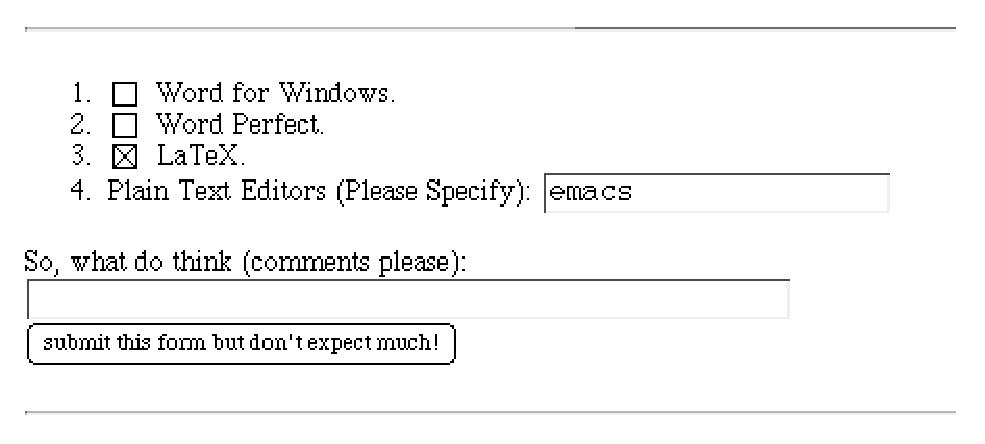
\includegraphics{psfiles/eform}}}
    \end{center}
  \caption{An electronic form.
  In the online version the form would be active.}
  \label{fig_eform}
\end{figure}
\end{latexonly}



\index{rawhtml@\Lc{rawhtml}}%
\paragraph*{\Lc{beginrawhtml}...\Lc{endrawhtml}\label{endrawhtml}}
This is an alternative way to specify a chunk of raw \texttt{HTML} code,
using the old \AmS-style of delimiting environments.
Use of this style is discouraged; 
the \env{rawhtml} \htmlref{environment}{rawhtml} is preferred.%

\index{comment@\env{comment} environment}%
\index{environment!comment@\env{comment}}%
\paragraph*{\Lc{begin\char123comment\char125}\label{comment}}
This environment is simple for the convenience of ``commenting-out''
large sections of source code.
The contents of this environment is completely ignored,
both in the \LaTeX{} and \texttt{HTML} versions.
Such an environment is already used in \AmS-\LaTeX,
and perhaps with other packages.
It is defined here for its general utility.

\noindent
To insert \texttt{SGML}-style comments into the \texttt{HTML} files,
use the \env{rawhtml} environment as follows.
%begin{latexonly}
\begin{small}
%end{latexonly}
\begin{verbatim}
\begin{rawhtml}
<!--  this text is treated as a comment
      perhaps extending over several lines 
-->
\end{rawhtml}
\end{verbatim}
%begin{latexonly}
\end{small}
%end{latexonly}%

\noindent
Note the \hyperref[page]{warning}{warning on page~}{}{env:warn}
concerning how the environment delimiters should be used in the
\LaTeX{} source code.


\index{latexonly@\Lc{latexonly}}%
\paragraph*{\Lc{comment...\char92endcomment}\label{endcomment}}
This is an alternative way to specify a chunk of material intended
to be ignored in both the \LaTeX{} and \texttt{HTML} versions,
using the old \AmS-style of delimiting environments.
Use of this style (though convenient for typing) is discouraged,
since it is not as reliable as using the \env{comment} \htmlref{environment}{comment}.


\subsection{Arbitrary Tags and Attributes\label{sec:arbtags}}%
%\section{Arbitrary Tags and Attributes\label{sec:arbtags}}%
%
For version 97.1 of \latextohtml\ there is a new command which provides 
an extremely flexible way to include \texttt{HTML} 3.2 tags, along with
any values for the ``attributes'' of that tag, if desired.
\begin{quote}
\Lc{HTMLcode}\verb|[|\Meta{attribs}\verb|]{|\Meta{tag}\verb|}|\label{HTMLtag}\\
\Lc{HTMLcode}\verb|[|\Meta{attribs}\verb|]{|\Meta{tag}\verb|}{|\Meta{contents}\verb|}|
\end{quote}
When the \Meta{tag} also needs a closing tag (e.g \texttt{<I>...</I>})
the \Meta{contents} \emph{must} be given, enclosed in braces.
Both the opening and closing tags then will be placed correctly.

\smallskip
\begin{quotation}
\textbf{Warning: } 
In version 97.1 this command was actually called \Lc{HTML}.
However style files may well define \Lc{HTML} to mean something else,
like a styled version of the \texttt{HTML} acronym. 
So in version 98.1 the name has been changed to \Lc{HTMLcode}.

If no other definition of \Lc{HTML} exists, then this command \emph{will}
be defined, to work the same as \Lc{HTMLcode}. 
\end{quotation}

An important aspect of this is that any of the \Meta{tag},
\Meta{attribs} and \Meta{contents} may be given wholly
by expanding a \LaTeX{} macro, or may contain arbitrary macros, 
perhaps including other \Lc{HTMLcode} commands.
\hyperref{The following table}{The contents of Figure~}{}{ex:HTMLcode} 
was constructed using this feature; its \LaTeX{} source follows.

\HTMLcode[50\% 3 noshade center]{HR}

\begin{htmlonly}
\begin{figure}
\begin{makeimage}
\end{makeimage}
\setlength{\captionwidth}{7cm}
\newcommand{\myalign}{center}
\newcommand{\mylist}{UL}
\newcommand{\myitem}[2]{\HTMLcode[disc]{LI}{\simpletest{#1}{#2}}}
\newcommand{\simpletest}[2]{%
 \HTMLcode{#1}{ a simple test of ``#2'',} using \HTMLcode{CODE}{<#1>} .}
\newcommand{\tableopts}{10,border=5}

\newcommand{\tablelist}[4][\myalign]{\HTMLcode[#1]{DIV}{
\HTMLcode[\tableopts]{TABLE}{
\HTMLcode[bottom]{CAPTION}{
#3
}\HTMLcode{TR}{\HTML{TD}{
\HTMLcode{#2}{
#4
}}}
}}\HTMLcode[all]{BR}}

\tablelist[\myalign]{\mylist}{%
\textbf{A listing of the different text styles available in HTML 3.2}}{%
\myitem{B}{bold-face}
\myitem{I}{italics}
\myitem{TT}{teletype-text}
\myitem{U}{underlining}
\HTMLcode[circle]{LI}{\simpletest{STRIKE}{strikeout}}
\myitem{EM}{emphasis style}
\myitem{STRONG}{strong style}
\myitem{CODE}{code style}
\myitem{CITE}{citation style}
\myitem{DFN}{definition style}
\HTMLcode[square]{LI}{\simpletest{SAMP}{sample style}}
\HTMLcode[square]{LI}{\simpletest{KBD}{keyboard style}}
\myitem{VAR}{variable style}}
%
 \caption{Example use of macros for raw \texttt{HTML} code.}
 \label{ex:HTMLcode}
\end{figure}
\end{htmlonly}
%
\begin{latexonly}
\begin{figure}[ht]
\begin{center}
  \fbox{\scalebox{.7}{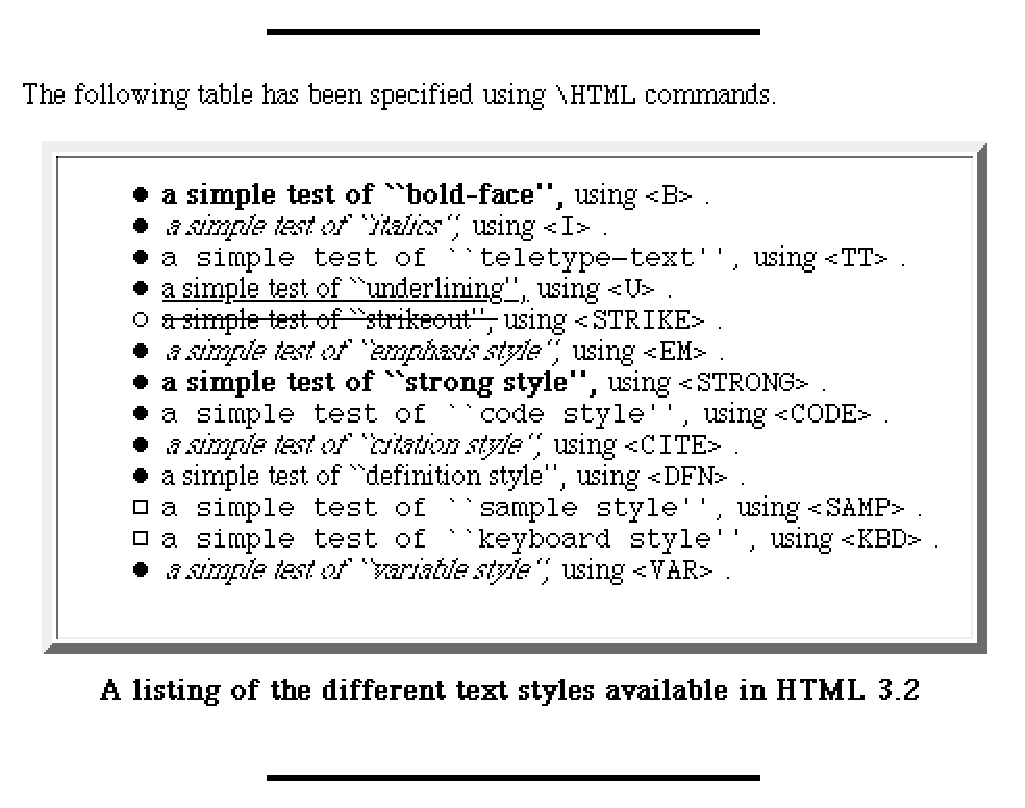
\includegraphics{psfiles/HTMLtab}}}
 \caption{Example use of macros for raw \texttt{HTML} code.}
 \label{ex:HTMLcode}
\end{center}
\end{figure}
\end{latexonly}

\HTMLcode[50\% 3 noshade center]{HR}

%begin{latexonly}
\begin{small}
%end{latexonly}
\begin{verbatim}
\newcommand{\myalign}{center}
\newcommand{\mylist}{UL}
\newcommand{\myitem}[2]{\HTMLcode[disc]{LI}{\simpletest{#1}{#2}}}
\newcommand{\simpletest}[2]{%
 \HTMLcode{#1}{ a simple test of ``#2'',} using \HTMLcode{CODE}{<#1>} .}
\newcommand{\tableopts}{10,border=5}

\newcommand{\tablelist}[4][left]{\HTMLcode[#1]{DIV}{
\HTMLcode[\tableopts]{TABLE}{
\HTMLcode[bottom]{CAPTION}{
#3
}\HTMLcode{TR}{\HTMLcode{TD}{
\HTMLcode{#2}{
#4
}}}
}}\HTMLcode[all]{BR}}

\tablelist[\myalign]{\mylist}{%
\textbf{A listing of the different text styles available in HTML 3.2}}{%
\myitem{B}{bold-face}
\myitem{I}{italics}
\myitem{TT}{teletype-text}
\myitem{U}{underlining}
\HTMLcode[circle]{LI}{\simpletest{STRIKE}{strikeout}}
\myitem{EM}{emphasis style}
\myitem{STRONG}{strong style}
\myitem{CODE}{code style}
\myitem{CITE}{citation style}
\myitem{DFN}{definition style}
\HTMLcode[square]{LI}{\simpletest{SAMP}{sample style}}
\HTMLcode[square]{LI}{\simpletest{KBD}{keyboard style}}
\myitem{VAR}{variable style}}
\end{verbatim}
%begin{latexonly}
\end{small}
%end{latexonly}

\HTMLcode[50\% 3 noshade center]{HR}

\noindent
The above code demonstrates many aspects of the way \Lc{HTML}
commands can be used.
%
\begin{htmllist}\htmlitemmark{GreenBall}
\item [nesting: ] 
\Lc{HTML} commands can be nested to arbitrary depth.
%
\item [macros: ] 
Macros can be used to specify all or part of each argument.
%
\item [within macros: ] 
\Lc{HTMLcode} commands work correctly within the expansions of other macros.
%
\item [attribute values: ]
Information within \Meta{attribs} can be specified in a very
loose way, as a comma-separated list of key/value pairs
or as single values. \\
Not even the commas are necessary: space(s), \Meta{tab}s 
or newlines are equally effective.
Indeed the horizontal rules preceding and following the table were 
specified by:
\begin{quote}
\begin{verbatim}
\HTMLcode[50\% 3 noshade center]{HR}
\end{verbatim}
\end{quote}
%
\item [attribute names: ]
Usually it is \emph{not necessary} to know the names of the
attributes to the tags that are to be used. It is sufficient
just to give the values; these will be matched to the
appropriate attribute, according to the type of data required.
(If names are given, these are case-insensitive.)
%
\item [newlines: ] 
Although \LaTeX{} ignores linebreaks within the source code,
this is not so with \latextohtml. 
The strange spreading-out of the definition of the
\Lc{tablelist} command above was done with the purpose
solely of making the code in the resulting \texttt{HTML} files 
more easily readable, to a human.
(As most browsers ignore those newlines anyway, 
more compact code would have rendered the same on-screen.)
\end{htmllist}

\medskip\noindent
Some further aspects of the use of this \Lc{HTML}
command are not apparent from the above example. 

\begin{htmllist}\htmlitemmark{RedBall}
%
\item [invalid \Meta{tag}\,: ]
If a \Meta{tag} is specified that is not part of the 
\texttt{HTML} 3.2 specifications, then it and its attributes are 
not placed into the \texttt{HTML} document created by \latextohtml.
Any \Meta{contents} \emph{is} included as ordinary data; 
i.e. as text in paragraphs, etc.

\item [required attributes: ] 
Some tags have attributes which are required to have values,
if that tag is to be included in an \texttt{HTML} document.
Using the \Lc{HTML} command, if any such attribute
is not given an appropriate value then the tag is ignored.
Any \Meta{contents} are included in the document, 
as ordinary character data.

\item [valid HTML\,: ] 
Currently there is \emph{no} checking that the \Meta{contents}
of a \Meta{tag} contains only data (perhaps including other tags)
allowed by the DTD for \texttt{HTML} 3.2.
\begin{quote}
\textit{The requirement to produce valid \texttt{\upshape HTML} 
currently rests with the user.}
\end{quote}
This issue will be addressed in forthcoming revisions of \latextohtml.

\item [extra attributes and values: ]
The list of attributes for a \Meta{tag} can include
key-value pairs whose keys do not match any valid
attribute for the \Meta{tag}.
Such key-value pairs are simply ignored.
Similarly extra data values are ignored, 
as are values that do not match the
requirements for any valid attribute.

\item [attributes with similar data-types: ]
Several attributes to a \Meta{tag} may use values having 
the same or similar data-types. First any key-value pairs
are processed. Remaining values are allocated 
to those attributes which do not already have a value.
An ordering of the attributes is used, based on a perceived likelihood 
of each attribute being required to be changed from its default setting.

\end{htmllist}


\subsection{Conditional Text\label{sec:latexonly}}%
%\section{Conditional Text\label{sec:latexonly}}%
\tableofchildlinks*
\index{latexonly@\env{latexonly} environment}%
\index{htmlonly@\env{htmlonly} environment}%
\index{environment!htmlonly@\env{htmlonly}}%
\index{environment!latexonly@\env{latexonly}}%
\index{conditional text!scoped variant}\html{\\}%
\paragraph*{\Lc{begin\char123latexonly\char125} and 
\Lc{begin\char123htmlonly\char125}\label{latexonly}\label{htmlonly}}
Conditional text can be specified
using the environments \env{latexonly} and \env{htmlonly}. 
These allow writing parts of a document which are intended 
only for electronic delivery or only for paper-based delivery.

This would be useful for example in adding a long description of a
multi-media resource in the paper version of a document. 
Such a description would be redundant in the electronic version, 
as the user can have direct access to this resource. 

\medskip\goodbreak\noindent
Here is an example of the use of the \env{latexonly} environment,
used \hyperref[page]{earlier in}{on page~}{ of}{eform} this manual:
%begin{latexonly}
\begin{small}\indent
%end{latexonly}
\Lc{begin}\verb|{latexonly}|
\latex{\vskip-\baselineskip\vskip-\baselineskip}
\begin{verbatim}
\begin{figure}
    \begin{center}
    \fbox{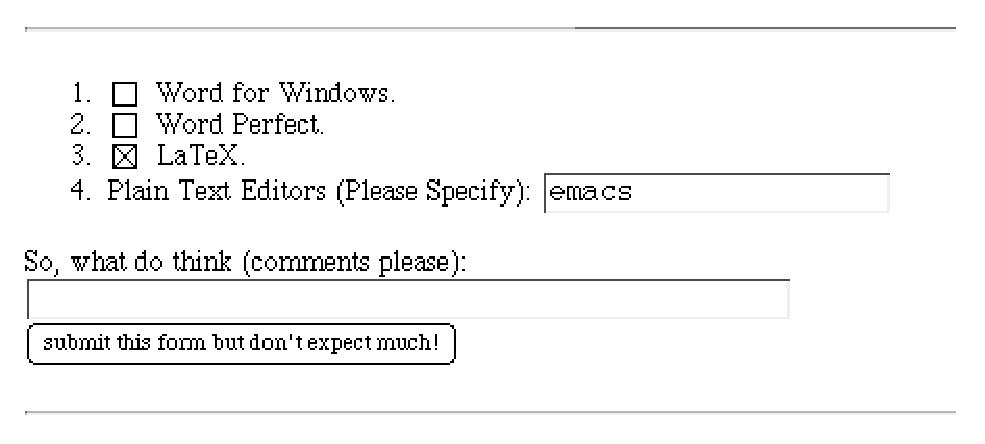
\includegraphics[width=4in]{psfiles/eform}}
    \end{center}
    \caption{An electronic form. Of course in the online version of this
     document the form above would be active.}
\end{figure}
\end{verbatim}
\latex{\nobreak\vskip-\baselineskip\nobreak\indent\indent}%
\Lc{end}\verb|{latexonly}|
%begin{latexonly}
\end{small}\goodbreak\medskip
%end{latexonly}

\noindent
Note the \hyperref[page]{warning}{warning at the bottom of page~}{}{env:warn}
concerning how the environment delimiters should be used in the
\LaTeX{} source code.


\index{htmlonly@\Lc{htmlonly}}%
\paragraph*{\Lc{htmlonly...\char92endhtmlonly}\label{endhtmlonly}}
This is an alternative way to specify a chunk of material intended
for the \texttt{HTML} version only,
using the old \AmS-style of delimiting environments.
Use of this style is discouraged; 
the \env{htmlonly} \htmlref{environment}{htmlonly} is preferred.%


\index{latexonly@\Lc{latexonly}}%
\paragraph*{\Lc{latexonly...\char92endlatexonly}\label{endlatexonly}}
This is an alternative way to specify a chunk of material intended
for the \LaTeX{} typeset version only,
using the old \AmS-style of delimiting environments.
Use of this style is discouraged; 
the \env{latexonly} \htmlref{environment}{latexonly} or the unscoped 
\htmlref{\texttt{\%begin\char123latexonly\char125}}{unlatexonly} 
construction are preferred.%

\smallskip\noindent
Note the \hyperref[page]{warning}{warning at the bottom of page~}{}{env:warn}
concerning how the environment delimiters should be used in the
\LaTeX{} source code.


\index{conditional text!shorthand notation}%
\index{latex@\Lc{latex}}%
\index{html@\Lc{html}}%
\index{latexhtml@\Lc{latexhtml}}\html{\\}%
\paragraph*{\Lc{latex}, \Lc{html} and \Lc{latexhtml}\label{latexhtml}}
There are also shorthand notations to accomplish the same thing 
as in the \env{latexonly} \htmlref{environment}{latexonly} and \env{htmlonly} 
\htmlref{environment}{htmlonly}, but with less typing.
\begin{itemize}
\item 
The \Lc{latex}\verb|{...}| command causes everything within the braces 
to be processed by \LaTeX, but ignored by \latextohtml.
\item  
Conversely, the \Lc{html}\verb|{...}| command causes everything within the braces 
to be ignored by \LaTeX{} and processed by \latextohtml.  
\item  
Finally the command \Lc{latexhtml}\verb|{...}{...}| causes everything 
within the first set of braces to be processed exclusively by \LaTeX, 
with the contents of the second set of braces processed solely by \latextohtml.%
\end{itemize}
\textbf{Warning: }
Only small pieces of text work reliably in this way. 
With whole paragraphs or contained sub-environments,
the ``conditional'' environments should be used instead.

\index{conditional text!without scope}%
\index{beginlatex@\texttt{\%{}begin\char123latexonly\char125}}%
\index{endlatex@\texttt{\%{}end\char123latexonly\char125}}%
\paragraph*{\texttt{\%begin\char123latexonly\char125}\label{unlatexonly}}
Another variant of the \env{latexonly} environment is available, 
in which everything between 
\texttt{\%begin\{latexonly\}} and \texttt{\%end\{latexonly\}}
is ignored by \latextohtml.  
The difference is that the \env{latexonly} environment 
puts the contents into a group, in which all definitions are local.
There is no such scoping with the \texttt{\%begin...\%end} variant,
since \LaTeX{} sees the initial \texttt{\%}s simply as starting comments.%

\medskip
\index{conditional text!example}\html{\\}\noindent
The following example should clarify what happens:
%begin{latexonly}
\begin{small}
%end{latexonly}
\begin{verbatim}
\newcommand{\A}{The letter A.}
\newcommand{\B}{The letter B.}
\end{verbatim}
\indent\indent\indent\texttt{\char92begin\{latexonly\}}\\
\indent\indent\verb|\renewcommand{\A}{Not the letter A.}|\\
\indent\indent\texttt{\char92end\{latexonly\}}\\
\indent\indent\texttt{\%begin\{latexonly\}}\\
\indent\indent\verb|\renewcommand{\B}{Not the letter B.}|\\
\indent\indent\texttt{\%end\{latexonly\}}
\begin{verbatim}
\begin{document}
\A \B
\end{document}
\end{verbatim}
%begin{latexonly}
\end{small}
%end{latexonly}
If you process this with \LaTeX, the result is: 
\quad\quad The letter A. Not the letter B.

\smallskip\noindent
Note the \hyperref[page]{warning}{warning at the bottom of page~}{}{env:warn}
concerning how the environment delimiters should be used in the
\LaTeX{} source code.

\medskip\index{conditional text!avoid using counters}\html{\\}\noindent
\textbf{Warning: }% 
Be careful when using \LaTeX{}  commands which alter the values of counters 
(e.g.\ numbered figures or equations) in conditional text, because this may 
cause the counter values in the electronic version to lose synchronisation 
with the values of the corresponding counters in the \LaTeX{} version.


\htmlrule[width=300]
\index{imagesonly@\env{imagesonly} environment}%
\index{environment!imagesonly@\env{imagesonly}}%
\paragraph*{\Lc{begin\char123imagesonly\char125}\label{imagesonly}}
This environment is used to put \LaTeX{} code into the \fn{images.tex} file,
to be used when generating images. Typically this is used to add commands to
the preamble of \fn{images.tex}, such as setting the text or background color.
However code can be added at any other point as well; 
e.g.\ to change the background color of all images after a certain point in the document. 

\smallskip\noindent
Note the \hyperref[page]{warning}{warning at the bottom of page~}{}{env:warn}
concerning how the environment delimiters should be used in the
\LaTeX{} source code.


\index{makeimage@\env{makeimage} environment}%
\index{environment!makeimage@\env{makeimage}}%
\paragraph*{\Lc{begin\char123makeimage\char125}\label{makeimage}}
This is a special environment which forces an image to be made of its contents.
That is, one gets effectively a snapshot of a portion of a page
that has been typeset using \LaTeX. 
Within the normal \LaTeX{} typeset version of the document, this environment 
is completely transparent, adding its contents to the page as usual.

\index{makeimage@\env{makeimage} environment!inside@inside a \env{figure}}\html{\\}%
One further important use of the \env{makeimage} environment is as follows.
If a \env{makeimage} environment occurs as a sub-environment within 
a \env{figure} environment, then an image will \emph{not} be made of the
\env{figure}'s contents. Instead, the contents are treated as normal text,
each part being handled as if there were no \env{figure} at all,
except that everything is placed within a single cell of a
\HTMLtag{TABLE}...\HTMLtag{/TABLE} construction in \HTMLiii. 
The contents of any \Lc{caption}
commands are placed between \HTMLtag{CAPTION}...\HTMLtag{/CAPTION} tags 
for the \HTMLtag{TABLE}.

\index{makeimage@\env{makeimage} environment!empty sub-environment}\html{\\}%
Normally an image of the entire contents of the \env{figure} would be
placed within the single cell of the \HTMLtag{TABLE}.
Now images are made of any subparts of those \env{figure}'s contents 
that really need it, in particular the \env{makeimage} sub-environments.
An empty \env{makeimage} sub-environment does not generate an image of itself,
yet still it inhibits an image being made of the whole \env{figure}.
These comments apply also to \env{table} environments.



\subsection{Symbolic References shown as Hyperized Text\label{hyperized}%
%\section{Symbolic References shown as Hyperized Text\label{hyperized}%
\index{references@references\protect\label{IIIrefs}}}%
\tableofchildlinks*
\index{cross-references!|see{\htmlref{references}{IIIrefs}}}%
\index{references!symbolic\label{IIIsymref}}\index{symbolic labels|(}%
\index{references!numeric}%
\index{references!iconic}\html{\\}\noindent
In printed documents cross-references are shown 
through a \emph{numeric or symbolic indirection} 
e.g.\ ``see Figure 1'' (numeric indirection), 
or ``see section `Changes'~'' (symbolic indirection).  
\latextohtml{} can mirror this mechanism using the same numeric 
or symbolic references,
or when these are not appropriate by using iconic references.

\index{references!without indirection}%
\index{references!highlighted text}\html{\\}%
In a hypertext document however, cross-references can be shown 
without any indirection, just by highlighting a relevant piece of text. 
This can make a document more readable as it removes unnecessary
information. 

\index{hyperref@\Lc{hyperref}}%
\paragraph*{\Lc{hyperref}\label{hyperref}}
A single new \LaTeX{} command \Lc{hyperref} can be used for
specifying how a cross-reference should appear, 
both in the printed document and in the hypertext version.
For example, assuming that the label \verb|{sec:cond}|\label{sec:cond} 
is defined somewhere within a document, 
the command \Lc{hyperref}, taking 4 arguments,
can be used in that document as follows:
\index{hyperref@\Lc{hyperref}}%
\index{conditional text}%
%begin{latexonly}
\begin{small}
%end{latexonly}
\begin{verbatim}
\emph{Is the concept of
\hyperref
               % This will be highlighted in the hypertext version
{conditional text}                      % argument #1
               % This will be shown in the printed version 
               % followed by a numeric reference ...      
{conditional text (see Section }        % argument #2
               % ... followed by this text
{ for more information)}                % argument #3
               % This is the common label 
{sec:cond}                              % argument #4
a good idea? }
\end{verbatim}
%begin{latexonly}
\end{small}
%end{latexonly}

\noindent
Here is how it will be shown:
\begin{quote}
\emph{Is the concept of
\hyperref
% This will be highlighted in the hypertext version
{conditional text}
% This will be shown in the printed version  
% followed by a numeric reference ...      
{conditional text (see Section }  
% ... followed by this text
{ for more information)} 
% This the common label 
{sec:cond}
a good idea? }
\end{quote}

\begin{htmlonly}
In the printed version what would appear is:
\begin{quote}
\emph{Is the concept of conditional text (see Section 4.2 for more information) 
a good idea?}
\end{quote}
\end{htmlonly}

\begin{latexonly}%
In the hypertext version what would appear is:
\begin{quote}
\emph{Is the concept of \underline{conditional text} a good idea?}
\end{quote}
(Of course \underline{conditional text} would be an active hypertext link.)
\end{latexonly}

\bigskip\htmlrule[50\% center]
\noindent
An extended syntax for \Lc{hyperref} uses an optional argument, 
which determines what information is to be placed in the \LaTeX{} version
of the document. The value of this optional argument can also affect 
the number of required arguments. 
These forms are recognised:

%begin{latexonly}
\begin{small}
%end{latexonly}
\begin{quote}\label{hypernoref}
\Lc{hyperref}\verb|[ref]{|\Meta{HTML-text}\verb|}{|\Meta{LaTeX-text}\verb|}{|\Meta{post-LaTeX}\verb|}{|\Meta{label}\verb|}|\\
\Lc{hyperref}\verb|{|\Meta{HTML-text}\verb|}{|\Meta{LaTeX-text}\verb|}{|\Meta{post-LaTeX}\verb|}{|\Meta{label}\verb|}|\medskip

\Lc{hyperref}\verb|[pageref]{|\Meta{HTML-text}\verb|}{|\Meta{LaTeX-text}\verb|}{|\Meta{post-LaTeX}\verb|}{|\Meta{label}\verb|}|\\
\Lc{hyperref}\verb|[page]{|\Meta{HTML-text}\verb|}{|\Meta{LaTeX-text}\verb|}{|\Meta{post-LaTeX}\verb|}{|\Meta{label}\verb|}|\medskip

\Lc{hyperref}\verb|[noref]{|\Meta{HTML-text}\verb|}{|\Meta{LaTeX-text}\verb|}{|\Meta{label}\verb|}|\\
\Lc{hyperref}\verb|[no]{|\Meta{HTML-text}\verb|}{|\Meta{LaTeX-text}\verb|}{|\Meta{label}\verb|}|
\end{quote}
%begin{latexonly}
\end{small}
%end{latexonly}

\noindent
The first two are the defaults, where \LaTeX{} 
uses \Lc{ref}\verb|{|\Meta{label}\verb|}|.
With the next two \LaTeX{} uses \Lc{pageref}\verb|{|\Meta{label}\verb|}|,
while with the final two \LaTeX{} completely ignores the \Meta{label},
setting just the \Meta{LaTeX-text}.

\medskip
\index{hyperref@\Lc{hyperref}!pageref@\Lc{pageref} example}%
\html{\\}\noindent
For creating hyperlinks to other documents
using symbolic reference \Meta{label}s, 
see also the \Lc{externalref} 
\hyperref[page]{command}{command, described on page~}{}{externref}.

\medskip\noindent
The preceding paragraph is an example of the use of the \Lc{hyperref[page]} option.
Its source code is:
%begin{latexonly}
\begin{small}
%end{latexonly}
\begin{verbatim}
For creating hyperlinks to other documents
using symbolic reference \Meta{label}s, 
see also the \Lc{externalref} 
\hyperref[page]{command}{command, described on page~}{}{externref}.
\end{verbatim}
%begin{latexonly}
\end{small}
%end{latexonly}
\begin{htmlonly}
which appears in the \LaTeX{} typeset version as:
\begin{quote}
For creating hyperlinks to other documents
using symbolic reference \Meta{label}s, see also the
\Lc{externalref} command, described on page~31.
\end{quote}
\end{htmlonly}
\begin{latexonly}
which appears in the \texttt{HTML} version as:
\begin{quote}
For creating hyperlinks to other documents, using symbolic reference \Meta{label}s, 
see also the \Lc{externalref} \underline{command}.
\end{quote}
with the \underline{command} being an active hyperlink.
\end{latexonly}
\smallskip\noindent
In fact both \Lc{hyperref} and the \Lc{htmlref} command, to be described next,
permit textual hyperlinks based on symbolic \Meta{label}s from external files.


\index{htmlref@\Lc{htmlref}}%
\index{html.sty@\texttt{html.sty} style-file}
\paragraph*{\Lc{htmlref}\label{htmlref}}
Another command also defined in \fn{html.sty} is \Lc{htmlref} 
which has the same effect as \Lc{hyperref}
during the conversion to \texttt{HTML}.
It takes two arguments, some text and a label. 
In the \texttt{HTML} version the
text will be ``hyperized'', pointing to the label. 
In the paper version the text will be shown as it is 
and the label will be ignored; e.g.
%
\index{htmlref@\Lc{htmlref}!easy to make links}%
%begin{latexonly}
\begin{small}
%end{latexonly}
\begin{verbatim}
With \verb|\htmlref| \htmlref{it's easy to make links}{fig:example}.
\end{verbatim}
%begin{latexonly}
\end{small}
%end{latexonly}
which produces:
\begin{quote}
With \Lc{htmlref} \htmlref{it's easy to make links}{fig:example}.
\end{quote}
\begin{htmlonly}
In the \LaTeX{} typeset version it will appear simply as:
\begin{quote}
With \Lc{htmlref} it's easy to make links.
\end{quote}
\end{htmlonly}
\begin{latexonly}
In the \texttt{HTML} version it is shown as:
\begin{quote}
With \Lc{htmlref} \underline{it's easy to make links}.
\end{quote}
\end{latexonly}
\html{\\}
\goodbreak

\subsection{Hypertext Links in Bibliographic References (Citations)}%
%\section{Hypertext Links in Bibliographic References (Citations)}%
\tableofchildlinks*
\index{references!bibliographic}\index{bibliography|(}%
\index{bibliography!bibliographic database}%
\index{bibliography!using .bib@using \texttt{.bib} file}\html{\\}%
If a report or a book that is cited (using the \Lc{cite} command) 
is available (or there is information about it) on the World-Wide
Web, then it is possible to add the appropriate hypertext links
in your bibliographic database (the \texttt{.bib}) file. 

\bigskip
\index{bibliography!example using URLs}%
\index{bibliography!string commands@\texttt{\char64 string} commands}%
\index{LaTeX blue book@\LaTeX{} blue book}\html{\\}%
\noindent
Here is an example of a bibliographic entry for the original
\LaTeX{} \cite{lamp:latex} blue book:\nobreak
%begin{latexonly}
\begin{small}
%end{latexonly}
\begin{verbatim}
@string{tugURL="\htmladdnormallink
{http://www.tug.org/}{http://www.tug.org}"}

@string{danteURL="\htmladdnormallink
{http://www.dante.de/}{http://www.dante.de}"}

@book{lamp:latex,
title = "LaTeX User's Guide \& Reference Manual, 2nd edition",
year = 1994 ,
author = "Leslie Lamport",
Publisher = "Addison--Wesley Publishing Company, Inc.",
note = "Online information on {\TeX} and {\LaTeX} is available at "
 # tugURL # " and " # danteURL }
\end{verbatim}
%begin{latexonly}
\end{small}
%end{latexonly}
See the \htmlref{bibliography}{biblio} for how this will appear.\html{\\}
No other modifications are required; \LaTeX{} and Bib\TeX{} should work as normal.
%
\index{bibliography!string commands@\texttt{\char64string} commands}%
Note that it would be sensible to put the \texttt{@string} commands
into a separate file, \fn{urls.bib} say, 
loaded with the main file via\html{\\} \verb|\bibliography{urls,...}|.%

\index{citations!natbib@\env{natbib} package}%
\index{bibliography!natbib@\env{natbib} package}%
\index{citations!Harvard style!handled@handled by \env{natbib}}%
The \env{natbib} package, written for \LaTeX{} by \PatrickDaly,
provides even more flexibility in the way a reference may be cited. 
All the features of \htmlref{this package}{natbib} are implemented 
for \latextohtml{} via the \fn{natbib.perl} file.
(Indeed there is even a mode whereby \env{natbib} handles
the Harvard style of citation. 
This requires loading also the \env{nharvard} \htmlref{package}{nharvard}.)

\medskip
\noindent\textbf{Thanks...} to \Wilck\ for the bulk of the work 
in producing this extension, and to \RossMoore\ for 
necessary adjustments to allow it to work correctly with the 
\htmlref{document segmentation strategy}{Segmentation}.


\index{hypercite@\Lc{hypercite}}%
\paragraph*{\Lc{hypercite}\label{hypercite}}
Analogous to \Lc{hyperref} is the \Lc{hypercite} command,
which allows a free-form textual hyperlink to the bibliography,
whereas the \LaTeX{} typeset version contains the usual citation code.
The allowed syntax is as follows.
%begin{latexonly}
\begin{small}
%end{latexonly}
\begin{quote}
\Lc{hypercite}\verb|[int]{|\Meta{HTML-text}\verb|}{|\Meta{LaTeX-text}%
\verb|}{|\Meta{opt-LaTeX}\verb|}{|\Meta{label}\verb|}|\\
\Lc{hypercite}\verb|[cite]{|\Meta{HTML-text}\verb|}{|\Meta{LaTeX-text}%
\verb|}{|\Meta{opt-LaTeX}\verb|}{|\Meta{label}\verb|}|\\
\Lc{hypercite}\verb|{|\Meta{HTML-text}\verb|}{|\Meta{LaTeX-text}%
\verb|}{|\Meta{opt-LaTeX}\verb|}{|\Meta{label}\verb|}|\medskip

\Lc{hypercite}\verb|[nocite]{|\Meta{HTML-text}\verb|}{|\Meta{LaTeX-text}%
\verb|}{|\Meta{label}\verb|}|\\
\Lc{hypercite}\verb|[no]{|\Meta{HTML-text}\verb|}{|\Meta{LaTeX-text}%
\verb|}{|\Meta{label}\verb|}|\\
\Lc{hypercite}\verb|[ext]{|\Meta{HTML-text}\verb|}{|\Meta{LaTeX-text}%
\verb|}{|\Meta{label}\verb|}|
\end{quote}
%begin{latexonly}
\end{small}
%end{latexonly}
The first three forms are equivalent; 
\LaTeX{} uses \Lc{cite}\verb|[|\Meta{opt-LaTeX}\verb|]|\Meta{label}\,,
after placing the \Meta{LaTeX-text}.
Note that \verb|{|\Meta{opt-LaTeX}\verb|}| \emph{must} be specified, 
even if empty `\verb|{}|'.

Similarly the latter three forms are equivalent, 
with \LaTeX{} using \Lc{nocite}\verb|{|\Meta{label}\verb|}|\,, 
to force the particular reference to appear on the bibliography page, 
even though no explicit marker is placed at this point.
(Thus there is no need for an optional  \Meta{opt-LaTeX} argument.)\html{\\}
Within the \texttt{HTML} version a hyperlink is produced when the \Meta{HTML-text} 
is not empty. External label files are also searched, 
in order to match the symbolic \Meta{label}, see also 
\hyperref[page]{\Lc{externalcite}}{\Lc{externalcite} on page~}{}{externcite}.

\smallskip\noindent\label{hyperciteXmpl}%
\index{hypercite@\Lc{hypercite}!example}%
\index{htmlcite@\Lc{htmlcite}!example}\html{\\}\noindent
\htmlref{Earlier}{hypcites} in this manual the following source code was used:
%begin{latexonly}
\begin{small}
%end{latexonly}
\begin{verbatim}
commands described in the \LaTeX{} \htmlcite{blue book}{lamp:latex}, 
...
as well as many other \LaTeX{} constructions, such as are described in 
the \LaTeX{} \hypercite{\emph{Companion}}{\emph{Companion}}{}{goossens:latex} 
and \LaTeX{} \hypercite{\emph{Graphics Companion} (e.g.\ \Xy-pic)}%
{\emph{Graphics Companion}}{\Xy-pic}{goossens:latexGraphics};
\end{verbatim}
%begin{latexonly}
\end{small}
%end{latexonly}
which produces:
\begin{quote}
commands described in the \LaTeX{} \htmlcite{blue book}{lamp:latex}, 
\\~~...\\
as well as many other \LaTeX{} constructions, such as are described in 
the \LaTeX{} \hypercite{\emph{Companion}}{\emph{Companion}}{}{goossens:latex} 
and \LaTeX{} \hypercite{\emph{Graphics Companion} (e.g.\ \Xy-pic)}%
{\emph{Graphics Companion}}{\Xy-pic}{goossens:latexGraphics};
\end{quote}
\begin{latexonly}
whereas in the \texttt{HTML} version one sees:
\begin{quote}
commands described in the \LaTeX{} \underline{blue book}, 
\\~~...\\
as well as many other \LaTeX{} constructions, 
such as are described in the \LaTeX{} \underline{\emph{Companion}} 
and  \LaTeX{} \underline{\emph{Graphics Companion} (e.g.\ \Xy-pic)};
\end{quote}
\end{latexonly}
%
\begin{htmlonly}
whereas in the \LaTeX{} typeset version one sees:
\begin{quote}
commands described in the \LaTeX{} blue book,\\
~~...\\
as well as many other \LaTeX{} constructions, such as are described in the \LaTeX{} 
\textit{Companion}[2] and \LaTeX{} \textit{Graphics Companion}[3, \Xy-pic];
\end{quote}
\end{htmlonly}


\index{htmlcite@\Lc{htmlcite}}%
\paragraph*{\Lc{htmlcite}\label{htmlcite}}
Analogous to \Lc{htmlref} is the \Lc{htmlcite} command,
which creates a textual hyperlink to a place on the document's bibliography page, 
but without displaying any reference marker in the \LaTeX{} typeset version.
(See \htmlref{above}{hyperciteXmpl} for an example.)%

The \Lc{externalcite} 
\hyperref[page]{command}{command, described on page~}{, }{externcite}
provides a similar facility when the bibliography page is ``external'';
that is, not part of the current document.%

\index{bibliography|)}



\subsection{Symbolic References between Living Documents\label{external_cross}}%
%\section{Symbolic References between Living Documents\label{external_cross}}%
\tableofchildlinks*
\index{external references|(}
\index{references!to external documents}%
\index{references!symbolic}%
\index{symbolic labels!see also@\emph{see also} 
 \htmlref{references, symbolic}{IIIsymref}}%
\index{labels!symbolic}%
%
The method of the previous section to generated
symbolic \htmlref{hyperized}{hyperized} links can
easily be extended to \emph{external} documents processed by \latextohtml.  
When \latextohtml{} processes a document, it generates a \Perl{} file 
named \Meta{prefix}\fn{labels.pl}
which contains a list of all the symbolic labels that were defined, 
along with their locations.  
The \htmlref{\Meta{prefix}}{prefix} is empty unless otherwise specified, 
to allow different document segments to share the same directory.  

\index{externallabels@\Lc{externallabels}}%
\index{externalref@\Lc{externalref}}%
\paragraph*{\Lc{externallabels}\label{externlabels}}
Links to an external document are then possible once a connection 
is established to that document's \fn{labels.pl} file.  
This connection is established by the \Lc{externallabels} command:%
%
\begin{quote}
%begin{latexonly}
\begin{small}
%end{latexonly}
\Lc{externallabels}\verb|{|\Meta{URL to directory of external document}\verb|}|\\
\verb|               {|\Meta{local copy of external document labels.pl file}\verb|}|
%begin{latexonly}
\end{small}
%end{latexonly}
\end{quote}
%
\index{labels!external}\html{\\}%
The first argument to \Lc{externallabels} should be a URL to 
the directory containing the external document.  
The second argument
should be the full path-name to the \fn{labels.pl} file belonging
to the external document.  Note that for \emph{remote} external documents
it is necessary to copy the \fn{labels.pl} file locally so that it
can be read when processing a local document that uses it.
The command \Lc{externallabels} can be used once for each external
document in order to import the \textit{external labels}\label{externallabels}
into the current document.
A warning is given if \fn{labels.pl} cannot be found.

If a symbolic reference made in either of the commands described
\hyperref{on the previous page}{in Section~}{}{hyperized} is not 
defined within the document itself,
\latextohtml{} will look for that reference in one of the external
files\footnote{Care must be taken to ensure that critical symbolic
references are unique across related documents.}.
After any modifications in an external document 
(sections added/deleted, segmentation into different physical parts, etc.) 
a new \fn{labels.pl} will be generated.  
If the \Lc{externallabels} command in another 
document contains the correct address to an updated copy of
the \fn{labels.pl} file, then the cross-references will be re-aligned
after running the local document through the translator.

\index{labels!internal}\label{internallabels}\html{\\}%
There is also a mechanism analogous to the
\textit{label--ref} pairs of \LaTeX, which can be used only 
within a single document. 
These labels are called \textit{internal labels},
as opposed to the \htmlref{external labels}{externallabels} defined above.
They are used extensively with the document segmentation strategy
described \hyperref{later}{in Section~}{}{Segmentation}.

Either type of label is defined with a \LaTeX{} \Lc{label} command.  
Labels can be referenced \textit{within} a document using a \Lc{ref} command.
When processed by \LaTeX, each \Lc{ref} command is replaced by the 
section number in which the corresponding \Lc{label} occurred.
When processed by the translator, each \Lc{ref} is replaced by 
a hypertext link to the place where the corresponding \Lc{label} occurred.%
 

\index{references!to external documents}%
\index{externalref@\Lc{externalref}}%
\paragraph*{\Lc{externalref}\label{externref}}
This mechanism can be extended to external documents:
\begin{quote}
%begin{latexonly}
\begin{small}
%end{latexonly}
\Lc{externalref}\verb|{|\Meta{symbolic label in remote document}\verb|}|
%begin{latexonly}
\end{small}
%end{latexonly}
\end{quote}
The argument to \Lc{externalref} may be any symbolic label defined 
in the \fn{labels.pl} file of any of the external documents.
Such references to external symbolic labels are then translated
into hyper-links pointing to the external document.%


\index{citations!within external bibliographies}%
\index{externalcite@\Lc{externalcite}}%
\paragraph*{\Lc{externalcite}\label{externcite}}
%
Analogous to \htmlref{\Lc{externalref}}{externref},
the \Lc{externalcite} command is used to create a citation link,
where the bibliography page is not part of the current document.
As with \Lc{externalref} symbolic labels for the bibliography page
must have been loaded using 
\htmlref{\Lc{externallabels}}{externlabels}.

A particularly important use for this is in allowing multiple documents 
to access information in a common bibliographic listing.
For example: all of an author's publications; 
a comprehensive listing of publications in a particular field; 
the (perhaps yearly) output of publications 
from a particular organisation or institution.

\medskip\noindent
\textbf{Thanks...} to \Engberg\ for suggesting this feature.

\index{external references|)}


\subsubsection{Cross-Referencing Example\label{crossrefs}}% 
%\subsection{Cross-Referencing Example\label{crossrefs}}% 
To understand this mechanism better consider 
how you would maintain a link to this section  
(of the hypertext version of this document) from one of your documents,
without using labels.
Sure enough you can get the name of the physical file that this section is in. 
This however is quite likely to change, and any links to it would become invalid. 
\index{link validation!done by hand}%
To update your link, the name of the new file must be found 
and your link changed by hand. 
Also there is no general updating mechanism, so the only way to find
out if your document is pointing to the right place is by actually
following the link, then doing a manual update\footnote{%
Link validation can be done automatically but the updating must be done
manually when filenames have changed (assuming no other symbolic label
mechanism is available).}.

\index{link validation!symbolic labels}\html{\\}%
Next consider how it could be done with symbolic labels. 
First you have to import the labels used in this document 
by copying the file \fn{labels.pl},
saving it in \path{/tmp/labels.pl} say,
then adding anywhere in your document:
%begin{latexonly}
\begin{small}
%end{latexonly}
\begin{verbatim}
\externallabels{http://cbl.leeds.ac.uk/nikos/tex2html/doc/manual}%
               {/tmp/labels.pl}
\end{verbatim}
%begin{latexonly}
\end{small}
%end{latexonly}
After that you can use the label `\texttt{crossrefs}' defined at the beginning of this 
section\footnote{You either have to guess the role of each label by
looking at the \fn{labels.pl} file or by asking the author!} as follows:
%begin{latexonly}
\begin{small}
%end{latexonly}
\begin{verbatim}
\externalref{crossrefs}
\end{verbatim}
%begin{latexonly}
\end{small}
%end{latexonly}
This will be translated into the appropriate hyper-link to this page.
If there are any changes in this document and you would like to
bring your document up-to date, you have to copy 
\fn{labels.pl} again
and rerun the translator on your document. Of course if I move the 
directory containing the \texttt{HTML} files for this document somewhere else, 
then you would have to make a change in the argument of the 
\Lc{externallabels} command to reflect this. 

\index{references!collaboration required}%
It is obvious that some level of collaboration is required between
authors trying to maintain cross-references between different documents. 
Using symbolic labels makes this a lot easier 
(especially for documents written by the same author).
\index{symbolic labels|)}



\subsection{Miscellaneous commands for \texttt{HTML} effects\label{misceffects}}%
%\section{Miscellaneous commands for \texttt{HTML} effects\label{misceffects}}%
\tableofchildlinks*
\index{html.sty@\texttt{html.sty} style-file}%

\noindent
The \env{html} package, through the \LaTeX{} input file \fn{html.sty},
and its \Perl{} counterpart \fn{html.perl}, implements several 
new commands that are intended entirely for effects within the
produced \texttt{HTML} files. In \LaTeX{} these commands, their arguments,
and any optional arguments are completely ignored.

\index{htmlrule@\Lc{htmlrule}}%
\index{visual separation!using \Lc{htmlrule}}%
\paragraph*{\Lc{htmlrule } and 
 \Lc{htmlrule*}\label{htmlrule}}
One such device provided by \fn{html.sty},
is the \Lc{htmlrule} command. 
This puts a horizontal rule into the \texttt{HTML} file only;
being ignored in the \texttt{.dvi} version. 
It is useful to provide extra visual separation between paragraphs,
without creating a new \texttt{HTML} page, 
such as might warrant extra vertical space within the printed version.

\index{htmlrule!htmlrulestar@\Lc{htmlrule*}}%
\index{htmlrule!variants}%
\index{htmlrule!attributes@attributes to the \HTMLtag{HR} tag}%
Much variation can be obtained in the horizontal rule that is produced,
using extended forms of the \Lc{htmlrule} command:
\begin{quote}
%begin{latexonly}
\begin{small}
%end{latexonly}
\Lc{htmlrule}\\
\Lc{htmlrule*}\\
\Lc{htmlrule[}\Meta{attribs}\texttt{]}\\
\Lc{htmlrule*[}\Meta{attribs}\texttt{]}
%begin{latexonly}
\end{small}
%end{latexonly}
\end{quote}
Whereas a ``break'' tag \HTMLtag{BR} normally precedes the \HTMLtag{HR} generated
by the \Lc{htmlrule} command, 
this break is omitted when using the \Lc{htmlrule*} variant. 

\htmlrule[center,width=200]

\noindent
Furthermore, the optional argument \Meta{attribs} can be used to specify 
attributes for \emph{both} the \HTMLtag{HR} and \HTMLtag{BR} tags. 
More specifically, \Meta{attribs} should be a list of attribute-names 
and/or key-value pairs \texttt{\Meta{key}=\Meta{value}} separated by spaces or commas. 
This list is parsed to extract those attributes applicable to the \HTMLtag{HR} tag,
and those applicable to the \HTMLtag{BR} (with the unstarred variant).

\medskip\htmlrule[right,width=200,size=5]
\noindent
Using \HTMLiii, this allows variations to be specified for:
\begin{itemize}
\item 
the (vertical) thickness of the horizontal line in pixels: \texttt{SIZE=\Meta{num}};
\item 
the (horizontal) width of the line in pixels or points: \texttt{WIDTH=\Meta{width}};
\item 
alignment: \texttt{WIDTH=\char34...\char34 } 
taking \texttt{left}, \texttt{right} or \texttt{center};
\item 
removal of the shadowed effect \texttt{NOSHADE};
\item 
positioning of the rule with respect to text-flows: 
\texttt{CLEAR=\char34...\char34 } 
taking \texttt{left}, \texttt{all}, \texttt{right} or \texttt{none}. 
\htmlrule[right,width=200,size=5]
\end{itemize}%
Some examples of these effects appear on 
\latex{the \texttt{HTML} version of} this page.%


\index{strikeout@\Lc{strikeout}}%
\paragraph*{\Lc{strikeout\char123}\Meta{text}\texttt{\char125}\label{strikeout}}
With this command the \Meta{text} is processed as normal in the \texttt{HTML} version,
then placed between \HTMLtag{STRIKE}...\HTMLtag{/STRIKE} tags.
Thus a horizontal line should be drawn through the middle of the \Meta{text}.\html{\\}
Currently the command and the \Meta{text} are ignored in the \LaTeX{} version.%


\index{tableofchildlinks@\Lc{tableofchildlinks}}%
\paragraph*{\Lc{tableofchildlinks }\label{tochlinks}}
As an extra aid to navigation within a long page, 
containing several (sub)subsections or deeper levels of sectioning,
there is the \Lc{tableofchildlinks} command.
This does not generate anything new, for a table of the child links
on or from a page is generated automatically by \latextohtml.

However if this command, or its variant \Lc{tableofchildlinks*},
occurs within the source code to appear on a particular \texttt{HTML} page,
then the child-links table will be placed at that point
where the command occurs. 
Normally a break tag \HTMLtag{BR} is inserted to separate the table of child-links 
from the surrounding text. The \Lc{tableofchildlinks*} omits this extra break
when it would result in too much space above the table.

For example throughout this section of the \latex{\texttt{HTML} version of the }manual, 
all subsections in which several explicit commands have been discussed
have their child-links table placed at the top of the page,
using \Lc{tableofchildlinks*}. 
This helps to quickly find the description of how the commands are used.%


\index{htmlinfo@\Lc{htmlinfo}}%
\paragraph*{\Lc{htmlinfo }\label{htmlinfo}}
Normally an ``About this document...'' page is created at the end
of the \texttt{HTML} document, containing technical information
about how the document was created, by whom, or any other information
contained in the \fn{\$INFO} \htmlref{variable}{infostring}.
This information can be made to appear at any other place within the document 
by specifying \Lc{htmlinfo} at the desired place in the source.
For example, the information may be best suited for the title-page.

The variant \Lc{htmlinfo*} places the information, but leaves out the 
standard ``About this document...'' header. 
Instead the \htmlref{\Lc{htmlhead}}{htmlhead} command 
can be used to place an alternative heading, prior to the \Lc{htmlinfo*} command.
Neither this heading nor the \fn{\$INFO} \htmlref{contents}{infostring} appears 
in the \LaTeX{} typeset version.%


\index{bodytext@\Lc{bodytext}}%
\paragraph*{\Lc{bodytext\char123}\Meta{options}\texttt{\char125}\label{bodytext}}
The text and background colors, and colors for the text of hypertext links can
be set on an \texttt{HTML} page by giving appropriate attributes 
with the \HTMLtag{BODY ...} tag. This is particularly easy to do
using the \Lc{bodytext} command, 
which simply inserts the \Meta{code} as the desired list of attributes.%

\medskip
\index{bodytext@\Lc{bodytext}!no checking for valid attributes}\html{\\}%
\noindent
\textbf{Warning: }Any previous settings for the \HTMLtag{BODY ...} tag
are discarded. Furthermore no checking is done to verify whether the given \Meta{options}
indeed contains a list of attributes and values valid for the \HTMLtag{BODY ...} tag.\html{\\}
When using \Lc{bodytext} you are assumed to know precisely what you are doing!

\medskip\noindent
Other packages contain commands which alter the contents of the \HTMLtag{BODY ...} tag;
notably the \fn{color.perl} implementation of \LaTeX's \env{color} package,
and the (prototype) \env{frames} package, by \Wilck\ and \RossMoore.
In both these packages the requested information is checked for
validity as an attribute within the \HTMLtag{BODY ...} tag.

\index{htmlbody@\Lc{htmlbody}}%
\paragraph*{\Lc{htmlbody\char123}\Meta{options}\texttt{\char125}\label{htmlbody}}
This is similar to the \Lc{bodytext} command, except that it adds the
value of an attribute, or allows an existing value to be changed.
Thus it can be used to alter just a single one of the text and background colors, 
colors for the text of hypertext links or add a background pattern.
The \Meta{options} are given as key-value pairs; some checking is done to ensure 
the validity of the attributes whose values are being set.%

\index{htmlbase@\Lc{htmlbase}}%
\paragraph*{\Lc{htmlbase\char123}\Meta{URL}\texttt{\char125}\label{htmlbase}}
This specifies that the given \Meta{URL} be included in the \HTMLtag{HEAD} section
of each \texttt{HTML} page via a tag: 
\texttt{<BASE HREF=\char34\Meta{URL}\char34}.\html{\\}
Such a feature is particularly useful\dots 
\begin{itemize}
\item
when preparing a document whose final location may be different from where it was created; 
By making all internal references be relative (to the the provided \Meta{URL}),
a whole directory tree containing the document 
and all its subparts can be moved to elsewhere.
A single edit in each \texttt{HTML} file produces the complete document intact 
at the new location.
%
\item
by allowing just single page to be copied to another location, but act as if it were
part of the original document (provided this is accessible across the Web).
Relative URLs within the copied page are relative to the base \Meta{URL},
rather than relative to the new location.
%
\item
Other uses for this feature are likely to become apparent.%
\end{itemize}


\index{HTMLset@\Lc{HTMLset}!alters a \Perl{} variable}%
\index{HTMLset@\Lc{HTMLsetenv}!alters a \Perl{} variable}%
\paragraph*{\Lc{HTMLset\char123}\Meta{which}\texttt{\char125\char123}%
\Meta{value}\texttt{\char125} and 
\Lc{HTMLsetenv\char123}\Meta{which}\texttt{\char125\char123}%
\Meta{value}\texttt{\char125}\label{HTMLset}}
The \Lc{HTMLset} command provides a mechanism whereby an arbitrary
\Perl{} variable can be assigned a value dynamically, during the \latextohtml{} processing. 
A variable having name `\texttt{\$}\Meta{which}' is assigned the specified \Meta{value},
overwriting any value that may exist already. The \Lc{HTMLsetenv} is for the same purpose,
but it is expanded in order as if it were an environment, rather than a command.

\medskip\noindent
\textbf{Warning: }This is intended for \Perl{} programmers only.
Use this command at your own risk!

\htmlrule[width=300]
\index{LaTeX2HTML@\latextohtml{}!command for its name}%
\index{names of important packages}%
\index{latextohtml@\Lc{latextohtml}!gives @gives \latextohtml{}}%
\paragraph*{\Lc{latextohtml}\label{l2hname}} 
expands to the name \latextohtml, of this translator.
Commands for parts of names of important \LaTeX{} packages are also 
included with \latextohtml: e.g.\ \TeX, \LaTeX, \AmS, \Xy\,.
(This is to make it easy to refer to these products, in a consistent way
within the \texttt{HTML} pages; you may still need \LaTeX{} definitions
for the typeset version.)

\medskip



\subsection{Active Image Maps\label{ImageMaps}}%
%\section{Active Image Maps\label{ImageMaps}}%
\index{images!image-maps|(}\index{image-map!map-file}%
\index{HTML@\texttt{HTML}!Version 3.2}%
\index{usemap@\texttt{usemap}}%
\index{thumbnail}%
\emph{Image maps} are images with active regions in which a 
Web-surfer can click, to send him off to another sector of cyberspace.  
\latextohtml{} can design either inline ``figures'' or external ones 
(with or without a thumbnail version) to be image-maps.  
However \texttt{HTML} requires a URL of a \texttt{HTML} \emph{map-file}, 
which associates the coordinates of each active region in
the map with a destination URL.  
Usually this map file is kept on the server machine, 
however \texttt{HTML} 3.2 also allows it 
to reside on the client side for faster response.  
Both configurations are supported by \latextohtml{} 
through the \Lc{htmlimage} options
`\texttt{map=}' and `\texttt{usemap=}' respectively.

\index{makemap@\texttt{makemap}}%
\index{image-map!user-map file}\html{\\}%

Keeping such a map file up to date manually can be tedious, 
especially with dynamic documents under revision.
An experimental program \fn{makemap} helps automate this process.  
This program (which is really a \Perl{} script)
takes one mandatory argument and an optional argument.
The mandatory argument is the name of a \emph{user-map} file,
defined below.  The optional argument is the name of the
directory where the \texttt{HTML} map file(s) are to be placed.

\index{image-map!example}\html{\\}%
The best way of describing how this works is by example.
Suppose a document has two figures designated to
become active image-maps.  The first
figure includes a statement like:
%begin{latexonly}
\begin{small}
%end{latexonly}
\begin{verbatim}
\begin{figure}
\htmlimage{map=/cgi-bin/imagemap/BlockDiagram.map,...}
. . .
\end{figure}
\end{verbatim}
%begin{latexonly}
\end{small}
%end{latexonly}
The second figure has a line like:

%begin{latexonly}
\begin{small}
%end{latexonly}
\begin{verbatim}
\begin{figure}
\htmlimage{map=/cgi-bin/imagemap/FlowChart.map,...}
. . .
\end{figure}
\end{verbatim}
%begin{latexonly}
\end{small}
%end{latexonly}

\medskip\htmlrule[50\% center]
\index{image-map!CERN server}\index{CERN!image-map server}%
\index{image-map!NCSA server}\index{NCSA!image-map server}%
\index{image-map!example}\html{\\}%
\noindent
A typical user-map file, named \fn{report.map}, 
might contain the following information\footnote{%
This file is designed for an \appl{NCSA} server.  
\appl{CERN} servers use ``\texttt{rect}''
instead of ``\texttt{rectangle},'' 
specify a radius instead of an outer point in the circle, 
and enclose point coordinates by parentheses.}:
%begin{latexonly}
\begin{small}
%end{latexonly}
\begin{verbatim}
#
#  Define the location(s) of the labels.pl file(s):
#
+report/ <URL>
#
#  Define map #1:
#
BlockDiagram.map:       
label1  rect    288,145 397,189
label2  rect    307,225 377,252
label2  default
#
#  Define map #2
#
FlowChart.map:
label3  circle  150,100 200,100
label4  default
\end{verbatim}
%begin{latexonly}
\end{small}
%end{latexonly}
\index{symbolic labels}\html{\\}%
In this file, comments are denoted by a \texttt{\#}-sign in column~1.
The line beginning with \verb|+report| states that the symbolic labels
are to be found in the \fn{labels.pl} contained in the directory
\path{report/}, and that its associated URL is as stated.  Any number
of external \fn{labels.pl} files may be so specified.
The block diagram image has two active regions.  The first is a rectangle
bounded by corners (288, 145) and (397, 189), while the second is a rectangle
bounded by corners (307, 225) and (377, 252).  These coordinates
can be obtained with the aid of a program such as \fn{xv}.
If the user clicks in the first rectangle, 
it will cause a branch to the URL associated
with symbolic label \texttt{label1} defined in the \fn{labels.pl} file
found in directory \path{report/}.  The single active region in the
flow chart figure is a circle centred at (150, 100) and passing through
point (200, 100).  Clicking in this region will cause a branch to
symbolic label \texttt{label3}.  Labels \texttt{label2} and \texttt{label4}
will be visited if the user clicks anywhere outside of the explicit
regions.  If any labels are not defined in any of the \fn{labels.pl}
files mentioned, they will be interpreted as URLs without translation.

The \texttt{HTML} image-maps are generated and placed in directory
\path{report/} by invoking the command: \verb| makemap report.map report |.%

\index{images!image-maps|)}




\subsection{Document Segmentation\protect\footnote{This feature
%\section{Document Segmentation\protect\footnote{This feature
is supported only for users of \LaTeXe.}\label{Segmentation}}%
\tableofchildlinks*\htmlrule
\index{segmentation|(}%
One of the greatest appeals of the World-Wide Web is its high
connectivity through hyper-links.  As we have seen, the \LaTeX{} 
author can provide these links either manually or symbolically.
Manual links are more tedious because a URL must be provided
by the author for every link, and updated every time the target
documents change.
\index{segmentation!symbolic links}%
Symbolic links are more convenient, 
because the translator keeps track of the URLs.  
Earlier releases of \latextohtml\ required the entire document 
to be processed together if it was to be linked symbolically.  
However it was easy for large documents to overwhelm 
the memory capacities of moderate-sized computers.  
Furthermore, processing time could become prohibitively high, 
if even a small change required the entire document to be reprocessed.

\index{document!segments}\index{segmentation!document segments}%
\index{segmentation!shared references}\html{\\}%
For these reasons, program segmentation was developed.
This feature enables the author to subdivide his document
into multiple \textit{segments}\label{segments}.
Each segment can be processed independently by \latextohtml.
Hypertext links between segments can be made symbolically,
with references shared through auxiliary files.  
If a single segment changes, only that segment needs to be reprocessed 
(unless a label is changed that another segment requires).  
Furthermore, the entire document can be processed 
without modification by \LaTeX{} to obtain the printed version.  

\index{segmentation!parent segment}%
\index{segmentation!child segments}\html{\\}\noindent
The top level segment that \LaTeX{} reads is called the \emph{parent} segment.
\html{\\}
The others are called \emph{child} segments.

\index{segmentation!requires book-keeping}\html{\\}\noindent
Document segmentation does require a little more work on the
part of the author, who will now have to undertake some
of the book-keeping formerly performed by \latextohtml.
The following four \LaTeX{} extensions carry out segmentation:

\begin{htmllist}\htmlitemmark{BlueBall}%
%
\index{segment@\Lc{segment}}%
\item [ \Lc{segment\char123}\Meta{file}\texttt{\char125\char123}\Meta{sec-type}%
 \texttt{\char125\char123}\Meta{heading}\texttt{\char125}\label{intsegment}]
%
This command indicates the start of a new program segment.
The segment resides in \Meta{file}\texttt{.tex}, represents the start
of a new \LaTeX{} sectional unit of type \Meta{sec-type}
(e.g., \Lc{section}, \Lc{chapter}, etc.) and has a heading
of \Meta{heading}.  (A variation \Lc{segment*} of this command, 
is provided for segments that are \emph{not} to appear in the table of contents.)\html{\\}  
These commands perform the following operations in \LaTeX:
%
\begin{enumerate}
\item 
The specified sectioning command is executed.
\item 
\LaTeX{} will write its section and equation counters
into an auxiliary file, named \Meta{file}\texttt{.ptr}.  It will also
write an \Lc{htmlhead} command to this file.  This
information will tell \latextohtml\ how to initialise itself
for the new document segment.
\item 
\LaTeX{} will then proceed to input and process the file \Meta{file}\texttt{.tex}.
\end{enumerate}
The \Lc{segment} and \Lc{segment*} commands are ignored by
\latextohtml.

\index{internal@\Lc{internal}}%
\item [ \Lc{internal[}\Meta{type}\texttt{]\char123}%
 \Meta{prefix}\texttt{\char125}\label{internal}]
%
This command directs \latextohtml\ to load inter-segment information 
of type \Meta{type} from the file \Meta{prefix}\Meta{type}\texttt{.pl}~.  
Each program segment must be associated with a unique \htmlref{filename-prefix}{prefix}, 
specified either through a command-line option, 
or through the installation variable \fn{\$AUTO\_PREFIX}~.
The information \Meta{type} must be one of the following:
%
\begin{htmllist}\htmlitemmark{OrangeBall}\addtolength{\leftskip}{15pt}%
%
\index{internals!labels from other segments}%
\index{segmentation!data about labels}%
\item[\texttt{internals}]  
This is the default type, which need not be
        given.  It specifies that the
        \htmlref{internal labels}{internallabels} from the
        designated segment are to be input and made available
        to the current segment.  
\html{\\}%
\index{contents!from other segments}%
\index{segmentation!data about contents}%
\item[\texttt{contents}]  
The table of contents information from
        designated segment are to be made available to the
        current segment.
\html{\\}%
\index{sections!from other segments}%
\index{segmentation!data about sections}%
\item[\texttt{sections}]  
Sectioning information is to be read in.
        Note that the segment containing the table of contents
        requires both contents and sections information
        from all other program segments.
\html{\\}%
\index{figures!from other segments}%
\index{list of figures}%
\index{segmentation!data about figures}%
\item[\texttt{figure}]  
Lists of figures from other segments are to be read.
\html{\\}%
\index{tables!from other segments}%
\index{list of tables}%
\index{segmentation!data about tables}%
\item[\texttt{table}] 
Lists of tables from other segments are to be read.
\html{\\}%
\index{index!data from other segments}%
\index{segmentation!data for the index}%
\item[\texttt{index}] 
Index information from other segments is to be read.
\html{\\}%
%\item[\texttt{indexkeys}] Index information from other segments are to be read.
%\item[\texttt{subindexkeys}] Index information from other segments are to be read.
\item[\texttt{images}] 
Allows images generated in other segments to be reused with the current segment.
\html{\\}%
\end{htmllist}
\index{index!short prefixes preferred}%
\index{index!cumbersome}\html{\\}%
\textbf{Note: } If extensive indexing is to be used, then it is advisable
to keep each \Meta{prefix} quite short. This is because the hyper-links
in the index have text strings constructed from this \Meta{prefix},
when using the \env{makeidx} package. Having long names with
multiply-indexed items results in an extremely inelegant, cumbersome index.
See \hyperref{the section on indexing}{Section~}{}{index} for more details.%


\index{startdocument@\Lc{startdocument}}%
\index{segmentation!starting a segment}%
\item [ \Lc{startdocument}\label{startdoc}]
%
The \Lc{begin}\verb|{document}| and  \Lc{end}\verb|{document}|
statements are contained in the parent segment only.  
It follows that the child segments cannot be processed
separately by \LaTeX{} without modification.  However they can be
processed separately by \latextohtml, provided it is told
where the end of the \LaTeX{} preamble is;  this is
the function of the \Lc{startdocument} directive.  It 
substitutes for \Lc{begin}\verb|{document}| in child segments, 
but is otherwise ignored by both \LaTeX{} and \latextohtml.

\index{htmlhead@\Lc{htmlhead}}%
\item [ \Lc{htmlhead\char123}\Meta{sec-type}%
 \texttt{\char125\char123}\Meta{heading}\texttt{\char125}\label{htmlhead}] 
%
This command is generated automatically by 
a \htmlref{\Lc{segment}}{segment} command. 
It is not normally placed in the document at all; instead it facilitates 
information being passed from parent to child 
via the \Meta{file}\texttt{.ptr} file.\html{\\}  
It identifies to \latextohtml\ that the current segment 
is a \LaTeX{} sectional unit of type \Meta{sec-type}, with the specified heading.\html{\\}
This command is ignored by \LaTeX. %
From version \textsc{v97.1}\,, it is possible to use this command to insert extra section-headings,
for use in the \texttt{HTML} version only.%

\index{htmlnohead@\Lc{htmlnohead}}%
\item [ \Lc{htmlnohead}\label{htmlnohead}] 
%
When placed at the top of the preamble of a document segment, the \Lc{htmlnohead}
command discards everything from the current page that has been placed already.
Usually this will be just the section-head, from the \Lc{htmlhead} \htmlref{command}{htmlhead}
in the \texttt{.ptr} file. Numbering and color information is unaffected.\html{\\}
This allows an alternative heading to be specified, or no heading at all in special
circumstances; e.g.\ the page contains a single large table with a caption.

\index{segmentcolor@\Lc{segmentcolor}}%
\item [ \Lc{segmentcolor\char123}\Meta{model}%
 \texttt{\char125\char123}\Meta{color}\texttt{\char125}\label{segcolor}] 
%
This command is generated automatically by a \htmlref{\Lc{segment}}{segment} command. 
It is not normally placed in the document at all; instead it facilitates 
information being passed from parent to child 
via the \Meta{file}\texttt{.ptr} file.\html{\\}  
It~specifies to \latextohtml\ that text in the document 
should have the color \Meta{color}\,.

\index{segmentpagecolor@\Lc{segmentpagecolor}}%
\item [ \Lc{segmentpagecolor\char123}\Meta{model}%
 \texttt{\char125\char123}\Meta{color}\texttt{\char125}\label{segpagecolor}] 
%
This command is generated automatically by a \htmlref{\Lc{segment}}{segment} command. 
It is not normally placed in the document at all; instead it facilitates 
information being passed from parent to child 
via the \Meta{file}\texttt{.ptr} file.\html{\\}
It specifies to \latextohtml\ that the background of in the document 
should have the color \Meta{color}~.%
%
\end{htmllist}

The use of the segmenting commands is best illustrated by the
\htmlref{example}{sec:segmentexample} below.
You might want to check your segmented document for consistency using
the \htmlref{-unsegment}{unsegment} command line option.


\subsubsection{A Segmentation Example\index{segmentation!example}%
  \label{sec:segmentexample}}%
The best way to illustrate document segmentation 
is through a simple example.  
Suppose that a document is to be segmented into one parent 
and two child segments.  
Let the parent segment be \fn{report.tex}, 
and the the two child segments be \fn{sec1.tex} and \fn{sec2.tex}.  
The latter are translated with filename \htmlref{prefixes}{prefix} of 
\texttt{s1} and \texttt{s2}, respectively.  
This example is included with recent distributions of \latextohtml, 
having more prolific comments than are shown here.

\medskip\htmlrule[width=300]
\index{segmentation!parent segment}\html{\\}\noindent
The text of \fn{report.tex} is as follows:
%begin{latexonly}
\begin{small}
%end{latexonly}
\begin{verbatim}
\documentclass{article}          % Must use LaTeX 2e
\usepackage{html,makeidx,color}

\internal[figure]{s1}            % Include internal information
\internal[figure]{s2}            % from children
\internal[sections]{s1}
\internal[sections]{s2}
\internal[contents]{s1}
\internal[contents]{s2}
\internal[index]{s1}
\internal[index]{s2}

\begin{document}                 % The start of the document
\title{A Segmentation Example}
\date{\today}
\maketitle
\tableofcontents
\listoffigures

% Process the child segments:

\segment{sec1}{section}{Section 1 title}
\segment{sec2}{section}{Section 2 title}
\printindex
\end{document}
\end{verbatim}
%begin{latexonly}
\end{small}
%end{latexonly}
This file obtains the information necessary to build an
index, a table of contents and a list of figures from the
child segments.  It then proceeds to typeset these.

\medskip\htmlrule[width=300]
\index{segmentation!child segments}\html{\\}\noindent
The first child segment \fn{sec1.tex} is as follows:
%begin{latexonly}
\begin{small}
%end{latexonly}
\begin{verbatim}
\begin{htmlonly}
\documentclass{article}
\usepackage{html,color,makeidx}
%
%  This is the first document segment input by report.tex.
%  It can be independently processed by latex2html.  (Note
%  that latex2html do not requre a \begin{documentclass}.
%

\begin{htmlonly}
\documentclass{article}
\usepackage{html,color,makeidx}
%
%  This is the first document segment input by report.tex.
%  It can be independently processed by latex2html.  (Note
%  that latex2html do not requre a \begin{documentclass}.
%

\begin{htmlonly}
\documentclass{article}
\usepackage{html,color,makeidx}
\input{sec1.ptr}		% Input counters and section
				%    information from sec1.ptr

\end{htmlonly}
%
%  The following command is ignored by LaTeX:
%

\internal{s2}			% Input \label information from
				%    the second segment of this
				%    report, found in
				%    report/s2internals.pl

\startdocument			% Mark the end of the preamble
				% (Serves the role of \begin{document})
%
%  Here is the body of this segment:
%

Here is some text.
Here is some more text.

\subsection{First subsection}
Here is section 1 \label{first}.
\begin{figure}
\colorbox{red}{Some colored text\index{Color text}}
\caption[List of figure caption]{Figure 1 caption}
\end{figure}

%
%  This reference is defined in sec2.tex.
%

Reference\index{Reference} to \ref{second}.

%
%  Note that it does not have to end with \end{document}.
%
		% Input counters and section
				%    information from sec1.ptr

\end{htmlonly}
%
%  The following command is ignored by LaTeX:
%

\internal{s2}			% Input \label information from
				%    the second segment of this
				%    report, found in
				%    report/s2internals.pl

\startdocument			% Mark the end of the preamble
				% (Serves the role of \begin{document})
%
%  Here is the body of this segment:
%

Here is some text.
Here is some more text.

\subsection{First subsection}
Here is section 1 \label{first}.
\begin{figure}
\colorbox{red}{Some colored text\index{Color text}}
\caption[List of figure caption]{Figure 1 caption}
\end{figure}

%
%  This reference is defined in sec2.tex.
%

Reference\index{Reference} to \ref{second}.

%
%  Note that it does not have to end with \end{document}.
%

\end{htmlonly}
\internal{s2}
\startdocument
Here is some text.
\subsection{First subsection}
Here is subsection 1\label{first}.
\begin{figure}
\colorbox{red}{Some red text\index{Color text}}
\caption[List of figure caption]{Figure 1 caption}
\end{figure}
Reference\index{Reference} to \ref{second}.
\end{verbatim}
%begin{latexonly}
\end{small}
%end{latexonly}
The first thing this child segment does is establish the \LaTeX{} 
packages it requires, then loads the counter information that
was written by the \Lc{segment} command that invoked it.
Since this segment contains a symbolic reference (\texttt{second})
to the second segment, it must load the internal labels from
that segment.

\medskip\htmlrule[width=300]
\index{segmentation!child segments}\html{\\}\noindent
The final segment \fn{sec2.tex} is as follows:
%begin{latexonly}
\begin{small}
%end{latexonly}
\begin{verbatim}
\begin{htmlonly}
\documentclass{article}
\usepackage{html,makeidx}
%
%  This is the second document segment input by report.tex.
%  It can be independently processed by latex2html.
%
\begin{htmlonly}
\documentclass{article}
\usepackage{html,color,makeidx}
%
%  This is the second document segment input by report.tex.
%  It can be independently processed by latex2html.
%
\begin{htmlonly}
\documentclass{article}
\usepackage{html,color,makeidx}
\input{sec2.ptr}		% Input vital counter and section
				%   information from sec2.ptr.
\end{htmlonly}
%
%  The following command is ignored by LaTeX:
%

\internal{s1}			% Input \label information from
				%    the first segment of this
				%    report, found in
				%    report/s1internals.pl

\startdocument			% This marks the end of the preamble.
				% Take the place of \begin{document}
%
%  Here is the body of this segment:
%

Here's is another section \label{second}.

%
%  This reference is defined in sec1.tex:
% 
Plus another\index{Reference, another} reference \ref{first}.

\begin{figure}
\fbox{The figure}
\caption{The caption}
\end{figure}

%
%  Note that it does not have to end with \end{document}.
%
		% Input vital counter and section
				%   information from sec2.ptr.
\end{htmlonly}
%
%  The following command is ignored by LaTeX:
%

\internal{s1}			% Input \label information from
				%    the first segment of this
				%    report, found in
				%    report/s1internals.pl

\startdocument			% This marks the end of the preamble.
				% Take the place of \begin{document}
%
%  Here is the body of this segment:
%

Here's is another section \label{second}.

%
%  This reference is defined in sec1.tex:
% 
Plus another\index{Reference, another} reference \ref{first}.

\begin{figure}
\fbox{The figure}
\caption{The caption}
\end{figure}

%
%  Note that it does not have to end with \end{document}.
%

\end{htmlonly}
\internal{s1}
\startdocument
Here is another section\label{second}.
Plus another\index{Reference, another} reference\ref{first}.
\begin{figure}
\fbox{The figure}
\caption{The caption}
\end{figure}
\end{verbatim}
%begin{latexonly}
\end{small}
%end{latexonly}
\index{segmentation!internal labels}%
\index{segmentation!circular dependency}%
\index{segmentation!time-stamps}%
\index{time-stamp!used with segmentation!}\html{\\}\noindent
This segment needs to load internal labels from the first one,
because of the reference to `\texttt{first}'.  These circular
dependencies (two segments referencing each other) are either not
allowed or handled incorrectly by the Unix utility \fn{make}, 
without resorting to time stamps and some trickery.  
A \textit{time-stamp} is a zero-length file whose only purpose is to record
its creation time.  
Besides evaluating segment interdependence,
another function of \fn{make} is to provide inter-segment
navigation information.

\medskip\htmlrule[width=300]
\index{segmentation!use of Makefile@use of \fn{Makefile}}\html{\\}\noindent
A sample \fn{Makefile} is included in the distribution.
This correctly generates the fully-linked document.
The first time it is invoked, it runs:
\begin{itemize}
\item \fn{latex} on \fn{report.tex} twice;
\item \fn{dvips} to generate \fn{report.ps}\,;
\item \fn{latex2html} on \fn{sec1.tex}\,;
\item \fn{latex2html} on \fn{sec2.tex}\,.  
At this point \fn{sec2.html} is completely linked, 
since the labels from the \texttt{sec1} were available;
\item \fn{latex2html} on \fn{sec1.tex} to pick up the labels from \texttt{sec2}\,;
\item \fn{latex2html} on \fn{report.tex}\,.
\end{itemize}
Proper operation of \fn{make} depends on the fact that
\latextohtml\ updates
its own internal label file only if something in its
current program segment causes the labels to change from the previous run.  
This ensures that \latextohtml{} is not run unnecessarily. 
It is also usual for the information page to be suppressed by specifying 
\Cs{info 0} for all but the top-level document.%

\index{segmentation!same sub-directory}%
In the above example, all segments are built within the same sub-directory
\fn{report/} of the directory containing the \LaTeX{} source files.
This is achieved simply by using the option \Cs{dir report} with each.
All the images and \Meta{prefix}\Meta{type}\texttt{.pl} files
are created and stored within this directory.

\index{segmentation!different sub-directories}%
\index{segmentation!relative path}\html{\\}%
Sometimes it is desirable to build one or more segments within
separate sub-directories. 
This is especially so when a segment has a large number of images, 
or if it is required to be part of more than one combined document. 
In this case the \Cs{dir \Meta{dir}} options can be different, 
or omitted entirely. For inter-segment referencing to work,
a ``relative path'' must be included as part of the \Meta{prefix}
with each \htmlref{\Lc{internal}}{internal} command; e.g.
\begin{verbatim}
\internal[figure]{../sect1/s1}
\end{verbatim}

\index{segmentation|)}%











\section{User Manual}
\label{sec:man}
\index{customised layout}
\index{getting started}
\html{\\}\noindent
\latextohtml{} is a program for creating hyperlinked sets of \texttt{HTML} pages
from a document marked-up using \LaTeX{} commands.
Previous sections have discussed the results of specific \LaTeX{} commands.
In this section we discuss instead the extensive range
of command-line switches and options, and other aspects of \Perl{} code,
that affect the way the translation is performed.

\medskip\noindent
To use \latextohtml{} to translate a file~\Meta{file}\texttt{.tex }
containing \LaTeX{} commands, type:
\begin{quote}
\texttt{latex2html} \Meta{file}\texttt{.tex} 
\end{quote}

\index{browser@browser\label{IIIbrowser}}%
\index{viewer|see{\htmlref{browser}{IIIbrowser}}}%
\index{browser!NCSA Mosaic@\textsl{NCSA Mosaic}}%
\index{browser!Netscape Navigator@\textsl{Netscape Navigator}}\html{\\}%
\noindent
This will create a new directory called \Meta{file} which will contain 
the generated \texttt{HTML} files, some log files and possibly some images.
To view the result use an \texttt{HTML} browser, such as 
\appl{NCSA Mosaic} or \appl{Netscape Navigator},
on the main \texttt{HTML} file which is \texttt{\Meta{file}/\Meta{file}.html}\,. 
The file will contain navigation links 
to the other parts of the generated document.
%
\index{file suffix!optional}%
\index{file suffix!.tex@\texttt{.tex} or\texttt{.doc}}%
The \texttt{.tex} suffix is optional and will be supplied
by the program if it is omitted by the user.
Other suffixes are acceptable also, such as \texttt{.doc}\,.

\medskip
\index{options!command-line options}\html{\\}\noindent
It is possible to customise the output from \latextohtml{} using a number of 
\hyperref{command-line options}{command-line options (see Section~}{)}{options}
with which you can specify:
\begin{itemize}
\item
how to break up the document; 
\item
where to put the generated files, and what are their names;
\item
the title for the whole document; 
\item
the signature at the end of each page is; 
\item
how many navigation panels to provide, what links to put in them;
\item
what other documents this one links to;
\item 
extra information to include about the document;
\item 
whether to retain the original \LaTeX{} section-numbering scheme;
\item
and many other things that affect how the information is obtained,
processed or displayed in the resulting \texttt{.html} files and images.
\end{itemize}

\medskip
\index{manual!short on-line}\html{\\}\noindent
The \latextohtml{} script includes a short manual
which can be viewed with the command: 
\begin{verbatim}
  perldoc latex2html
\end{verbatim}


\subsection{Developing Documents using \latextohtml{}\label{devel}}
%\section{Developing Documents using \latextohtml{}\label{devel}}
%
Although any document containing \LaTeX{} commands can be translated
by the \latextohtml{} translator, the best results are obtained when
that document is itself a valid \LaTeX{} document.
Indeed it is generally a good idea to develop documents so that
they produce good readable results in both the \LaTeX{} typeset
version as well as a set of \texttt{HTML} pages.
This is not just a nicety; 
there are several good practical reasons for doing this.

\begin{htmllist}\htmlitemmark{BlueBall}
%
\item[\LaTeX{} macros: ]
The macro commands that \latextohtml{} recognises are based upon
corresponding commands for \LaTeX. If one tries to use syntax that is
incorrect for \LaTeX{} then there is no reason why \latextohtml{} should
be able to ``get it right'', by somehow recognising the true intent.


\index{error checking!using LaTeX@using \LaTeX}%
\item[error checking: ]
Processing the document first using \LaTeX{} is the easiest, 
and quickest, way to check for valid syntax.\html{\\}
Whereas \LaTeX{} stops at each error (when run in interactive mode),
allowing a fix to be made ``on the spot'' or a ``stop-fix-restart'',
\latextohtml{} does not stop when it detects an error in \LaTeX{} syntax.
Useful messages are given concerning missing or unmatched braces,
but other apparent anomalies generate only warning messages, 
which are saved to the end. 
(Some warnings are also shown immediately when the \fn{\$VERBOSITY} 
\htmlref{variable}{verbosity} is set to at least 3.)\html{\\}
In practice it can be much quicker to test for invalid syntax using \LaTeX{} before 
attempting to use the \latextohtml{} translator.

Furthermore, \LaTeX{} warns of cross-reference labels that have not been defined. 
This is useful to help avoid having hyperlinks which point to nowhere.

\index{error checking!missing braces}%
\index{error checking!unmatched brace}\html{\\}\noindent
The case of missing braces, or an unmatched opening brace, 
is an error that \latextohtml{} actually handles better than \LaTeX{} 
(or rather, the underlying \TeX{} processor).
Whereas \TeX{} only detects an error when something else goes wrong
later in the processing, \latextohtml{} shows where the
unmatched brace itself occurs. 


\index{auxiliary file}
\item[auxiliary file: ]
Some information that \latextohtml{} might need is normally
read from the \texttt{.aux} file for the document being processed;
or perhaps from the \texttt{.aux} file of a different document,
of which the current document is just a portion. 
Clearly a valid \LaTeX{} run is required to produce the \texttt{.aux} file.

\html{\\}\noindent
Of course if no information in the \texttt{.aux} file is actually used,
then this \LaTeX{} run can be neglected.
Also, if the \texttt{.aux} file has already been created, and edits
are made on the source which do not alter the information stored
within the \texttt{.aux} file, then there is no need for a fresh
\LaTeX{} run (except for the purposes of error-checking).


\index{bibliography}
\item[bibliography: ]
Suppose the document requires a bibliography, or list of references,
which is to be prepared using Bib\TeX.
\latextohtml{} reads citation information from the \texttt{.aux} file,
and can import the bibliography itself from the \texttt{.bbl} file.
However these must first be created using \LaTeX.



\index{document segmentation}
\item[document segmentation: ]
With the document segmentation technique, 
discussed fully in \hyperref{a later section}{Section~}{}{Segmentation},
it is vitally important that the full document processes correctly
in \LaTeX. The desired effect is that of a single large document,
whereas the pieces will actually be processed separately.
To achieve this, \LaTeX{} writes vital information into special
\texttt{.ptr} files. Like the \texttt{.aux} file, these files
are read by \latextohtml{} to get section-numbering and other
information to be used while processing each segment.


\index{printing!hyperlink to typeset version}%
\index{printing}\html{\\}\noindent
\item[print quality: ]
When a document contains automatically-generate images, these images
are usually bitmaps designed for viewing on-screen. In general the 
resolution of these is too poor to give a good result when printed
on a high-resolution laser-printer.
Thus if it is likely that the reader will want to obtain
a printed version of your document, then it is best to include
a hyperlink to the typeset \texttt{.dvi} version, 
or to a \PS\ conversion of the \texttt{.dvi} file. 
(In either case, a link to a compressed version is even better.)

\end{htmllist}



\subsection{Command-Line Options\label{options}}%
%\section{Command-Line Options\label{options}}%
\index{options@options\label{IIIoptions}}%
\index{switches|see{\htmlref{options}{IIIoptions}}}%
\index{options|(}%
\index{options!environment variables}%
\index{options!set in initialisation file}%
\html{\\}\noindent
The command-line options described here can be used to change the
default behaviour of \latextohtml. 
Alternatively, often there is a corresponding environment variable
whose value may be set or changed within a \fn{.latex2html-init} 
initialisation file, in order to achieve the same result.\html{\\}
There are so many options that they are listed here in groups, 
according to the nature of the effects they control.
When a large number of such options are required for the processing of a document,
it is usual to store the switches and their desired settings within a \fn{Makefile},
for use with the Unix \fn{make} utility. Now a simple command such as:
\begin{verbatim}
  make mydocument
\end{verbatim}
can initiate a call to \fn{latex2html} that would otherwise take many lines of typing.
Indeed it could instigate several such calls to \latextohtml, or to other programs
such as \LaTeX{} and Bib\TeX, \fn{dvips} and others.
The document segmentation feature, discussed in 
\hyperref{another section}{Section~}{}{Segmentation},
uses this technique extensively.


\subsubsection{Options controlling Titles, File-Names and Sectioning}
%\subsection{Options controlling Titles, File-Names and Sectioning}
\index{options!titles}\index{options!file-names}\index{options!sectioning}%
%
\index{document!title}%
%
\begin{htmllist}\htmlitemmark{PurpleBall}%
\item [ -t \Meta{top-page-title}\label{cs_toppagetitle}]
\sameas{\fn{\$TITLE}\texttt{ = \char34}\Meta{top-page-title}\texttt{\char34;}}\\
Name the document using this title.

\index{filenames!.htm@\texttt{.htm} extension}%

\item [ -short\_extn\label{cs_shortextn}]
\sameas{\fn{\$SHORTEXTN}\texttt{ = 1;}}\\
Use a filename prefix of \texttt{.htm } for the produced
\texttt{HTML} files. This is particularly useful for creating pages
to be stored on CD-ROM or other media, to be used with 
operating systems that require a 3-character extension.%

\index{filenames!long names}

\item [ -long\_titles \Meta{num}\label{cs_longtitles}]
\sameas{\fn{\$LONG\_TITLES}\texttt{ = }\Meta{num}\texttt{;}}\\
Instead of the standard  names: \texttt{node1.html}, \texttt{node2.html},... 
the filenames for each \texttt{HTML} page are constructed
from the first \Meta{num} words of the section heading
for that page, separated by the `\texttt{\_}' character.\html{\\}
Commas and common short words (\texttt{a an to by of and for the})
are omitted from both title and word-count.
When duplication of constructed filenames is detected (see also the
\htmlref{-unicase\_titles}{cs_unicasetitles} option),
an incremented number starting from 2 is appended to each duplicated filename.

\index{filenames!long names}
\index{filenames!case insensitive}

\item [ -unicase\_titles\label{cs_unicasetitles}]
\sameas{\fn{\$UNICASE\_TITLES}\texttt{ = 1;}}\\
If set, and the \htmlref{-long\_titles}{cs_longtitles} option is used,
duplication of generated filenames is checked in case insensitive manner.
Useful under case insensitive filesystems such as NTFS or FAT.

\index{filenames!customised}%
\index{filenames!custom title hook@\texttt{custom\_title\_hook}}

\item [ -custom\_titles\label{cs_customtitles}]
\sameas{\fn{\$CUSTOM\_TITLES}\texttt{ = 1;}}\\
Instead of the standard  names: \texttt{node1.html}, \texttt{node2.html}, ... 
the filenames for each \texttt{HTML} page are constructed using a \Perl{}
subroutine named \texttt{ custom\_title\_hook}~. 
The user may define his/her own version of this subroutine, 
within a \fn{.latex2html-init} file say, 
to override the default (which uses the standard names).
This subroutine takes the section-heading as a parameter 
and must return the required name, or the empty string (default).

\index{output!redirect to directory}

\item [ -dir \Meta{output-directory}\label{cs_outputdir}]
\sameas{\fn{\$DESTDIR}\texttt{ = \char34}\Meta{output-directory}\texttt{\char34;}}\\
Redirect the output to the specified directory.\html{\\}
The default behaviour is to create (or reuse) a directory having the same
name as the prefix of the document being processed.%

\index{output!in current directory}%
\index{output!default directory}

\item [ -no\_subdir\label{cs_nosubdir}]
\sameas{\fn{\$NO\_SUBDIR}\texttt{ = 1;}}\\
Place the generated \texttt{HTML} files into the current directory.
This overrides any \fn{\$DESTDIR} setting.

\index{filenames!prefix}%
\index{temporary files}%

\item [ -prefix \Meta{filename-prefix}\label{cs_prefix}]%
\sameas{\fn{\$PREFIX}\texttt{ = \char34}\Meta{filename-prefix}\texttt{\char34;}}\\
The \Meta{filename-prefix} will be prepended to all 
\texttt{.gif}, \texttt{.pl} and \texttt{.html} files produced, 
except for the top-level \texttt{.html} file;  
it may include a (relative) directory path. 
This will enable multiple products of \latextohtml{} to
peacefully coexist in the same directory.
However, do \emph{not} attempt to \emph{simultaneously} run multiple 
instances of \latextohtml{} using the same output directory, 
else various temporary files will overwrite each other.

\index{filenames!auto-prefix}%

\item [ -auto\_prefix\label{cs_autoprefix}]
\sameas{\fn{\$AUTO\_PREFIX}\texttt{ = 1;}}\\
Constructs the prefix as `\Meta{title}--'
to be prepended to all the files produced, 
where \Meta{title} is the name of the \LaTeX{} file being processed.
(Note the `--' in this prefix.)\\
This overrides any \fn{\$PREFIX} setting.

\index{filenames!automatic link to directory name}%
\index{filenames!index.html@\fn{index.html}}%

\item [ -no\_auto\_link\label{cs_noautolink}]
\sameas{\fn{\$NO\_AUTO\_LINK}\texttt{ = 1;}}\\
If \fn{\$NO\_AUTO\_LINK} is empty and variables \fn{\$LINKPOINT} 
and \fn{\$LINKNAME} are defined appropriately
(as is the default in the \fn{latex2html.config} file),
then a hard link to the main \texttt{HTML} page is produced,
using the name supplied in \fn{\$LINKNAME}. Typically this is \fn{index.html}; 
on many systems a file of this name will be used, if it exists,
when a browser tries to view a URL which points to a directory.
On other systems a different value for \fn{\$LINKNAME} may be appropriate.
Typically \fn{\$LINKPOINT} has value \texttt{\$FILE.html}, but
this may also be changed to match whichever \texttt{HTML} page
is to become the target of the automatic link.\\
Use of the \Cs{no\_auto\_link} switch \emph{cancels} 
this automatic linking facility, 
when not required for a particular document.

\index{sections!in separate files}%

\item [ -split \Meta{num}\label{cs_splitdepth}]
\sameas{\fn{\$MAX\_SPLIT\_DEPTH}\texttt{ = }\Meta{num}\texttt{;}}
 (default is \texttt{8})\\
Stop splitting sections into separate files at this depth.
Specifying \Cs{split 0} will put the entire document into a 
single \texttt{HTML} file. See \htmlref{below}{seclevels} for
the different levels of sectioning. Also see the next item for
how to set a ``relative'' depth for splitting.%

\item [ -split +\Meta{num}\label{cs_reldepth}]
\sameas{\fn{\$MAX\_SPLIT\_DEPTH}\texttt{ = }\textrm{-}\Meta{num}\texttt{;}}
 (default is \texttt{8})\\
The level at which to stop splitting sections is calculated ``relative to'' 
the shallowest level of sectioning that occurs within the document.
For example, if the document contains \Lc{section} commands, but no \Lc{part}
or \Lc{chapter} commands, then \Cs{split +1} will cause splitting at each \Lc{section}
but not at any deeper level; whereas \Cs{split +2} or \Cs{split +3} also split down to 
\Lc{subsection} and \Lc{subsubsection} commands respectively.
Specifying \Cs{split +0} puts the entire document into a single \texttt{HTML} file.


\index{depth!child nodes revealed}%
\index{components!specify depth}

\index{child-links table}%
\item [ -link \Meta{num}\label{cs_linkdepth}]
\sameas{\fn{\$MAX\_LINK\_DEPTH}\texttt{ = }\Meta{num}\texttt{;}}
 (default is \texttt{4})\\
For each node, create links to child nodes down to this much 
deeper than the node's sectioning-level.\html{\\}
Specifying \Cs{link 0} will show no links to child nodes from that page,\html{\\}
\Cs{link 1} will show only the immediate descendents, etc.\html{\\}
A value at least as big as that of the 
\htmlref{\Cs{split \Meta{num}}}
{splitdepth} depth will
produce a mini table-of-contents (when not empty) on each page,
for the tree structure rooted at that node.%

\index{child-links table!at bottom of page}%

When the page has a sectioning-level less than the \Cs{split} depth,
so that the a mini table-of-contents has links to other \texttt{HTML} pages, 
this table is located at the bottom of the page, 
unless placed elsewhere using the \Lc{tableofchildlinks} command.%

\index{child-links table!at top of page}%
\index{child-links table!tableofchildlinks@\texttt{tableofchildlinks}}

On pages having a sectioning-level just less than the \Cs{split} depth 
the mini table-of-contents contains links to subsections etc.
occurring on the \emph{same} \texttt{HTML} page. 
Now the table is located at the \emph{top} of this page, 
unless placed elsewhere using the \Lc{tableofchildlinks} command.

\index{table of contents!depth}%

\item [ -toc\_depth  \Meta{num}\label{cs_tocdepth}]
\sameas{\fn{\$TOC\_DEPTH}\texttt{ = }\Meta{num}\texttt{;}}
 (default is \texttt{4})\\
Sectioning levels down to \Meta{num} are to be included 
within the Table-of-Contents tree.%

\index{table of contents!star-sections shown}%
\index{table of contents!star-sections not listed}

\item [ -toc\_stars\label{cs_tocstars}]
\sameas{\fn{\$TOC\_STARS}\texttt{ = 1;}}\\
Sections created using the starred-form of sectioning commands
are included within the Table-of-Contents.
As with \LaTeX, normally such sections are \emph{not} listed.
%

\index{sections!show section numbers}%
\index{sections!numbers not shown}

\item [ -show\_section\_numbers\label{cs_showsecnums}]
\sameas{\fn{\$SHOW\_SECTION\_NUMBERS}\texttt{ = 1;}}\\
Show section numbers. By default section numbers are \emph{not} shown, 
so as to encourage the use of particular sections as stand-alone documents. 
\strikeout{In order to be shown, 
section titles must be unique and must not contain inlined graphics.}

\index{cross references!marker style}
\index{cross references!numbering}
\index{add-ref-name}%
\item [ -add\_ref\_name \label{cs_add_ref_name}]
\sameas{\fn{\$ADD\_REF\_NAME}\texttt{ = 1;}}\\
Usually cross reference text contains only the caption number as a
hyperlink to the corresponding \LaTeX{} label. However, it could be
handy to see the name of the object referenced, if the reference text
would contain both the caption number and the caption name.
With -add\_ref\_name the caption name is shown additionally when available.

\index{cross references!marker style}
\index{cross references!numbering}
\index{cut-ref-num}%
\item [ -cut\_ref\_num \label{cs_cut_ref_num}]
\sameas{\fn{\$CUT\_REF\_NUM}\texttt{ = 1;}}\\
Usually cross reference text contains only the caption number as a
hyperlink to the corresponding \LaTeX{} label. With -add\_ref\_name the
caption name can be shown additionally. If the caption number is not
desired, it can be cut out with -cut\_ref\_num. If -cut\_ref\_num is
given and -add\_ref\_name is not, then the cross reference text is
suppressed completely and a cross reference button shown instead.

\index{segmentation!unsegment}

\item [ -unsegment\label{cs_unsegment}]
\sameas{\fn{\$UNSEGMENT}\texttt{ = 1;}}\\
Treat a segmented document (see the section about \htmlref{document
  segmentation}{Segmentation}) like it were not segmented.
This will cause the translator to concatenate all segments and process
them as a whole.
You might find this useful to check a segmented document for
consistency.
%
\end{htmllist}

\goodbreak
\index{sectioning levels}\index{levels!sectioning}\label{seclevels}%
\html{\\}\noindent
For all documents the sectioning levels referred to above are:\nobreak
\begin{center}
\begin{tabular}{ll}
\textbf{0} & document\\
\textbf{1} & part\\
\textbf{2} & chapter\\
\textbf{3} & section\\
\textbf{4} & subsection\\
\textbf{5} & subsubsection\\
\textbf{6} & paragraph\\
\textbf{7} & subparagraph\\
\textbf{8} & subsubparagraph
\end{tabular}
\end{center}
These levels apply even when the document contains no sectioning for
the shallower levels; e.g.\ no \Lc{part} or \Lc{chapter} commands is most common,
especially when using \LaTeX's \env{article} document-class.



\subsubsection{Options controlling Extensions and Special Features}
\index{extensions|(}%
\index{options!extensions}\index{options!special features}%
\html{\\}\noindent
The switches described here govern the type of \texttt{HTML} code that
can be generated, and how to choose between the available options 
when there are alternative strategies for implementing portions of \LaTeX{} code. 

\begin{htmllist}\htmlitemmark{PurpleBall}%
%
\index{HTML version@\texttt{HTML} version}%
\index{HTML@\texttt{HTML}!non-standard extensions}%
\item [ -html\_version \texttt{(2.0|3.2|4.0|5.0)[,(math|i18n)]*}\label{cs_htmlversion}]
~\\\sameas{\fn{\$HTML\_VERSION}\texttt{ = \char34 ... \char34;}}\\
This specifies both the \texttt{HTML}~\htmlref{version}{version} to generate, 
and any extra (non-standard) \texttt{HTML} features that may be required.\html{\\}
The version number corresponds to a published DTD for an \texttt{HTML} standard.
A corresponding \Perl{} file in the \fn{versions/} subdirectory is loaded;
these files are named `\texttt{html}\Meta{num}\texttt{.pl}'.

Following the version number, a comma-separated list of extensions
can be given. Each corresponds to a file `\Meta{name}\texttt{.pl}' 
also located in the \fn{versions/} subdirectory. 
When such a file is loaded the resulting \texttt{HTML} code 
can no longer be expected to validate with the specified DTD. 
An exception is \Ve{math} when the \htmlref{\Cs{no\_math}}{nomath} 
switch is also used, which should still validate.

Currently, versions 2.0, 3.2. 4.0 and 5.0 are available.
The default version is usually set to be `5.0', within \fn{latex2html.config}\,.%

\index{extensions!disabled}%
\index{extensions!TeX defs@\TeX definitions}%

\item [ -no\_tex\_defs\label{cs_notexdefs}]
\sameas{\fn{\$TEXDEFS}\texttt{ = 0;}} (default is 1)\\
When \fn{\$TEXDEFS} is set (default) the file \fn{texdefs.perl} will be read.
This provides code to allow common \TeX{} commands like \Tc{def}, \Tc{newbox},
\Tc{newdimen} and others, to be recognised, especially within the document preamble.
In the case of \Tc{def}, the definition may even be fully interpreted,
but this requires the pattern-matching to be not too complicated.

If \fn{\$TEXDEFS} is `\texttt{0}' or empty, then \fn{texdefs.perl} will not be loaded;
the translator will make no attempt to interpret any raw \TeX{} commands.  
This feature is intended to enable sophisticated authors the ability to insert 
arbitrary \TeX{} commands in environments that are destined 
to be processed by \LaTeX{} anyway; 
e.g.\ \env{figure}s, \strikeout{\env{theorem}s}, \env{picture}s, etc.
However this should rarely be needed, as now there is better support for these
types of environment. There are now other methods to specify which chunks of code 
are to be passed to \LaTeX{} for explicit image-generation; 
see the discussion of the \env{makeimage} 
\hyperref[page]{environment}{environment on page~}{}{makeimage}.


\index{auxiliary file!which to read}%

\item [ -external\_file \Meta{filename}\label{cs_externalfile}] 
\sameas{\fn{\$EXTERNAL\_FILE}\texttt{ = \char34}\Meta{filename}\texttt{\char34;}}\\
Specifies the prefix of the \texttt{.aux} file that this document should read.
The \texttt{.aux} extension will be appended to this prefix 
to get the complete filename, with directory path if needed.\html{\\}  
This file could contain necessary information 
regarding citations, figure, table and section numbers from \LaTeX{} 
and perhaps other information also.
Use of this switch is vital for \htmlref{document segments}{Segmentation}, 
processed separately and linked to appear as if generated 
from a single \LaTeX{} document.%

\index{font size!for image generation}%
\index{font-size!in environments}\index{font-size!magnification}%

\item [ -font\_size \Meta{size}\label{cs_fontsize}]
\sameas{\fn{\$FONT\_SIZE}\texttt{ = \char34}\Meta{size}\texttt{\char34;}}\\
This option provides better control 
over the font size of environments made into images using \LaTeX.  
\Meta{size} must be one of the font sizes that \LaTeX{} recognizes; 
i.e. `\texttt{10pt}', `\texttt{11pt}', `\texttt{12pt}', etc.  
Default is `\texttt{10pt}', or whatever option may have been specified on the 
\Lc{documentclass} or \Lc{documentstyle} line.\html{\\}
Whatever size is selected, it will be magnified by the installation variables
\fn{\$MATH\_SCALE\_FACTOR}, \fn{\$FIGURE\_SCALE\_FACTOR}
and \fn{\$DISP\_SCALE\_FACTOR} as appropriate.

\smallskip\noindent
\textbf{Note: }This switch provides no control over the size of text
on the \texttt{HTML} pages. 
Such control is subject entirely to the user's choices
of settings for the browser windows.

\index{font size!scalable}%

\item [ -scalable\_fonts\label{cs_scalefonts}]
\sameas{\fn{\$SCALABLE\_FONTS}\texttt{ = 1;}}\\
This is used when scalable fonts, such as \PS\ versions
of the \TeX{} fonts, are available for image-generation.\html{\\}
It has the effect of setting \fn{\$PK\_GENERATION} to `\texttt{1}',
and \fn{\$DVIPS\_MODE} to be empty, 
overriding any \htmlref{previous settings}{pkgen} for these variables.

\index{simple math!cancelled}%

\item [ -no\_math\label{cs_nomath}]
\sameas{\fn{\$NO\_SIMPLE\_MATH}\texttt{ = 1;}}\\
Ordinarily simple mathematical expressions are set using the ordinary text font, 
but italiced. When part of the expression can not be represented this way,
an image is made \emph{of the whole formula}. 
This is called ``simple math''.
When \fn{\$NO\_SIMPLE\_MATH} is set, 
then \emph{all} mathematics is made into images, whether simple or not.

However, if the \Ve{math} extension is loaded, 
using the \Cs{html\_version} switch described \htmlref{earlier}{cs_htmlversion},
then specifying \Cs{no\_math} produces a quite different effect.
Now it is the special \HTMLtag{MATH} tags and entities which are cancelled. 
In their place a sophisticated scheme for parsing mathematical expressions 
is used. Images are made of those sub-parts of a formula which cannot be 
adequately expressed using (italiced) text characters and \HTMLtag{SUB} and
\HTMLtag{SUP} tags.
See \hyperref{the subsection on mathematics}{Section~}{}{maths} for more details.

\index{icons!copied to local directory}%

\item [-local\_icons\label{cs_localicons}]
\sameas{\fn{\$LOCAL\_ICONS}\texttt{ = 1;}}\\
A copy of each of the icons actually used within the document is placed in the
directory along with the \texttt{HTML} files and generated images.
This allows the whole document to be fully self-contained, within this directory;
otherwise the icons must be retrieved from a (perhaps remote) server.
It is also the default behavior if \fn{\$ICONSERVER} is not set.

\index{icons!alternative set}\index{icons!customised images}%
The icons are normally copied from a subdirectory of the \fn{\$LATEX2HTMLDIR},
set within \fn{latex2html.config}. An alternative set of icons can be used
by specifying a (relative) directory path in \fn{\$ALTERNATIVE\_ICONS}
to where the customised images can be found.


\index{initialisation!init file@\texttt{-init\_file}}%
\index{initialisation file!specified}%

\item [ -init\_file \Meta{file}\label{cs_initfile}]
Load the specified initialisation file. This \Perl{} file will be loaded after loading 
\fn{\$HOME/.latex2html-init}\,, or \fn{.latex2html-init} in the local
directory, if either file exists. It is read at the time the switch is processed,
so the contents of the file may change any of the values of any of the
variables that were previously established, as well as any default options.
More than one initialisation file can be read in this way.%

\index{index!codified links}%

\index{forking!prevent}%
\item [ -no\_fork\label{cs_no_fork}]
\sameas{\fn{\$NOFORK}\texttt{ = 1;}}\\
When set this disables a feature in the early part of the processing
whereby some memory-intensive operations are performed by `forked'
child processes. Some single-task operating systems, such as \texttt{DOS},
do not support this feature. Having \fn{\$NOFORK} set then ensures
that unnecessary file-handles that are needed with the forked processes,
are not consumed unnecessarily, perhaps resulting in a fatal \Perl{} error.

\index{languages!dtd isolanguage}
\index{character set!dtd isolanguage}
\item [ -iso\_language \Meta{type}\label{cs_iso_language}]
This enables you to specify a different language type than
\texttt{'EN'} to be used in the DTD entries of the \texttt{HTML}
document, e.g.\ \texttt{'EN.US'}.

\item [ -short\_index\label{cs_shortindex}]
\sameas{\fn{\$SHORT\_INDEX}\texttt{ = 1;}}\\
Creates shorter Index listings, using codified links; 
this is fully compatible with the \env{makeidx} \htmlref{package}{makeidx}.

\index{footnotes!on separate page}%
\index{footnotes!on same page}%
\index{footnotes!marker style}

\item [ -no\_footnode\label{cs_nofootnode}]
\sameas{\fn{\$NO\_FOOTNODE}\texttt{ = 1;}}\\
Suppresses use of a separate file for footnotes;
instead these are placed at the bottom of the \texttt{HTML} pages 
where the references occur.

When this option is used, it is frequently desirable to change the 
style of the marker used to indicate the presence of a footnote. 
This is done as in \LaTeX, using code such as follows.
\begin{quote}
\verb|\renewcommand{\thefootnote}{\arabic{footnote}}|
\end{quote}
All the styles \Lc{arabic}, \Lc{alph}, \Lc{roman}, \Lc{Alph} and \Lc{Roman}
are available.

\index{footnotes!numbering}
\item [ -numbered\_footnotes\label{cs_numbered_footnotes}]
\sameas{\fn{\$NUMBERED\_FOOTNOTES}\texttt{ = 1;}}\\
If this is set you will get every footnote applied with a subsequent
number, to ease readability.

\index{use-hilite}%
\index{listings}%
\item [ -use\_hilite \label{cs_use_hilite}]
Additional support for the listings and minted packages: generate colorized
syntax highlighting of lstlisting/minted environments and lstinline/mintinline
snippets via the external \texttt{pygmentize} or \texttt{source-highlight}
tool. For this option to work, either Pygments or GNU source-highlight package
must be installed.

\index{hilite-opts}%
\index{listings}%
\item [ -hilite\_opts \Meta{string}\label{cs_hilite_opts}]
Additional options to pygmentize or GNU source-highlight. See the appropriate
manpage for the list of possible options, and the console output for the actual
source highlighting command lines generated by \texttt{latex2html}.

\index{address!signature}%
\index{address!using a subroutine}%

\item [ -address \Meta{author-address}\label{cs_address}]
\sameas{\fn{\$ADDRESS}\texttt{ = \char34}\Meta{author-address}\texttt{\char34;}}\\
Sign each page with this address.\html{\\}
See \fn{latex2html.config} for an example using \Perl{} code
to automatically include the date.

A user-defined \Perl{} subroutine called \texttt{\&custom\_address} 
can be used instead, if defined; it takes the value of \fn{\$ADDRESS} 
as a parameter, which may be used or ignored as desired.
At the time when this subroutine will be called, 
variables named \fn{\$depth}, \fn{\$title}, \fn{\$file}
hold the sectioning-level, title and filename of the \texttt{HTML} page
being produced; \fn{\$FILE} holds the name of the filename for the title-page
of the whole document.

\index{About this@\emph{About this document...}}

\item [ -info \Meta{string}\label{cs_infostring}]
\sameas{\fn{\$INFO}\texttt{ = \char34}\Meta{string}\texttt{\char34;}}\\
Generate a new section \emph{``About this document'' } containing information
about the document being translated. The default is to generate such a section 
with information on the original document, the date, the user and the translator.
An empty string (or the value `\texttt{0}') 
disables the creation of this extra section.\html{\\}
If a non-empty string is given, it will be placed as the contents of the 
\emph{``About this document'' } page instead of the default information.
%
\end{htmllist}


\subsubsection{Switches controlling Image Generation}
%\subsection[center]{Switches controlling Image Generation}
%
These switches affect whether images are created at all, whether
old images are reused on subsequent runs or new ones created afresh,
and whether anti-aliasing effects are used within the images themselves.

\begin{htmllist}\htmlitemmark{PinkBall}%
%
\index{image-type}%
\item [ -image\_type \label{cs_image_type}]
Specify the type of images to be generated. Depending on your setup,
LaTeX2HTML can generate svg, png or gif images. Vector formats such as
svg look better at high resolution, while bitmap formats such as
png or gif are generally faster to download and to render.

\index{use-dvipng}%
\item [ -use\_dvipng \label{cs_use_dvipng}]
Use the dvipng program to generate png images, rather than
dvips followed by gs.  This method produces better alignment of
math formulas which extend significantly above or below
the line of text in which they are contained.  An example
of this behavior can be seen in the file \texttt{tests/eq\_line\_spacing.tex}.
The dvipng method also eliminates the ugly crop
marks that appear with 12pt documents.
It does not respect the \fn{\$MATH\_SCALE\_FACTOR} option.

\index{use-pdftex}%
\item [ -(no)use\_pdftex \label{cs_use_pdftex}]
  By default, pdflatex is used to process input files.
  Specify -nouse\_pdftex for documents that rely on
  standard, dvi-producing latex.

  The pdflatex method uses the pdflatex program followed by pdfcrop and gs to generate images,
rather than latex followed by dvips.  This method can be useful for
pdfLaTeX documents which cannot be translated by latex.
The pdflatex method generally produces better alignment
of math formulas and eliminates ugly crop marks.
It does not respect the \fn{\$MATH\_SCALE\_FACTOR} option.

The pdflatex method uses the pdfwrite GhostScript driver by default.
If called together with the -use\_dvipng option, it will use
the png16m driver and produce slightly different math alignment.

\index{use-luatex}%
\item [ -use\_luatex \label{cs_use_luatex}]
Use the lualatex program followed by pdfcrop and gs to generate images,
rather than latex followed by dvips.  This method can be useful for
LuaLaTeX documents which cannot be translated by latex or pdflatex.
This method can sometimes produce slightly better alignment
of math formulas and eliminate ugly crop marks.
It does not respect the \fn{\$MATH\_SCALE\_FACTOR} option.

This method uses the pdfwrite GhostScript driver by default.
If called together with the -use\_dvipng option, it will use
the png16m driver and produce slightly different math alignment.

An example of using the -use\_luatex option can be seen
on the file \texttt{tests/polyglossia.tex}.

\index{use-luadvi}%
\item [ -use\_luadvi \label{cs_use_luadvi}]
Use the dvilualatex program instead of latex to generate images.
This method can be useful for dvilualatex documents which cannot
be translated by latex.
It can be combined with the -use\_dvipng option as usually.

\index{ascii-mode}% 
\index{browser!character-based}%
\item [ -ascii\_mode \label{cs_asciimode}]
\sameas{\fn{\$ASCII\_MODE}\texttt{ = }\fn{\$EXTERNAL\_IMAGES}\texttt{ = 1;}}\\
Use only \texttt{ASCII} characters and do not include any images in the final output.
With \Cs{ascii\_mode} the output of the translator can be used on 
character-based browsers, such as \appl{lynx},
which do not support inlined images (via the \HTMLtag{IMG} tag).


\index{draft mode}%
\item [ -nolatex \label{cs_nolatex}]
\sameas{\fn{\$NOLATEX}\texttt{ = 1;}}\\
Disable the mechanism for passing unknown environments to \LaTeX{} for processing.
This can be thought of as ``draft mode'' which allows 
faster translation of the basic document structure and text, 
without fancy figures, equations or tables. 

(This option has been superseded by the \Cs{no\_images} option,
\htmlref{see below}{noimages}.)


\index{images!via hypertext links}%
\item [ -external\_images\label{cs_extimages}]
\sameas{\fn{\$EXTERNAL\_IMAGES}\texttt{ = 1;}}\\
Instead of including any generated images inside the document, 
leave them outside the document and provide hypertext links to them.


\index{images!links to PostScript@links to \PS}%
\item [ -ps\_images\label{cs_psimages}]
\sameas{\fn{\$PS\_IMAGES}\texttt{ = }\fn{\$EXTERNAL\_IMAGES}\texttt{ = 1;}}\\
Use links to external \PS\ files rather than inlined images
in the chosen graphics format.

\index{images!discard PostScript files@discard \PS\ files}%
\item [ -discard\label{cs_discard}]
\sameas{\fn{\$DISCARD\_PS}\texttt{ = 1;}}\\
The temporary \PS\ files are discarded immediately after they
have been used to create the image in the desired graphics format.

\index{images!disabled}%
\item [ -no\_images\label{cs_noimages}]
\sameas{\fn{\$NO\_IMAGES}\texttt{ = 1;}}\\
Do not attempt to produce any inlined images. 
The missing images can be generated ``off-line'' by restarting \latextohtml{}
with the option \Cs{images\_only}.

\index{images!generated off-line}%
\item [ -images\_only\label{cs_imagesonly}]
\sameas{\fn{\$IMAGES\_ONLY}\texttt{ = 1;}}\\
Try to convert any inlined images that were left over from previous
runs of \latextohtml. 


\index{image files!reuse option}%
\item [ -reuse \Meta{reuse\_option}\label{cs_reuseoptions}]
\sameas{\fn{\$REUSE}\texttt{ = }\Meta{reuse\_option}\texttt{;}}\\
This switch specifies the extent to which image files are to be shared
or recycled.\html{\\}
There are three valid options:
%
\begin{htmllist}\htmlitemmark{OrangeBall}
\index{image files!not recycled}\index{image-reuse!interactive}%
\item [\texttt{0}] 
Do not ever share or recycle image files.\\
This choice also invokes an interactive session 
prompting the user about what to do about
a pre-existing \texttt{HTML} directory, if it exists.
%
\index{image files!recycled}%
\item [\texttt{1}] 
Recycle image files from a previous run if they are available,\\
but do not share identical images that must be created in this run.
%
\index{image files!shared by default}%
\item [\texttt{2}] 
Recycle image files from a previous run and share identical
images from this run.\\
This is the default.
\end{htmllist}
\hyperref{A later section}{Section~}{}{recycling} provides 
additional information about image-reuse.


\index{image files!not reused}\index{image-reuse!interactive}%
\item [ -no\_reuse\label{cs_noreuse}]
\sameas{\fn{\$REUSE}\texttt{ = 0;}}\\
Do \emph{not} share or recycle images generated during previous translations.
This is equivalent to \Cs{reuse 0}.
(This will enable the initial interactive session during which the user is
asked whether to reuse the old directory, delete its contents or quit.)%


\index{images!anti-aliasing}\index{anti-aliasing!in figures}%
\item [ -antialias\label{cs_aalias}]
\sameas{\fn{\$ANTI\_ALIAS}\texttt{ = 1;}} (Default is 0.)\\
Generated images of \env{figure} environments and external \PS\ files
should use anti-aliasing. By default anti-aliasing is not
used with these images, since this may interfere with the contents
of the images themselves.

\index{images!anti-aliasing}\index{anti-aliasing!in math and text}%
\item [ -antialias\_text\label{cs_aaliastext}]
\sameas{\fn{\$ANTI\_ALIAS\_TEXT}\texttt{ = 1;}} (Default is 1.)\\
Generated images of typeset material such as text, mathematical formulas,
tables and the content of \env{makeimage} \htmlref{environments}{makeimage},
should use anti-aliasing effects.\html{\\}
The default is normally to use anti-aliasing for text, 
since the resulting images are much clearer on-screen. 
However the default may have been changed locally.


\index{images!no anti-aliasing}\index{anti-aliasing!turned off}%
\item [ -no\_antialias\label{cs_noaalias}]
\sameas{\fn{\$ANTI\_ALIAS}\texttt{ = 0;}} (Default is 0.)\\
Generated images of \env{figure} environments and external \PS\ files 
should not use anti-aliasing with images, 
though the local default may have been changed to use it.


\index{images!no anti-aliasing}\index{anti-aliasing!blurred printing}%
\item [ -no\_antialias\_text\label{cs_noaaliastext}]
\sameas{\fn{\$ANTI\_ALIAS\_TEXT}\texttt{ = 0;}} (Default is 1.)\\
Generated images of typeset material should \emph{not} use anti-aliasing effects.
Although on-screen images of text are definitely improved using anti-aliasing,
printed images can be badly blurred, even at 300dpi. 
Higher resolution printers do a much better job with the resulting grey-scale images.

\index{images!white background}%
\item [ -white\label{cs_white}]
\sameas{\fn{\$WHITE\_BACKGROUND}\texttt{ = 1;}} (Default is 1.)\\
Ensures that images of \env{figure} environments have a white
background. Otherwise transparency effects may not work correctly.

\item [ -no\_white\label{cs_nowhite}]
\sameas{\fn{\$WHITE\_BACKGROUND}\texttt{ = '';}} (Default is 1.)\\
Cancels the requirement that \env{figure} environments have a white background.

\index{images!latex dump}%
\item [ -ldump\label{cs_ldump}]
\sameas{\fn{\$LATEX\_DUMP}\texttt{ = 1;}} (Default is 0.)\\
Use this if you want to speed up image processing during the 2nd
and subsequent runs of \latextohtml{} on the same document.
The translator now produces a \LaTeX{} format-dump of the preamble to
\fn{images.tex} which is used on subsequent runs.
This significantly reduces the startup time when
\LaTeX{} reads the \fn{images.tex} file for image-generation.

This process actually consumes additional time on the first run, 
since \LaTeX{} is called twice --- once to create the format-dump,
then again to load and use it.
The pay-off comes with the faster loading on subsequent runs. 
Approximately 1 Meg of disk space is consumed by the dump file.
%
\end{htmllist}


\subsubsection{Switches controlling Navigation Panels\label{navoptions}}
%\subsection[center]{Switches controlling Navigation Panels\label{navoptions}}
%
The following switches govern whether to include one or more navigation
panels on each \texttt{HTML} page, 
also which buttons to include within such a panel.

\begin{htmllist}\htmlitemmark{PinkBall}%

\index{navigation panel!disabled}
\item [ -no\_navigation\label{cs_nonavig}]
\sameas{\fn{\$NO\_NAVIGATION}\texttt{ = 1;}}\\
Disable the mechanism for putting navigation links in each page.\\
This overrides any settings of the \fn{\$TOP\_NAVIGATION},
\fn{\$BOTTOM\_NAVIGATION} and \fn{\$AUTO\_NAVIGATION} variables.

\index{navigation panel!at top of page}
\item [ -top\_navigation\label{cs_topnavig}]
\sameas{\fn{\$TOP\_NAVIGATION}\texttt{ = 1;}}\\
Put navigation links at the top of each page.    

\index{navigation panel!at bottom of page}%
\item [ -bottom\_navigation\label{cs_botnavig}]
\sameas{\fn{\$BOTTOM\_NAVIGATION}\texttt{ = 1;}}\\
Put navigation links at the bottom of each page as well as the top.

\index{navigation panel!according to number of words}
\item [ -auto\_navigation\label{cs_autonavig}]
\sameas{\fn{\$AUTO\_NAVIGATION}\texttt{ = 1;}}\\
Put navigation links at the top of each page. 
Also put one at the bottom of the page, if the page exceeds 
\fn{\$WORDS\_IN\_PAGE} number of words (default = 450).

\index{navigation panel!next logical page}
\item [ -next\_page\_in\_navigation\label{cs_nextinnavig}]
\sameas{\fn{\$NEXT\_PAGE\_IN\_NAVIGATION}\texttt{ = 1;}}\\
Put a link to the \textsl{next logical page} in the navigation panel.

\index{navigation panel!previous logical page}%
\item [ -previous\_page\_in\_navigation\label{cs_previnnavig}]~\\%
\sameas{\fn{\$PREVIOUS\_PAGE\_IN\_NAVIGATION}\texttt{ = 1;}}\\
Put a link to the \textsl{previous logical page} in the navigation panel.

\index{navigation panel!link to table-of-contents}
\item [ -contents\_in\_navigation\label{cs_continnavig}]
\sameas{\fn{\$CONTENTS\_IN\_NAVIGATION}\texttt{ = 1;}}\\
Put a link to the \textsl{table-of-contents} in the navigation panel if there is one.

\index{navigation panel!link to index}
\item [ -index\_in\_navigation\label{cs_indexinnavig}]
\sameas{\fn{\$INDEX\_IN\_NAVIGATION}\texttt{ = 1;}}\\
Put a link to the \textsl{index-page} in the navigation panel if there is an index.
%
\end{htmllist}


\subsubsection{Switches for Linking to other documents\label{otherdocs}}
%\subsubsection[center]{Switches for Linking to other documents\label{otherdocs}}
%
When processing a single stand-alone document, the switches described in this
section should not be needed at all, since the automatically generated navigation panels, 
described \hyperref{on the previous page}{in Section~}{, }{navoptions}
should generate all the required navigation links.
However if a document is to be regarded as part of a much larger document,
then links from its first and final pages, to locations in other parts
of the larger (virtual) document, 
need to be provided explicitly for some of the buttons in the navigation panel.

The following switches allow for such links to other documents,
by providing the title and URL for navigation panel hyperlinks.
In particular, the ``Document Segmentation''
\hyperref{feature}{feature of Section~}{}{Segmentation} 
necessarily makes great use of these switches.
It is usual for the text and targets of these navigation hyperlinks
to be recorded in a \fn{Makefile}, 
to avoid tedious typing of long command-lines having many switches.

\begin{htmllist}\htmlitemmark{PinkBall}%
%
\index{URL!universal resource locator}\index{URL!for UP@for \textsl{UP} button}%
\item [ -up\_url \Meta{URL}\label{cs_upURL}] 
\sameas{\fn{\$EXTERNAL\_UP\_LINK}\texttt{ = \char34}\Meta{URL}\texttt{\char34;}}\\
Specifies a universal resource locator (URL) to associate
with the \textsl{``UP''} button in the navigation panel(s).


\item [ -up\_title \Meta{string}\label{cs_uptitle}] 
\sameas{\fn{\$EXTERNAL\_UP\_TITLE}\texttt{ = \char34}\Meta{string}\texttt{\char34;}}\\
Specifies a title associated with this URL.%


\index{URL!for PREVIOUS@for \textsl{PREVIOUS} button}%
\item [ -prev\_url \Meta{URL}\label{cs_prevURL}] 
\sameas{\fn{\$EXTERNAL\_PREV\_LINK}\texttt{ = \char34}\Meta{URL}\texttt{\char34;}}\\
Specifies a URL to associate
with the \textsl{``PREVIOUS''} button in the navigation panel(s).%


\item [ -prev\_title \Meta{string}\label{cs_prevtitle}] 
\sameas{\fn{\$EXTERNAL\_PREV\_TITLE}\texttt{ = \char34}\Meta{string}\texttt{\char34;}}\\
Specifies a title associated with this URL.%


\index{URL!for NEXT@for \textsl{NEXT} button}%
\item [ -down\_url \Meta{URL}\label{cs_downURL}]
\sameas{\fn{\$EXTERNAL\_DOWN\_LINK}\texttt{ = \char34}\Meta{URL}\texttt{\char34;}}\\
Specifies a URL for the \textsl{``NEXT''} button in the navigation panel(s).%


\item [ -down\_title \Meta{string}\label{cs_downtitle}] 
\sameas{\fn{\$EXTERNAL\_DOWN\_TITLE}\texttt{ = \char34}\Meta{string}\texttt{\char34;}}\\
Specifies a title associated with this URL.%


\index{URL!for CONTENTS@for \textsl{CONTENTS} button}%
\item [ -contents \Meta{URL}\label{cs_contentsURL}] 
\sameas{\fn{\$EXTERNAL\_CONTENTS}\texttt{ = \char34}\Meta{URL}\texttt{\char34;}}\\
Specifies a URL for the \textsl{``CONTENTS''} button,
for document segments that would not otherwise have one.%


\index{URL!for INDEX@for \textsl{INDEX} button}%
\item [ -index \Meta{URL}\label{cs_indexURL}] 
\sameas{\fn{\$EXTERNAL\_INDEX}\texttt{ = \char34}\Meta{URL}\texttt{\char34;}}\\
Specifies a URL for the \textsl{``INDEX''} button, 
for document segments that otherwise would not have an index.

\index{URL!for external Bibliography}%
\item [ -biblio \Meta{URL}\label{cs_biblioURL}] 
\sameas{\fn{\$EXTERNAL\_BIBLIO}\texttt{ = \char34}\Meta{URL}\texttt{\char34;}}\\
Specifies the URL for the bibliography page to be used,
when not explicitly part of the document itself.
%
\end{htmllist}
\smallskip
\textbf{Warning: }
On some systems it is difficult to give text-strings \Meta{string} containing
space characters, on the command-line or via a \fn{Makefile}.
One way to overcome this is to use the corresponding variable.
Another way is to replace the spaces with underscores (\verb|_|).


\subsubsection{Switches for Help and Tracing}
%\subsubsection[center]{Switches for Help and Tracing}
%
The first two of the following switches are self-explanatory.
When problems arise in processing a document, 
the switches \Cs{debug} and \Cs{verbosity} will each
cause \latextohtml{} to generate more output to the screen.
These extra messages should help to locate the cause of the problem.

\begin{htmllist}\htmlitemmark{PinkBall}%
%
\index{options!defining temp directory}%
\item [ -tmp \Meta{path}\label{cs_tmpdir}]
Define a temporary directory to use for image generation.
If \Meta{path} is $0$, the standard temporary directory \texttt{/tmp}
is used.
%
\index{options!print option listing}%
\item [ -h(elp)\label{cs_optionlist}]
Print out the list of all command-line options.

\index{current version@current version of \latextohtml}%
\item [ -v\label{cs_showversion}] 
Print the current version of \latextohtml.

\index{debugging}\index{diagnostic information}%
\item [ -debug\label{cs_debugmode}]
\sameas{\fn{\$DEBUG}\texttt{ = 1;}}\\
Run in debug-mode, displaying messages and/or diagnostic information 
about files read, and utilities called by \latextohtml.
Shows any messages produced by these calls.%

\index{debugging!Perl@\Perl{} debugger}%

More extensive diagnostics, from the \Perl{} debugger, 
can be obtained by appending the string `\texttt{-w-}' 
to the 1st line of the \fn{latex2html} (and other) \Perl{} script(s).


\index{verbosity level}%
\item [ -verbosity \Meta{num}\label{cs_verbositylevel}] 
\sameas{\fn{\$VERBOSITY}\texttt{ = \Meta{num};}}\\
Display messages revealing certain aspects of the processing
performed by \latextohtml{} on the provided input file(s).
The \Meta{num} parameter can be an integer in the range 0 to 8.
Each higher value adds to the messages produced.

\begin{itemize}
\item[0. ]
No special tracing; as for versions of \latextohtml{} prior to \textsc{v97.1}\,.

\item[1. ] (This is the default.)
Show section-headings and the corresponding \texttt{HTML} file names,
and indicators that major stages in the processing have been completed.

\item[2. ]
Print environment names and identifier numbers, and new theorem-types.
Show warnings as they occur, and indicators for more stages of processing.
Print names of files for storing auxiliary data arrays.

\item[3. ]
Print command names as they are encountered and processed; also
any unknown commands encountered while pre-processing.
Show names of new commands, environments, theorems, counters and
counter-dependencies, for each document partition.

\item[4. ]
Indicate command-substitution the pre-process of math-environments.
Print the contents of unknown environments for processing in \LaTeX,
both before and after reverting to \LaTeX{} source.
Show all operations affecting the values of counters.
Also show links, labels and sectioning keys, at the stages of processing.

\item[5. ]
Detail the processing in the document preamble.
Show substitutions of new environments.
Show the contents of all recognised environments, both before
and after processing. Show the cached/encoded information for the image keys,
allowing two images to be tested for equality.

\item[6. ]
Show replacements of new commands, accents and wrapped commands.

\item[7. ]
Trace the processing of commands in math mode; both before and after.

\item[8. ]
Trace the processing of all commands, both before and after.

\end{itemize}
%
The command-line option sets an initial value only.
During processing the value of \fn{\$VERBOSITY} can be set
dynamically using the \verb|\htmltracing{...}| command, 
whose argument is the desired value, 
or by using the more general \Lc{HTMLset} command
as follows: \verb|\HTMLset{VERBOSITY}{|\Meta{num}\texttt{\char125}\,.
%
\end{htmllist}
\index{options|)}%
%

\subsubsection{Other Configuration Variables, without switches}
%\subsection[center]{Other Configuration Variables, without switches}
%
The configuration variables described here do not warrant having
a command-line switch to assign values.
Either they represent aspects of \latextohtml\ that are specific to the local site,
or they govern properties that should apply to \emph{all} documents,
rather than something that typically would change
for the different documents within a particular sub-directory.

Normally these variables have their value set within the \fn{latex2html.config} file.
In the following listing the defaults are shown, as the lines of \Perl{} code
used to establish these values.
If a different value is required, then these can be assigned from
a local \fn{.latex2html-init} initialisation file, 
without affecting the defaults for other users, 
or documents processed from other directories.

\begin{htmllist}\htmlitemmark{PurpleBall}%
%
\index{directory delimiter}%
\item [\fn{\$dd} ]
~holds the string to be used in file-names to delimit directories;
it is set internally to `\texttt{/}', unless the variable has already been given
a value within \fn{latex2html.config}~.

\noindent
\textbf{Note:} This value \emph{cannot} be set within a \fn{.latex2html-init} 
initialisation file, since its value \emph{needs to be known} 
in order to find such a file.

\index{installation variables!inserted@inserted by \fn{install-test}}%
\item [\fn{\$LATEX2HTMLDIR}] \latex{ }%
Read by the \fn{install-test} script from \fn{latex2html.config}, 
its value is inserted into the \fn{latex2html} \Perl{} script as part
of the installation process.

\item [\fn{\$LATEX2HTMLSTYLES}\texttt{ = \char34\$LATEX2HTMLDIR/styles\char34;}]
Read from the \fn{latex2html.config} file by \fn{install-test}\,,
its value is checked to locate the \fn{styles/} directory.

\item [\fn{\$LATEX2HTMLVERSIONS}\texttt{ = \char34\$LATEX2HTMLDIR/versions\char34;}]
The value of this variable should be set within \fn{latex2html.config} 
to specify the directory path where the version and extension files can be found.

\item [\fn{\$ALTERNATIVE\_ICONS}\texttt{ = '';}\label{alticons}]
This may contain the (relative) directory path to a set of customised icons
to be used in conjunction with the \htmlref{\Cs{local\_icons}}{cs_localicons} switch.

\index{installation variables!checked@checked by \fn{install-test}}%
\item [\fn{\$TEXEXPAND}\texttt{  = \char34\$LATEX2HTMLDIR/texexpand\char34;}]
Read by the \fn{install-test} \Perl{} script from \fn{latex2html.config}, 
its value is used to locate the \fn{texexpand} \Perl{} script.

\item [\fn{\$PSTOIMG}\texttt{ = \char34\$LATEX2HTMLDIR/pstoimg\char34;}]
Read by the \fn{install-test} \Perl{} script from \fn{latex2html.config}, 
its value is used to locate the \fn{pstoimg} \Perl{} script.

\item [\fn{\$IMAGE\_TYPE}\texttt{ = '\Meta{image-type}';}]
Set in \fn{latex2html.config}, the currently supported \Meta{image-type}s
are: \texttt{svg}, \texttt{png} and \texttt{gif}.

\item [\fn{\$DVIPS}\texttt{ = 'dvips';}]
Read from \fn{latex2html.config} by \fn{install-test}, 
its value is checked to locate the \fn{dvips} program or script.

\smallskip\noindent
There could be several reasons to change the value here:
\begin{itemize}
\item
add a switch \texttt{-P}\Meta{printer} to load a specific configuration-file;\\
e.g.\ to use a specific set of \PS\ fonts, for improved image-generation.
\item
to prepend a path to a different version of \fn{dvips} than normally
available as the system default (e.g.\ the printing requirements are different).
\item
to append debugging switches, in case of poor quality images;\\
one can see which paths are being searched for fonts and other resources.
\item
to prepend commands for setting path variables that \fn{dvips} may need
in order to locate fonts or other resources.
\end{itemize}

If automatic generation of fonts is required, using \MF, the following
configuration variables are important.
%
\begin{htmllist}\htmlitemmark{OrangeBall}%
%
\item [\fn{\$PK\_GENERATION}\texttt{ = 1;}\label{pkgen}]
This variable must be set, to initiate font-generation; otherwise fonts
will be scaled from existing resources on the local system.\\
In particular this variable must \emph{not} be set, if one wishes to use
\PS\ fonts or other scalable font resources 
(see the \Cs{scalable\_fonts} \htmlref{switch}{scalefonts}).

\item [\fn{\$DVIPS\_MODE}\texttt{ = 'toshiba';}]
The mode given here must be available in the \fn{modes.mf} file,
located with the \MF\ resource files, perhaps in the \fn{misc/} subdirectory.

\item [\fn{\$METAFONT\_DPI}\texttt{ = 180;}]
The required resolution, in dots-per-inch, should be listed specifically
within the \fn{MakeTeXPK} script, called by \fn{dvips} to invoke \MF\ with
the correct parameters for the required fonts.
%
\end{htmllist}


\item [\fn{\$LATEX}\texttt{ = 'latex';}]
Read from \fn{latex2html.config} by \fn{install-test}, 
its value is checked to locate the \fn{latex} program or script.

\smallskip\noindent
If \LaTeX{} is having trouble finding style-files and/or packages, then
the default command can be prepended with other commands 
to set environment variables intended to resolve these difficulties;\\
e.g.\ 
\verb|$LATEX = 'setenv TEXINPUTS |\Meta{path to search}\verb| ; latex' |.

There are several variables to help control exactly which files are
read by \latextohtml{} and by \LaTeX{} when processing images:

\begin{htmllist}\htmlitemmark{OrangeBall}%
\item [\fn{\$TEXINPUTS}]
This is normally set from the environment variable of the same name.
If difficulties occur so that styles and packages are not being found, 
then extra paths can be specified here, to resolve these difficulties.

\item [\fn{\$DONT\_INCLUDE}]
This provides a list of filenames and extensions to \emph{not} include, 
even if requested to do so by an \Lc{input} or \Lc{include} command.\\
(Consult \fn{latex2html.config} for the default list.)

\item [\fn{\$DO\_INCLUDE}\texttt{ = '';}]
List of exceptions within the \fn{\$DONT\_INCLUDE} list.
These files \emph{are} to be read if requested by an \Lc{input}
or \Lc{include} command.
\end{htmllist}


\item [\fn{\$ICONSERVER}\texttt{ = '\Meta{URL}';}]
This is used to specify a URL to find the standard icons, as used for the
navigation buttons.\html{\\}
Names for the specific images size, as well as size information, 
can be found in \fn{latex2html.config}. The icons themselves can be replaced
by customised versions, provided this information is correctly updated
and the location of the customised images specified as the value
of \fn{\$ICONSERVER}.\\
When the \htmlref{\Cs{local\_icons}}{cs_localicons} switch is used,
so that a copy of the icons is placed with the \texttt{HTML} files and other
generated images, the value of \fn{\$ICONSERVER} is not needed within
the \texttt{HTML} files themselves.

\item [\fn{\$NAV\_BORDER}\texttt{ = }\Meta{num}\texttt{;}]
The value given here results in a border, measured in points, around each icon.\html{\\}
A value of `\texttt{0}' is common, to maintain strict
alignment of inactive and active buttons in the control panels.


\item [\fn{\$LINKNAME}\texttt{ = '\char34index.\$EXTN\char34';}]
This is used when the \fn{\$NO\_AUTO\_LINK} \htmlref{variable}{noautolink} is empty, 
to allow a URL to the working directory to be sufficient to reach the main page 
of the completed document. 
It specifies the name of the \texttt{HTML} file which will be automatically
linked to the directory name.\html{\\}
The value of \fn{\$EXTN} is \texttt{.html} unless \fn{\$SHORTEXTN} is set, 
in which case it is \texttt{.htm}~. 

\item [\fn{\$LINKPOINT}\texttt{ = '\char34\$FILE\$EXTN\char34';}]
This specifies the name of the \texttt{HTML} file to be duplicated, or symbolically
linked, with the name specified in \fn{\$LINKNAME}.\\
At the appropriate time the value of \fn{\$FILE} is the document name, 
which usually coincides with the name of the working directory.

\index{character set}%
\index{character set!iso-latin@\texttt{\char34iso\_8859\_1\char34}}%
\item [\fn{\$CHARSET}\texttt{ = 'iso\_8859\_1';}\label{charset}]
This specifies the character set used within the \texttt{HTML} pages
produced by \latextohtml. If no value is set in a configuration
or initialisation file, the default value will be assumed.
The lowercase form \texttt{\$charset} is also recognised, but
this is overridden by the uppercase form.

\index{images!strange accents}%
\item [ \fn{\$ACCENT\_IMAGES}\texttt{ = 'large'};]
Accented characters that are not part of the ISO-Latin fonts
can be generated by making an image using \LaTeX.
This variable contains a (comma-separated) list of \LaTeX{} commands
for setting the style to be used when these images are made. 
If the value of this variable is empty then the accent is simply
ignored, using an un-accented font character (not an image) instead.
%
\end{htmllist}

\bigskip\noindent
Within the \fn{color.perl} package, the following variables are used to
identify the names of files containing specifications for named colors.
Files having these names are provided, in the \fn{\$LATEX2HTMLSTYLES}
directory, but they could be moved elsewhere, 
or replaced by alternative files having different names.
In such a case the values of these variables should be altered accordingly.
%
\begin{itemize}
\item []\fn{\$RGBCOLORFILE}\texttt{ = 'rgb.txt';}
\item []\fn{\$CRAYOLAFILE}\texttt{ = 'crayola.txt';}
\end{itemize}

\bigskip\noindent
The following variables may well be altered from the system defaults,
but this is best done using a local \fn{.latex2html-init} initialisation file,
for overall consistency of style within documents located at the same site,
or sites in close proximity.

\begin{htmllist}\htmlitemmark{PurpleBall}%
%
\item [\fn{\$default\_language}\texttt{ = 'english';}\label{isolanguage}]
This establishes which language code is to be placed within
the \HTMLtag{!DOCTYPE ... } tag that may appear at the beginning
of the \texttt{HTML} pages produced. Loading a package for
an alternative language can be expected to change the value of this variable.\html{\\}
See also the \fn{\$TITLES\_LANGUAGE} variable, described \htmlref{next}{doclanguage}.


\item [\fn{\$TITLES\_LANGUAGE}\texttt{ = 'english';}\label{doclanguage}]
This variable is used to specify the actual strings used for standard document
sections, such as ``Contents'', ``References'', ``Table of Contents'', etc.\html{\\}
Support for French and German titles is available in corresponding packages.
Loading such a package will normally alter the value of this variable, as well as 
the \fn{\$default\_language} variable described \htmlref{above}{isolanguage}.


\item [\fn{\$WORDS\_IN\_NAVIGATION\_PANEL\_TITLES}\texttt{ = 4;}]
Specifies how many words to use from section titles,
within the textual hyperlinks which accompany the navigation buttons.


\item [\fn{\$WORDS\_IN\_PAGE}\texttt{ = 450;}]
Specifies the minimum page length required before a navigation panel
is placed at the bottom of a page,
when the \fn{\$AUTO\_NAVIGATION} variable is set.


\item [\fn{\$CHILDLINE}\texttt{ = \char34<BR><HR>\char92n\char34;}]
This gives the \texttt{HTML} code to be placed between the child-links
table and the ordinary contents of the page on which it occurs.


\item [\fn{\$NETSCAPE\_HTML}\texttt{ = 0;}]
When set, this variable specifies that \texttt{HTML} code may be present which
does not conform to any official standard. 
This restricts the contents of any \HTMLtag{!DOCTYPE ... } tag which may be placed
at the beginning of the \texttt{HTML} pages produced.


\item [\fn{\$BODYTEXT}\texttt{ = '';}]
The value of this variable is used within the \HTMLtag{BODY ... } tag;
e.g.\ to set text and/or background colors.\html{\\}
It's value is overridden by the \verb|\bodytext| command, 
and can be added-to or parts changed using the \Lc{htmlbody} command
or \Lc{color} and \Lc{pagecolor} from the \env{color} package.


\item [\fn{\$INTERLACE}\texttt{ = 1;}\label{interlace}]
When set, interlaced images should be produced.\\
This requires \htmlref{graphics utilities}{graphicsutils} to be available 
to perform the interlacing operation.


\item [\fn{\$TRANSPARENT\_FIGURES}\texttt{ = 1;}\label{transfigs}]
When set, the background of images should be made transparent;
otherwise it is white.\html{\\}
This requires \htmlref{graphics utilities}{graphicsutils} %
to be available which can specify the color to be made transparent.


\item [\fn{\$FIGURE\_SCALE\_FACTOR}\texttt{ = 1;}\label{figscale}]
Scale factor applied to all images of \env{figure} and other environments, 
when being made into a bitmapped image.

\smallskip\noindent
Note that this does not apply to recognised mathematics environments, 
which instead use the contents of \fn{\$MATH\_SCALE\_FACTOR} 
and \fn{\$DISP\_SCALE\_FACTOR} to specify scaling.


\item [\fn{\$MATH\_SCALE\_FACTOR}\texttt{ = 1;}\label{mathscale}]
Scale factor applied to all images of mathematics, both inline
and displayed. 
A value of 1.4 is a good alternative, with anti-aliased images.


\item [\fn{\$DISP\_SCALE\_FACTOR}\texttt{ = 1;}\label{dispscale}]
Extra scale factor applied to images of displayed math environments.\html{\\}
When set, this value multiplies \fn{\$MATH\_SCALE\_FACTOR}
to give the total scaling. 
A value of `1.2' is a good choice to accompany \verb|$MATH_SCALE_FACTOR = 1.4;|\,.


\item [\fn{\$EXTRA\_IMAGE\_SCALE}\label{ximagescale}]
This may hold an extra scale factor that can be applied to all generated images.\html{\\}
When set, it specifies that a scaling of \fn{\$EXTRA\_IMAGE\_SCALE} be applied 
when images are created, but to have their height and width recorded 
as the un-scaled size. This is to coax browsers into scaling the (usually larger) 
images to fit the desired size; when printed a better quality can be obtained.
Values of `1.5' and `2' give good print quality at 600dpi.


\item [\fn{\$PAPERSIZE}\texttt{ = 'a5';}\label{papersize}]
Specifies the size of a page for typesetting figures
or displayed math, when an image is to be generated.\\
This affects the lengths of lines of text within images.
Since images of text or mathematics should use larger sizes than
when printed, else clarity is lost at screen resolutions,
then a smaller paper-size is generally advisable.
This is especially so if both the \fn{\$MATH\_SCALE\_FACTOR}
and \fn{\$DISP\_SCALE\_FACTOR} scaling factors are being used,
else some images may become excessively large, including a lot
of blank space.


\item [\fn{\$LINE\_WIDTH}\texttt{ = 500;}\label{linewidth}]
Formerly specified the width of an image, when the contents were
to be right- or center-justified. (No longer used.)

\end{htmllist}

\bigskip

\noindent
The following variables are used to access the utilities required during image-generation. 
File and program locations on the local system are established by the \fn{configure-pstoimg} 
\Perl{} script and stored within \fn{\$LATEX2HTMLDIR/local.pm} as \Perl{} code, 
to be read by \fn{pstoimg} when required.

After running the \fn{configure-pstoimg} \Perl{} script it should not be necessary 
to alter the values obtained. Those shown below are what happens on the author's system;
they are for illustration only and do \emph{not} represent default values.
%

\begin{itemize}\label{graphicsutils}%
\item  \fn{\$GS\_LIB}\texttt{ = '/usr/local/share/ghostscript/4.02';}
\item  \fn{\$PNMCAT}\texttt{ = '/usr/local/bin/pnmcat';}
\item  \fn{\$PNMQUANT}\texttt{ = '/usr/local/bin/pnmquant';}
\item  \fn{\$PNMFLIP}\texttt{ = '/usr/local/bin/pnmflip';}
\item  \fn{\$PPMTOGIF}\texttt{ = '/usr/local/bin/ppmtogif';}
\item  \fn{\$HOWTO\_TRANSPARENT\_GIF}\texttt{ = 'netpbm';}
\item  \fn{\$GS\_DEVICE}\texttt{ = 'pnmraw';}
\item  \fn{\$GS}\texttt{ = '/usr/local/bin/gs';}
\item  \fn{\$PNMFILE}\texttt{ = '/usr/local/bin/pnmfile';}
\item  \fn{\$HOWTO\_INTERLACE\_GIF}\texttt{ = 'netpbm';}
\item  \fn{\$PBMMAKE}\texttt{ = '/usr/local/bin/pbmmake';}
\item  \fn{\$PNMCROP}\texttt{ = '/usr/local/bin/pnmcrop';}
\item  \fn{\$TMP}\texttt{ = '/usr/var/tmp';}
\end{itemize}

\noindent
The following variables are no longer needed, having been replaced by the
more specific information obtained using the \Perl{} script \fn{configure-pstoimg}.
\begin{itemize}
\item [] \fn{\$USENETPBM}\texttt{ = 1;}
\item [] \fn{\$PBMPLUSDIR}\texttt{ = '/usr/local/bin';}
\end{itemize}


%\filbreak
\subsection{Extending the Translator\label{sec:ext}}%
%\section{Extending the Translator\label{sec:ext}}%
\tableofchildlinks*\htmlrule
%
In \hyperref{an earlier section}{Section~}{}{sec:sty} is was seen how
the capabilities of \latextohtml{} can be extended to cope with
\LaTeX{} commands defined in packages and style-files.
This is in addition to defining simple macros and environments,
using \Lc{newcommand} and \Lc{newenvironment}.
The problem however, is that writing such extensions for packages 
requires an understanding of \Perl{} programming 
and of the way the processing in \latextohtml{} is organised. 

\index{new commands!ignore arguments}%
\index{new commands!arguments remain}%
\index{extensions!in initialisation file}
\smallskip

The default behaviour for unrecognised commands is 
for their arguments to remain in the \texttt{HTML} text,
whereas the commands themselves are passed on to \LaTeX,
in an attempt to generate an image. This is far from ideal,
for it is quite likely to lead to an error in \LaTeX{}
due to not having appropriate arguments for the command.

Currently there are several related mechanisms whereby a user 
can ask for particular commands and their arguments to be either 
\begin{itemize}
\item
\htmlref{ignored}{ignore} (via: \texttt{\&ignore\_commands}\,);
\item
passed on to \LaTeX{}  for processing \htmlref{as an image}{pass}\\
(via: \texttt{\&process\_commands\_in\_tex}\,);
\item
passed to \LaTeX{}  for processing as an image, 
\htmlref{as if an environment}{sensit}\\
(via: \texttt{\&process\_commands\_inline\_in\_tex}\,);
\item
passed on to \LaTeX, \htmlref{setting parameters}{setparam} 
to be used in subsequent images\\
(via: \texttt{\&process\_commands\_nowrap\_in\_tex}\,);
\item
processed as ``order-sensitive'', \htmlref{as if an environment}{wrapdef} 
rather than a command\\
(via: \texttt{\&process\_commands\_wrap\_deferred}\,);
\end{itemize}
The string beginning \texttt{\&.... } is the name of the \Perl{} subroutine 
that controls how the \LaTeX{} commands are to be subsequently treated during
processing by \latextohtml.
Towards the end of the \fn{latex2html} script, one finds a list
of \LaTeX{} commands to be handled by each of these subroutines.
These lists even include some common \TeX{} commands.

Analogous lists occur in most of the package extension files.
In many cases the commands are for fine-tuning the layout on
a printed page. They should simply be ignored; but any parameters
must not be allowed to cause unwanted characters to appear on
the \texttt{HTML} pages.
Customised extensions using these mechanisms may be included in the 
\fn{\$LATEX2HTMLDIR/latex2html.config} file, or in a personal 
\fn{\$HOME/.latex2html-init} initialisation file, 
as described \htmlref{next}{ignore}.



\subsubsection{Asking the Translator to Ignore Commands\label{ignore}}
%\subsection{Asking the Translator to Ignore Commands\label{ignore}}
\index{new commands!command ignored}\html{\\}%
Commands that should be ignored may be specified in the \fn{.latex2html-init}
file as input to the \verb|&ignore_commands| subroutine. 
Each command which is to be ignored should be on a separate line 
followed by compulsory or optional argument markers separated by 
{\verb|#|}'s e.g.\footnote{It is possible to add arbitrary(?) \Perl{} code
between any of the argument markers which will be executed when 
the command is processed. For this however a basic understanding of
how the translator works and of course \Perl{} is required.}:
\begin{quote}
%begin{latexonly}
\begin{small}
%end{latexonly}
\verb|<cmd_name1> # {} # [] # {} # [] ...|\\
\verb|<cmd_name2> # |\texttt{<<\emph{pattern}>>}\verb| # [] ...|
%begin{latexonly}
\end{small}
%end{latexonly}
\end{quote}
\verb|{}|'s mark compulsory arguments and \verb|[]|'s optional ones,
while \texttt{<<\emph{pattern}>>} denotes matching everything up to the
indicated string-pattern, given literally (e.g.\ \verb|\\endarray|);
spaces are ignored. Special characters
such as \verb|$|\,, \verb|&|\,, \verb|\| itself and perhaps some others,
need to be ``escaped'' with a preceding \verb|\|\,.


\index{new commands!arguments remain}\html{\\}%

Some commands may have arguments which should be left as text even
though the command should be ignored 
(e.g.\ \Lc{hbox}, \Lc{center}, etc.). 
In these cases arguments should be left unspecified.
Here is an example of how this mechanism may be used:
%begin{latexonly}
\begin{small}
%end{latexonly}
\begin{verbatim}
&ignore_commands( <<_IGNORED_CMDS_);
documentstyle # [] # {}
linebreak # []
mbox
<add your commands here>
_IGNORED_CMDS_
\end{verbatim}
%begin{latexonly}
\end{small}
%end{latexonly}


\subsubsection{Asking the Translator to Pass Commands to \LaTeX\label{pass}}%
%\subsection{Asking the Translator to Pass Commands to \LaTeX\label{pass}}%
\index{new commands!processed in LaTeX@processed in \LaTeX}\html{\\}%
Commands that should be passed on to \LaTeX{}  for processing because
there is no direct translation to \texttt{HTML} may be specified in the 
\fn{.latex2html-init}
file as input to the \verb|process_commands_in_tex| subroutine.
The format is the same as that for specifying commands to be ignored.
Here is an example:
%begin{latexonly}
\begin{small}
%end{latexonly}
\begin{verbatim}
&process_commands_in_tex (<<_RAW_ARG_CMDS_);
fbox # {}
framebox # [] # [] # {}
<add your commands here>
_RAW_ARG_CMDS_
\end{verbatim}
%begin{latexonly}
\end{small}
%end{latexonly}


\subsubsection{Handling ``order-sensitive'' Commands\label{sensit}}%
%\subsection{Handling ``order-sensitive'' Commands\label{sensit}}%
\index{new commands!order-sensitive}%
\index{new commands!order-sensitive!processed in LaTeX@processed in \LaTeX}%
\index{new commands!processed in LaTeX@processed in \LaTeX!order-sensitive}%
Some commands need to be passed to \LaTeX, but using the 
\verb|&process_commands_in_tex| subroutine gives incorrect results. 
This may occur when the command is ``order-sensitive'',
using information such as the value of a counter or a boolean expression 
(or perhaps requiring a box to have been constructed and saved).
Try using the \verb|&process_commands_inline_in_tex| subroutine instead.
Commands declared this way are first ``wrapped'' within a dummy environment,
which ensures that they are later processed in correct order with other 
environments and order-sensitive commands.

\index{order-sensitive!setting parameters}\label{setparam}\html{\\}%

Other commands may need to be passed to \LaTeX, not to create an image
themselves, but to affect the way subsequent images are created.
For example a color command such as \verb|\color{red}| should set the
text-colour to `red' for all subsequent text and images. This must
be sent to \LaTeX{} so that it is processed at exactly the right time;
i.e. before the first image required to be `red' but following any
images that are not intended to be affected by this colour-change.\html{\\}
The subroutine \verb|process_commands_nowrap_in_tex| is designed
specifically to meet such requirements.

\index{order-sensitive!wrap-deferred}\label{wrapdef}\html{\\}%

Commands can be order-sensitive without having to be passed to \LaTeX.
Indeed even if a \Perl{} subroutine has been carefully written to process
the command, it may still give wrong results if it is order-sensitive,
depending on the values of counters, say.
To handle such cases there is the \verb|&process_commands_wrap_deferred|
subroutine. This also ``wraps'' the command within a dummy environment,
but when that environment is processed the contents are not sent to \LaTeX,
as in the previous case. All of the standard \LaTeX{} commands to change, 
set or read the values of counters are handled in this way.



\subsection{Customising the Navigation Panels\label{sec:navpanel}}%
%\section{Customising the Navigation Panels\label{sec:navpanel}}%
\index{navigation panel|(}%
\index{navigation panel!customisable}\html{\\}%
The navigation panels are the strips containing ``buttons'' and text 
that appears at the top and perhaps at the bottom 
of each generated page and provides hypertext links 
to other sections of a document. 
Some of the options and variables that control whether and 
where it should appear are presented in \hyperref{an earlier section}%
{Section~}{}{navoptions}. 

\index{navigation panel!customised buttons}%
\index{htmladdtonavigation@\Lc{htmladdtonavigation}}\html{\\}%
A simple mechanism for appending customised buttons to the navigation
panel is provided by the command \Lc{htmladdtonavigation}. 
This takes one argument which \latextohtml{} appends to the navigation panel. 
For example,
%begin{latexonly}
\begin{small}
%end{latexonly}
\begin{verbatim}
\htmladdtonavigation{\htmladdnormallink
   {\htmladdimg{http://server/mybutton.gif}}{http://server/link}}
\end{verbatim}
%begin{latexonly}
\end{small}
%end{latexonly}
will add an active button \fn{mybutton.gif} pointing to the specified location.

\index{navigation panel!order of buttons}\html{\\}\noindent
Apart from these facilities it is also 
possible to specify completely what appears in the navigation panels
and in what order. As each section is processed, \latextohtml{}
assigns relevant information to a number of global variables.
These variables are used by the
subroutines \texttt{top\_navigation\_panel} and
\texttt{bottom\_navigation\_panel},
where the navigation panel is constructed as a string consisting of
these variables and some formatting information. 

\index{navigation panel!Perl subroutines@\Perl{} subroutines}\html{\\}\noindent
These subroutines can be redefined in a system- 
or user-configuration file (respectively, 
\fn{\$LATEX2HTMLDIR/latex2html.config} and \fn{\$HOME/.latex2html-init}). 
Any combination of text, \texttt{HTML} tags, 
and the variables mentioned below is acceptable.

\medskip\noindent
The control-panel variables are:\nobreak

\medskip\nobreak
\index{navigation panel!buttons}%
\index{navigation panel!iconic links}\html{\\}
\noindent
\textbf{Iconic links (buttons):}
\begin{htmllist}\htmlitemmark{RedBall}\addtolength{\leftskip}{15pt}%
\item [\fn{\$UP}]  Points up to the ``parent'' section;
\item [\fn{\$NEXT}] Points to the next section;
\item [\fn{\$NEXT\_GROUP}] Points to the next ``group'' section;
\item [\fn{\$PREVIOUS}] Points to the previous section;
\item [\fn{\$PREVIOUS\_GROUP}] Points to the previous ``group'' section;
\item [\fn{\$CONTENTS}] Points to the contents page if there is one;
\item [\fn{\$INDEX}] Points to the index page if there is one.
\end{htmllist}

\index{navigation panel!section titles}%
\index{navigation panel!textual links}\html{\\}\noindent
\textbf{Textual links (section titles):}
\begin{htmllist}\htmlitemmark{PinkBall}\latex{\addtolength{\leftskip}{15pt}}%
\item [\fn{\$UP\_TITLE}]  Points up to the ``parent'' section;
\item [\fn{\$NEXT\_TITLE}] Points to the next section;
\item [\fn{\$NEXT\_GROUP\_TITLE}] Points to the next ``group'' section;
\item [\fn{\$PREVIOUS\_TITLE}] Points to the previous section;
\item [\fn{\$PREVIOUS\_GROUP\_TITLE}] Points to the previous ``group'' section.
\end{htmllist}
If the corresponding section exists, each iconic button will contain an
active link to that section. If the corresponding section does
not exist, the button will be inactive. If the section corresponding
to a textual link does not exist then the link will be empty.

The ``next group'' and ``previous group'' are rarely used, 
since it is usually possible to determine
which are the next/previous logical pages in a document.
However these may be needed occasionally with segmented documents,
when the segments have been created with different values
for the \fn{\$MAX\_SPLIT\_DEPTH} variable. 
This is quite distinct from the segmented document effect 
in which the first page of one segment may have its `\emph{PREVIOUS}'
button artificially linked to the first page of the previous segment, 
rather than the last page.


\index{navigation panel!number of words}\html{\\}\noindent
The number of words that appears in each textual link
is controlled by the variable \fn{\$WORDS\_IN\_NAVIGATION\_PANEL\_TITLES}
which may also be changed in the configuration files.

\index{navigation panel!example}\html{\\}\noindent
Below is an example of a navigation panel for the bottom of \texttt{HTML} pages.
(Note that the ``\texttt{.}'' is \Perl{}'s string-concatenation operator 
and ``\texttt{\#}'' signifies a comment.)
%begin{latexonly}
\begin{small}
%end{latexonly}
\begin{verbatim}
sub bot_navigation_panel {
    #  Start with a horizontal rule and descriptive comment
    "<HR>\n" . "<!--Navigation Panel-->".
    # Now add a few buttons, with a space between them
       "$NEXT $UP $PREVIOUS $CONTENTS $INDEX $CUSTOM_BUTTONS" . 
    # Line break    
       "\n<BR>" .       
    # If ``next'' section exists, add its title to the navigation panel
       ($NEXT_TITLE ? "\n<B> Next:</B> $NEXT_TITLE" : undef) .   
    # Similarly with the ``up'' title ...
       ($UP_TITLE ? "\n<B>Up:</B> $UP_TITLE\n" : undef) . 
    # ... and the ``previous'' title
       ($PREVIOUS_TITLE ? "\n<B> Previous:</B> $PREVIOUS_TITLE\n" : undef) . 
}
\end{verbatim}
%begin{latexonly}
\end{small}
%end{latexonly}
Note that extra buttons may be included by defining suitable code for the container
\fn{\$CUSTOM\_BUTTONS}\,. 
The use of explicit `newline' (\verb|\n|) characters is not necessary for the
on-screen appearance of the navigation panel within a browser window. However 
it maintains an orderly organisation within the \texttt{.html} files themselves,
which is helpful if any hand-editing is later required, 
or simply to read their contents.
The corresponding subroutine for a navigation-panel at the top of a page
need not use the rule \HTMLtag{HR}, and would require a break (\HTMLtag{BR})
or two at the end, to give some visual separation from the following material.
\index{navigation panel|)}
\index{extensions|)}





%%% START XTRACTFAQ
\section{Known Problems}
\label{sec:prb}\index{problems|(}%
\tableofchildlinks*\htmlrule\index{bugs}\html{\\}%
\noindent
Here are some of the problems that were known to exist
with previous versions of \latextohtml. 
Most of those that were real errors are either fixed completely
in more recent versions (\textsc{v98.1} and later),
or are much less likely to occur within correct \LaTeX{} source. 
(Some are not really errors but indications of poor style
in the user's choices among
various ways to organise their source code.)\html{\\} 
Several are indeed limitations inherent in the way 
\latextohtml{} currently performs its processing.
%
\begin{htmllist}
\htmlitemmark{PurpleBall}
\item [Unrecognised Commands and Environments:\index{unrecognised commands} ]
Unrecognised commands are ignored and any arguments are left in the text. 
Unrecognised environments are passed to \LaTeX{}  and the result is
included in the document as one or more inlined images.
%begin{latexonly}
\newline\textit
%end{latexonly}
{There are very few standard \LaTeX{} commands that are not recognised.
Many common \TeX{} commands are recognised also,
even though not explicitly mentioned 
in the \LaTeX{} \hypercite{blue book}{blue book}{}{lamp:latex}.
Any aberrant commands should be reported to the \latextohtml{}
\hyperref{mailing list}{mailing list, see Section~}{}{support}.}


\index{index}
\item [Index: ]
The translator generates its own index by saving the arguments  of 
the \Lc{index} command. The contents of the \env{theindex}
environment are ignored.
When using the \env{makeidx} package,
very sophisticated Indexes can be built automatically.
The Index for this manual is a good example.


\item[New Definitions:\index{extensions!definitions} ]
New definitions (\Lc{newcommand}, \Lc{newenvironment}, 
\Lc{newtheorem} and \Lc{def}),
will not work as expected if they are defined more than once.
Only the last definition will be used throughout the document.
Stylistically it is bad to declare new
environments or theorems outside of the document preamble,
so this should not cause any real problems.\html{\\}
Changes to commands using \Lc{def} or \Lc{renewcommand}
should usually be made only locally, within special environments,
to set a needed parameter; 
e.g. a basic length in a \env{picture} environment.
But when such environments force an image to be generated,
then \LaTeX{} will make the correct redefinition.

\item [Scope of declarations and environments: ]
If the scope of a declaration or environment crosses section
boundaries, then the output may not be as expected, because each
section is processed independently.
\newline
\textit{This is inherent to the way \latextohtml{} does its processing. 
It will not be different unless later versions change this strategy;
(e.g. if \latextohtmlNG\ ever becomes fully integrated.)}

\item [Math-mode font-size changes: ]  Math-mode font changes
made outside the math-mode are not honoured.  Thus the two equations
in \verb|$a_b$| and \verb|{\LARGE $a_b$}|
would come out looking the same.  The trick is to write
\verb|$a_b| and \verb|$\mbox{\LARGE $a_b$}$|.
\end{htmllist}



\subsection{Troubleshooting}%
%\section{Troubleshooting}%
\index{debugging}\index{problems}\index{fixes}%
Here are some curable symptoms:

\begin{htmllist}
\htmlitemmark{BlueBall}
\item [Cannot run any of the \Perl{} programs: ]
If your \Perl{} installation is such that \Perl{} programs are not allowed 
to run as shell scripts you may be unable to run  
\fn{latex2html}, \fn{texexpand}, \fn{pstoimg} and  \fn{install-test}. 
In this case change the first line in each of these
programs from
%begin{latexonly}
\begin{small}
%end{latexonly}
\begin{verbatim}
#!/usr/local/bin/perl
\end{verbatim}
%begin{latexonly}
\end{small}%
%end{latexonly}
to
%begin{latexonly}
\begin{small}%
%end{latexonly}
\begin{verbatim}
: # *-*-perl-*-*
    eval 'exec perl -S  $0 "$@"'
    if $running_under_some_shell; 
\end{verbatim}
%begin{latexonly}
\end{small}
%end{latexonly}

\item [The \fn{install-test} script gives uninformative error messages: ]
If, for any reason, you have trouble running \fn{install-test},
do not despair. Most of what it does is to do with checking
your installation rather than actually installing anything.
To do a \textit{manual installation} just change the variable
\fn{\$LATEX2HTMLDIR} in the beginning of the file \fn{latex2html}
to point to the directory where the \latextohtml{} files can be found.

Also, make sure that the files
\fn{pstoimg}, \fn{texexpand} and \fn{latex2html} are executable;
if necessary use the Unix \fn{chmod} command to make them 
executable.

\item [It just stops. ] Check the style
files that you are using. It is possible that you are using
a style file which contains raw \TeX{} commands. In such a case
start \latextohtml{} with the option 
\Cs{dont\_include \Meta{style-file name}}. 
Alternatively, add the name of the style to the variable 
\fn{\$DONT\_INCLUDE} in your
\fn{\$HOME/.latex2html-init} file. If you don't have such a file then
create one and add the lines:
\begin{quote}
%begin{latexonly}
\begin{small}
%end{latexonly}
\verb|$DONT_INCLUDE = "$DONT_INCLUDE" . ":|\Meta{style file name}\verb|";|\\
\verb|1;        # This must be the last line|
%begin{latexonly}
\end{small}
%end{latexonly}
\end{quote}

Another reason why \latextohtml{} might stop is that the \LaTeX{} source
file itself contains raw \TeX{} commands. In this case you may 
put such commands inside a \env{latexonly}
\hyperref{environment}{environment (see Section }{)}{sec:latexonly}.

The \fn{\$VERBOSITY} \htmlref{variable}{verbosity}{} can be used 
to create tracing messages, which may help to locate which command 
or environment was being processed when everything stopped.

\index{unending loop}\index{looping endlessly}
\item [It appears to be doing nothing.\label{looping}]
Perhaps the processor has fallen into an unending loop.
Usually there will be a bad definition, or other faulty source code,
which has caused this.
The \fn{\$VERBOSITY} \hyperref[page]{variable}{variable (see page~}{)}{cs_verbositylevel}%
can be set to generate tracing messages, which may help to locate which command 
or environment is being processed repeatedly.
Try setting a value of `\texttt{3}'; e.g. using the commandline switch \Cs{verbosity 3}.
This will print command and environment names, as thaey are processed.
It should soon become apparent where any such looping occurs.

\item [It just fills the endlessly with dots.]
No `perhaps' here; the processor has definitely fallen into an unending loop.
See the previous item for how to detect which command or environment
is causing the problem.

\item [\Perl{} cannot parse the \fn{latex2html} script: ]
If \Perl{} refuses to start \latextohtml{} and issues errors, your
\Perl{} version is not up to date.
Update your \Perl{} to 5.003 or later. You can check which version of
\Perl{} you are using by invoking \Perl{} with the \Cs{v} option.

If \Perl{} issues errors during runtime, this is most probably related
to bugs within \latextohtml{} or one of its modules.
In this case you will need help from the developers or experienced users;
this can be obtained via the discussion list.


\item [It does not show any of your images: ]
  You can't run \latextohtml{} in a subdirectory that contains a dot
  within the directory name, such as {\tt latex2html-98.1},
  or in name of any higher directory.
  This is because \fn{dvips}'s \texttt{-o} option will change 98.1 into 98.001
  and use that as the resulting output file, instead of image001~.
  The \PS\ files will be placed higher up in the directory tree.

For instance, if \texttt{ pwd } returns something like:
\begin{verbatim}
/usr/people/nelson/files/latex2html-98.1/work/tests
\end{verbatim}
and you run \latextohtml, then \fn{dvips} will generate 
image output files here:
\begin{verbatim}
/usr/people/nelson/files
\end{verbatim}
  called \texttt{latex2html-98.001}, \texttt{latex2html-98.002}, \dots
  instead of \texttt{image001}, \texttt{image002}, \texttt{image003}, \dots
  in the subdirectory where your \texttt{.html} files were created.
  As a result the images will not show in your documents.

  If you are getting `File Not Found' errors,
  then reprocess your job using the \Cs{debug} switch,
  to see what options are passed to \fn{dvips}.
  If there is a `.' in some parts of any directory name, 
  then look above that directory
  to see if files are being generated there.

\medskip

  One obvious fix is to rename the offending directory
  to remove the `.' from its name.

  If that is not possible, then define an alternative location
  for image generation to take place; set \texttt{\$TMP} to contain
  the name for this location. Typically \texttt{\$TMP = '/usr/tmp';}~.
  (This use of \texttt{\$TMP} is a good thing to do anyway,
  especially if your Unix account is subject to quota limitations.)

\item [It stops after having run \LaTeX, displaying a message about \fn{dvips}: ]
  See the previous item for the reason and `fix'. 
  This version of \latextohtml{} detects the problem 
  and will not allow images to be generated in the wrong place.

\item [\fn{dvips} complains about incorrect arguments:\label{dvips} ]
Please use a version which supports the command-line options \Cs{M}, \Cs{S},
\Cs{o} and \Cs{i}. ``Recent'' versions, at least after 5.516, do support them.


\item [It gives an ``\texttt{Out of memory}'' message and dies: ] 
Try splitting your source file into more than one file,
using the \LaTeX{} commands \Lc{input} or \Lc{include}. 
Also, try using the \Cs{no\_images} option.

Perhaps the processor has fallen into an infinite loop.
Usually there will be a bad definition, or other faulty source code,
which has caused this. 
See an \htmlref{earlier problem}{looping} for
how to set the \fn{\$VERBOSITY} \htmlref{variable}{verbosity} to 
help locate the bad code leading to this memory exhaustion.

As a last resort you may consider increasing the virtual memory
(swap space) of your machine.


\item [\fn{install-test} issues ``dbm'' related error messages: ]\latex{~\\}%
\latextohtml{} requires a DataBase Management system (\appl{NDBM},
\appl{GDBM}, or \appl{SDBM}) in order to run.
This is usually part of each Unix-like operating system and
\appl{SDBM} is part of \Perl{ 5}, but sometimes this is either missing
on your operating system or left out in a binary \Perl{} distribution.

\item [\fn{latex2html} issues ``dbm'' related error messages: ]
If you get warnings like
\begin{verbatim}
ndbm store returned -1, errno 28, key "xyz" at latex2html line 123
\end{verbatim}
this is related to an overflow of \latextohtml{} internals.
You will need help from the list, here.
\smallskip

If you get real error messages which cause \latextohtml{} to abort,
run \fn{install-test} to check if your DataBase management works.
You will probably need to re-install \Perl{ 5} (see above topic).


This can happen when an image is being created from a large piece
of \LaTeX{} source code. The image-reuse mechanism uses the code itself
to construct a database key. If too long, the key is invalid and may
crash \appl{DBM} or \appl{NDBM}. (In fact this error should no longer
occur in \textsc{v97.1}\,, so please advise the \latextohtml{} developers if
you get error messages of this kind.)\html{\\}
The message should contain the name of environment which caused the problem,
along with an identifying number; e.g. \texttt{eqnarray268}.
To find which exact piece of code this represents, run \latextohtml{}
again, using the \Cs{debug} switch. Then look at the files
in the \texttt{TMP} subdirectory of the working directory
named \texttt{TMP/part001}, \texttt{TMP/part002}, etc.
Use the unix \fn{grep} command: \texttt{ grep 268 }\Meta{dir}\texttt{/TMP/part* }
to find that number in these files. 
This should enable you to locate exactly where the problem occurs.

One solution may be to wrap the whole environment within
\Lc{begin\char123makeimage\char125} and \Lc{end\char123makeimage\char125}.
This will still cause the image to be created, 
but uses just the environment name and number as the database key.



\item [The \Lc{verb"ABC"} command doesn't work: ]
This is an unfortunate bug which can be avoided by using 
any character other than quotes; e.g. \Lc{verb+ABC+}.

\item [Cannot get the ``tilde'' (\~{}) to show: \hfill]
The trick here is to use \verb|\~{}|.\html{\\}
Alternatively try using something like:
\verb|{\htmladdnormallink{mylink}{http://host/\%7Eme/path/file.html}}|. 

\textbf{Warning:} Some browsers may not be able to interpret the \verb|%7E|
as a ``tilde'' character.

Try using \Lc{char126}~.
In any case tildes within \Lc{htmladdnormallink} and similar commands
should be handled correctly.

\item [Macro definitions don't work correctly: ]
As mentioned in other places, not all plain \TeX{} \Lc{def}-initions 
can be converted.
But you may also have problems even when using \LaTeX{} definitions
(with \Lc{newcommand} and \Lc{newenvironment}) if such definitions
make use of sectioning or \Lc{verbatim} commands. These are 
handled in a special way by \latextohtml{} and cannot be used in
macro definitions. 


\item [\Lc{input} commands: ]
There is a bug in the expansion of \Lc{input} commands which may cause
a problem when more than one \Lc{input} command appears on the same line.
There is no quick fix other than suggesting that you put each
\Lc{input} command on a line by itself, in the \LaTeX{} source files.

\item [\Lc{input} commands in \env{verbatim} environments: ]
These should no longer cause problems (actually since 97.1).
\Lc{input} commands are also handled correctly within comment environments
declared using \Lc{excludecomment} 
and when loading multiple \texttt{.aux} files, 
due to use of the \Lc{include} command.
Alternatively you might want to use
either the \env{verbatim} or the \env{verbatimfiles} package.

\item [Optional arguments in \env{description} environments: ]
If~you have optional arguments for the \Lc{item} command in 
a \env{description} environment containing nested ``\texttt{]}'' characters then 
these may not show up correctly. To avoid the problem enclose them
in \verb|{}|s;\\ e.g. \ \verb+\item[{[nested [angle [brackets] are ok]]}]+


\item [\latextohtml{} behaves differently even when you run it on the
same file: ]~\\
If~you notice any strange side-effects from previous runs of \latextohtml{}, 
try using the option \Cs{no\_reuse} and choose \texttt{(d)} when prompted. 
This will clear any intermediate files generated during previous runs.
Note that this option will disable the image-reuse mechanism.

\item [Cannot convert \PS\ images which are included
in the \LaTeX{} file: ]~\\
It~is likely that the macros you are using for including \PS\ 
files (e.g. \Lc{epsffile}) are not understood by \latextohtml.
To avoid this problem enclose them in an environment which will
be passed to \LaTeX{} anyway; e.g.
\begin{quote}
%begin{latexonly}
\begin{small}
%end{latexonly}
\Lc{begin}\verb|{figure}|\\
\Lc{epsffile}\verb|{|\Meta{PostScript file name}\verb|}|\\
\Lc{end}\verb|{figure}|
%begin{latexonly}
\end{small}
%end{latexonly}
\end{quote}

Another reason why this might happen is that your shell environment variable 
\fn{TEXINPUTS} may be undefined. This is not always 
fatal but if you have problems you can use full
path-names for included \PS\ files (even when the \PS\
files are in the same directory as the \LaTeX{} source file).
Alternatively try setting \fn{TEXINPUTS} to `\texttt{.::}'. 
With some \TeX{} and \LaTeX{} installations setting \fn{TEXINPUTS} to 
`\texttt{.::}' may cause problems in the normal operation of \LaTeX.
If you get errors such as \LaTeX{} complaining that it can no longer find
any style files then you must set \fn{TEXINPUTS} to 
\verb|"<path to your LaTeX installation>:."|
if you want to use both \LaTeX{} and \latextohtml{}.

\item [Some of the inlined images are in the wrong places: ]
There are several known ways that this may occur.
\begin{itemize}
\item
Perhaps one of the inlined images is more than a page (paper page) long. 
This is sometimes the case with very large tables
or large \PS\ images. In this case you can try specifying 
a larger paper size (e.g. `\texttt{a4}', `\texttt{a3}' or even `\texttt{a0}') 
instead of the default (`\texttt{a5}') 
using the \latextohtml{} variable \fn{\$PAPERSIZE} 
in the file \fn{latex2html.config}.

\smallskip\noindent
\textit{This error should no longer occur, with \textsc{v97.1}\,.
Please report it on the mailing-list, if it does.}

\item
More likely is that some inappropriate \LaTeX{} code 
has caused an error, resulting in an extra page (or pages) being generated.
Examine the \fn{images.log} file, to see if it reports any \LaTeX{} errors.

\item
A much rarer reason is that by default the \fn{dvips} program
reverses the \PS\ pages it generates. If your \fn{dvips} program
behaves in this way try changing the line: \html{\\}
\verb|$DVIPS = "dvips";| \html{\\}
to: \html{\\}
\verb|$DVIPS = "dvips -r0";| \html{\\}
within the file \fn{latex2html.config}.

\item
Yet another reason for images appearing out of place, especially while
developing a document, is that the browser's image cache is providing
out-of-date versions rather than getting the latest version afresh.
When this occurs there will often be images stretched or shrunk
to fit the wrong sized imaging area; this symptom is browser-dependent.
Flushing the cache, then reloading the \texttt{HTML} document, should
clear up the problem. 
\end{itemize}


\item [\textbf{Unacceptable quality of converted images: }]
Try changing the size of the image 
(see \hyperref{image conversion}{Section~}{}{imgcon}).

\item [The bibliographic references are missing: ]
Run \fn{latex} and then \fn{bibtex} on the original source file in
order to generate a \texttt{.bbl } file. 
\latextohtml{} may need the \texttt{.bbl } file in order to generate 
the references.


\item [The labels of figures, tables or equations are wrong: ]
This can happen if you have used any figures, tables, equations or
any counters inside conditional text; i.e. in a \env{latexonly} 
or a \env{htmlonly} environment. 


\item [Problems after changing the configuration files: ]
Please make sure that the last line in the configuration files 
(i.e. \fn{.latex2html-init} and \fn{latex2html.config}) is:
\begin{small}
\begin{verbatim}
1;      # This is the last line
\end{verbatim}
\end{small}
This is a \Perl{} quirk.

\item [Problems when producing the \texttt{.dvi} version: \label{htmlsty}]
If you are using any of the new \LaTeX{} commands which are defined in 
the \fn{html.sty} file make sure that \fn{html.sty} is included;
e.g. as one of the optional arguments to the \Lc{documentclass} command.

Of course you also have to make sure that \LaTeX{} knows where the \fn{html.sty}
file is, either by putting it in the same place as the other style-files on
your system, or by changing your \fn{TEXINPUTS} shell environment variable
\footnote{If you don't know how to do either of these things, copy (or
link) \fn{html.sty} to the directory of your \LaTeX{} document.}.

\item [Some of the fonts are translated incorrectly: ]
There is a fault in way the \LaTeX{} scoping rules have been 
interpreted in \latextohtml. Consider this:
\begin{small}
\begin{verbatim}
\ttfamily fixed-width font.
\begin{something}
nothing here
\end{something}
default font.
\end{verbatim}
\end{small}
When processed by \LaTeX, the effect of the \Lc{tt} command is
delimited by the beginning of the environment ``something'',
so that ``default font'' will appear in the default font. 
But \latextohtml{} will not recognise
``something'' as a delimiter and ``default font'' will appear in the
wrong font. 

To avoid this problem (until it is fixed) you may delimit the scope of
some commands explicitly using \verb|{}|'s; i.e.
\begin{small}
\begin{verbatim}
\texttt{fixed-width font}.
\begin{something}
nothing here
\end{something}
default font.
\end{verbatim}
\end{small}


Nesting of font changing commands is now handled correctly.
Such problems should no longer occur, though it always helps
to use explicitly delimited `pseudo'-environments; e.g.
\verb|{\bf ... }|, or \LaTeX's commands requiring an explicit argument,
such as \Lc{textbf}.


\item [Cannot get it to generate inlined images: ]
Run \latextohtml{} on your document, using the \Cs{debug} switch.
Look in the directory where the \texttt{HTML} files are generated
for two files named \fn{images.tex} and \fn{images.log}.
Examine their contents.
Do you notice anything unusual in them?

Copy \fn{images.tex} into the directory 
of your original \LaTeX{} file and run \fn{latex} on \fn{images.tex}.
Can you see any errors in \fn{images.log}?
If so, can you fix \fn{images.tex} to get rid of the errors? 
After fixing \fn{images.tex}
you can put it back in the directory of \texttt{HTML},
then run \latextohtml{} on the original document 
using the \Cs{images\_only} switch. 

However if you make changes or additions to the original source
then the same problems may occur again. 
Thus it is better to understand why the changes were required 
and alter your document's source code appropriately.

\medskip

If you get into a mess delete all the image files and run \latextohtml{}
again. Often it is sufficient to just delete the file \fn{images.pl}.

If you \emph{still} get into a mess, try running \latextohtml{} with the options
\Cs{no\_reuse} and \Cs{no\_images}; e.g.
\begin{small}
\begin{verbatim}
cblipca% latex2html -no_reuse -no_images test.tex
This is LaTeX2HTML Version 95 (Tue Nov 29 1994) by Nikos Drakos, 
Computer Based Learning Unit, University of Leeds.

OPENING /tmp_mnt/home/cblelca/nikos/tmp/test.tex 
Cannot create directory /usr/cblelca/nikos/tmp/test: File exists
(r) Reuse the images in the old directory OR
(d) *** DELETE *** /usr/cblelca/nikos/tmp/test AND ITS CONTENTS OR
(q) Quit ?
:d

Reading ...
Processing macros ....+.
Reading test.aux ......................
Translating ...0/1........1/1.....
Writing image file ...

Doing section links .....

*********** WARNINGS ***********

If you are having problems displaying the correct images with Mosaic,
try selecting "Flush Image Cache" from "Options" in the menu-bar 
and then reload the HTML file.

Done.
\end{verbatim}
\end{small}
Then try to have a look in the file  \fn{images.tex} 
(as described earlier) and perhaps fix it.
Once you are happy that \fn{images.tex} is OK, run \latextohtml{}
again with the option \Cs{images\_only}.

Some problems in displaying the correct inlined images,
may be due to the image caching mechanisms of your browser.
With some browsers a simple ``\textbf{Reload Current Document}'' will be enough
to refresh the images but with others (e.g. \appl{Mosaic}) you may need
to request for the cache to be refreshed. With \appl{Mosaic} try 
selecting ``\textbf{Flush Image Cache}'' from ``\textbf{Options}'' in the menu-bar 
and then reload the \texttt{HTML} file.


\item [It cannot do slides, memos, etc. ] 
If you use Sli\TeX{} you can go a long way just by replacing 
the \verb|{slides}| argument of the \Lc{documentclass} command with 
something like \verb|{article}| just before using \latextohtml.
One problem may be that all your slides will end up in the  same \texttt{HTML} 
file.
If you use \fn{lslide.sty} you may get much better results.
\end{htmllist}
\index{problems|)}


%%% END XTRACTFAQ

%\segment{changes}{section}{Changes from Previous Versions
% \protect\label{sec:chg}\protect\index{changes|(}}

%
%  CHANGES
%
%\begin{htmlonly}
%\relax   %% this is important, else the next section doesn't get handled correctly
%\section{Changes from Previous Versions}
%\input{changes.tex}
%\end{htmlonly}

\endsegment[section]

\clearpage\section{Credits\label{credits}}%
\subsection*{Beginnings, 1993--1994}%
\index{Computer~Based~Learning~Unit!University of Leeds}\html{\\}%
\LaTeX2HTML{} was written by Nikos Drakos at the
Computer Based Learning Unit, University of Leeds.
Several people have contributed suggestions, ideas, solutions, support
and encouragement. Some of these are \RodWilliams, \AnaPaiva, 
\JamilSawar\ and \AndrewCole\ at the \CBLU.

\begin{htmllist}
\htmlitemmark{YellowBall}
\index{CERN!World-Wide Web Project}%
\item [\CERN]
The idea of splitting \LaTeX{}  files
into more than one component, connected via hyperlinks, 
was first implemented in \Perl{} by Toni Lantunen at CERN.
Thanks to \RobertCailliau{} of the World-Wide Web Project, also at CERN, 
for providing access to the source code and documentation 
(although no part of the original design or the actual code has been used).


\item [\RobertThau]
has contributed the new version of \fn{texexpand}. 
Also, in order to translate the ``document from hell'' (!!!) 
he has extended the translator to handle \Lc{def} commands, 
nested math-mode commands, and has fixed several bugs.

\item [Phillip Conrad and L. Peter Deutsch.]
The \fn{pstogif} \Perl{} script uses the \fn{pstoppm.ps} \PS\ program, 
originally written by Phillip Conrad (Perfect Byte, Inc.) and 
modified by L. Peter Deutsch (Aladdin Enterprises).

\item [\RodWilliams]
The idea of using existing symbolic labels to provide cross-references
between documents was first conceived during discussions with Roderick.


\item [\EricCarroll] 
who first suggested providing a command like \Lc{hyperref}\,. 

\index{accents!foreign}%

\item [\FranzVojik]
provided the basic mechanism for handling foreign accents.


\item [\ToddLittle]
The \Cs{auto\_navigation} option was based on an idea by Todd.


\item [\AxelBelinfante]
provided the \Perl{} code in the \fn{makeidx.perl} file, 
as well as numerous suggestions and bug-reports. 

\item [\VerenaUmar] (from the \CSEP) 
has been a very patient tester of some early versions of \latextohtml{}
and many of the current features are a result of her suggestions. 

\index{mailing list!Argonne National Labs}%

\item [Ian Foster and Bob Olson.]
Thanks to \IanFoster{} and \BobOlson{} at the Argonne National Labs, 
for setting up the mailing list.
\end{htmllist}


\subsection*{Later Developments, 1995--1996\label{recent96}}%
%
Since 1995 the power and usefulness of \latextohtml{} has been enhanced significantly.
The revisions later than \textsc{v95.1} have been largely due 
to the combined efforts of many people, other than the original author.
Interested users have supplied patches to fix a fault, 
or implement a feature that previously was not supported. 
Often a question or complaint to the discussion-group 
(see \hyperref{Getting Support ...}{Section~}{}{support})
has spurred someone else to provide the necessary ``patch''.%

\bigskip\noindent
Arising from this work, special credit is due to: 
\begin{htmllist}
\htmlitemmark{GreenBall}
\item [\Hennecke] for his many extensive revisions; 

\item [\Noworolski] for coordinating \textsc{v95.3};
 
\item [\Isani] for his improvement in GIF quality; 

\index{CERN!World-Wide Web Project}\index{CERN!Michel Goossens}%
\item [\Goossens]
was the driving force behind the upgrade to \LaTeXe{} compatibility,
and other features developed at CERN;

\item [Herb Swan]
for coordinating \textsc{v96.1} of \latextohtml, 
including much of the \Perl{} code 
for the new features that were introduced,
and for providing a series of bug-fix revisions 
prior to  \textsc{v96.1} \texttt{rev-f};

\item [\RossMoore]
who has revised and extended this manual, helped design and test the 
segmentation strategy, and later revisions of \textsc{v96.1}\,.
Ross organised the release of \textsc{v96.1} \texttt{rev-g} 
and provided many of the improvements
incorporated into \textsc{v96.1} \texttt{rev-h}. 

\item [\Wilck]
for the initial work on implementation of \env{frames}. 
Also Martin did most of the work implementing the extensive citation and
bibliographic features of the \env{natbib} package, written by \PatrickDaly.
He also provided the \fn{makeseg} \Perl{} script to create Makefiles
for segmented documents.

\item [\Lippmann]
for organising the releases \textsc{v96.1} \texttt{rev-h} to \textsc{v98.1}. 
Jens made significant contributions to
the internal workings of \latextohtml, 
as well as cleaning up much of its source code. 
\end{htmllist}

\htmlrule


\bigskip\noindent
Many others, too many to mention, contributed bug-reports, 
fixes and other suggestions.

\latex{\bigskip}\htmlrule

\index{URL!url package@\env{url} package}%
\noindent
Thanks also to \Arseneau{} for allowing his \fn{url.sty} 
to be distributed with this manual. 
Similarly, thanks to \JohannesBraams{} for \fn{changebar.sty}.
%
\index{change-bars}\html{\\}
Both of these are useful utilities which enhance the appearance of the printed manual. 
\begin{latexonly}
In particular, changes introduced with  \textsc{v98.1} and its revisions are denoted 
by thin change-bars, while thicker bars denote changes introduced with  \textsc{v98.2}
and later releases.%
\end{latexonly}



\subsection*{Developments: late 1996 to mid 1997\label{recent97}}%
%
During the latter part of 1996 there was much work on improving the
capabilities of \latextohtml.
Some of this was due to the \WiiiC's proposals for \HTMLiii, 
becoming a formal recommendation in November 1996,
and their subsequent acceptance in January 1997. 
Existing \LaTeX{} markup for effects such as centering, left- 
or right-justification of paragraphs,
flow of text around images, table-layout with formal captions, etc.
could now be given a safe translation into \HTMLiii, compliant with a standard
that would guarantee that browsers would be available to view such effects.  

At the same time developers were exploring ways to enhance the overall
performance of \latextohtml.
As a result the current \textsc{v97.1} release has significant improvements in
the following areas:
%
\begin{htmllist}\htmlitemmark{OrangeBall}
% 
\item[image-generation]
is much faster, requires less memory
and inline images are aligned more accurately; 
%
\item[image quality]
is greatly improved by the use of anti-aliasing effects for on-screen clarity,
in particular with mathematics, text and line-drawings; 
%
\item[memory-requirements]
are much reduced, particularly with image-generation;
%
\item[mathematics]
can now be handled using a separate parsing procedure;
images of sub-parts of expressions can be created, rather
than using a single image for the whole formula;
%
\item[macro definitions]
having a more complicated structure than previously allowed,
can now be successfully expanded;
%
\item[counters]
and numbering are no longer entirely dependent on the \texttt{.aux}
file generated by \LaTeX;
%
\item[decisions]
about which environments to include or exclude can now be made;
%
\item[HTML effects]
for which there is no direct \LaTeX{} counterpart
can be requested in a variety of new ways;
%
\item[HTML code]
produced by the translator is much neater and more easily readable,
containing more comments and fewer redundant breaks and \HTMLtag{P} tags.
%
\item[error-detection]
of simple \LaTeX{} errors, such as missing or unmatched braces, 
is now performed --- a warning message shows a line or two
of the source code where the error has apparently occurred;
%
\end{htmllist} 


\medskip\htmlrule[50\% center]
\noindent
For these developments, thanks goes especially to: 
%
\begin{htmllist}
%
\item [\Lippmann]
for creating and maintaining the CVS repository at \CVSrepos\,. 
This has made it much easier for the contributions from different developers
to be collected and maintained as a ``development version'' which
is kept up-to-date and available at all times. Together with \Rouchal\
he produced an extensive rewrite of the \fn{texexpand} utility.


\item [\RossMoore]
for extensive work on almost all aspects of the \latextohtml{} source
and documentation,
combining code for \LaTeX{}, \Perl{}, \texttt{HTML} and other utilities.
Most of the coding for the new features based on \texttt{HTML} 3.2, 
many of the new packages, faster image-generation 
and the improved support for mathematics 
and other environments, is his work.


\item [\Rouchal]
for extending the former \fn{pstogif} utility,
transforming it into \fn{pstoimg} which now allows for 
alternative image formats, such as \fn{PNG}.
Also he produced the neat \fn{configure-pstoimg} script, which eases
\latextohtml{} installation, and a rewrite of \fn{texexpand}.



\index{portability!Unix systems}\index{latex2html-NG}%
\item [\Hennecke]
who has always been there, up-to-date with developments in \texttt{HTML} and
related matters concerning Web publishing, 
and tackling the issues involved with portability 
of \latextohtml{} to Unix systems on various platforms.

Furthermore Marcus has produced \latextohtmlNG, a version of
\latextohtml{} which handles expansion of macros in a more ``\TeX-like''
fashion. This should lead to further improvements in speed and efficiency,
while allowing complicated macro definitions to work as would be expected
from their expansions under \LaTeX.
(This requires \Perl{ 5}\,, 
using some programming features not available with \Perl{ 4}\,.)%


\item [\Popineau] has produced
an adaptation for the Windows NT platform, of \latextohtml{} \textsc{v97.1}\,.

\item [\Wortmann]
showed how to configure \appl{Ghostscript} to produce
anti-aliasing effects within images.

\item [\AxelRamge]
for various suggestions and examples of enhancements,
and the code to avoid a problem with \appl{Ghostscript}.

\end{htmllist}

\medskip\vfil\htmlrule\bigskip\noindent
Thanks also to all those who have made bug-reports, supplied fixes 
or offered suggestions as to features that might allow \latextohtml{} 
to be used more efficiently in particular circumstances. 
Most of these have been incorporated into this new version \textsc{v97.1}\,,
though perhaps not in the form originally envisaged.
Such feedback has contributed enormously to helping make \latextohtml{} the
easy to use, versatile program that it has now become.

\bigskip
\begin{center}
Keep the ideas coming!
\end{center}
\bigskip
\vfil




\subsubsection*[center]{1st \LaTeX2HTML{} Workshop\\Darmstadt, 
15 February 1997\label{darmstadt}}
Thanks again to \Lippmann\ and members of the \LiPS\ for organising this meeting; 
also to the \FIDarmstadt\ at \Darmstadt\ for use of their facilities.

\noindent
This was an opportunity for many of the current \latextohtml{} developers to
actually meet for the first time; rather than communication by exchange
of electronic mail messages.
%
\begin{itemize}
\item
\NikosDrakos\ talked about the early development of \latextohtml, while\dots
\item \dots
\RossMoore, \Lippmann\ and \Rouchal\ described recent improvements. 
\item
\Goossens\ presented a list of difficulties encountered with earlier
versions of \latextohtml{}, and aspects requiring improvement.
Almost all of these now have been addressed in the \textsc{v97.1} release,
so far as is possible within the bounds inherent in the \HTMLiii\ standard.
\item
\KrisRose\ showed how it is possible to create \texttt{GIF89} animations 
from pictures generated by \TeX{} or \LaTeX{}, using the XY-pic graphics 
package and extensions.
\end{itemize}

\noindent
Also present were representatives from the \DANTE\ Praesidium and 
members of the \LaTeXiii\ development team.\html{\\} 
In all it was a very pleasant and constructive meeting.

\vfil

\subsubsection*[center]{TUG'97 --- Workshop on \LaTeX2HTML\\
University of San Francisco, 28 July 1997\label{tug97}}

\noindent
On the Sunday afternoon (2.00pm--5.00pm)
immediately prior to the TUG meeting, there will be a workshop
on \latextohtml, conducted by \RossMoore\footnote{%
Mathematics Department, Macquarie University, Sydney, Australia}.

\begin{itemize}
\item[]
Admission: \$50, includes a printed copy of the latest \latextohtml\ manual.
\end{itemize}

\bigskip

\subsubsection*[center]{\TeX{}Northeast TUG Conference, \TeX/\LaTeX{} Now\\
March 22--24, 1998, New York City}

\noindent
Includes a workshop/presentation by \RossMoore\footnote{%
Mathematics Department, Macquarie University, Sydney, Australia}.


\subsubsection*[center]{Euro-\TeX{}'98, 10th European \TeX{} Conference\\
St. Malo, France --- 29--31 March, 1998}

\noindent
Several of the \latextohtml{} developers will be present.
All European (and other) \latextohtml{} users are encouraged to attend.


\vfil


\subsection*{Developments: late 1997 to early 1998\label{recent98}}%
Much of the work contributed to \latextohtml{} during this time was
related to bug fixing and maintaining the 97.1 release, in order to
reach a more stable and reliable version which produces \fn{HTML} code
conforming to the W3C standards/drafts.
To keep in context with this view, support for \texttt{HTML 4} has been
incorporated into the translator.

\smallskip\noindent
There have been improvements to the way math code is handled, as well
as font-changing and numbering commands. These now are expected to
work much closer to the way that \LaTeX{} handles them.

\smallskip\noindent
Furthermore, missing \LaTeX{} style translations for basic \LaTeX{} 
and \AmSTeX{} document classes were added to the distribution: 
\texttt{book.perl}, \texttt{report.perl}, \texttt{article.perl},
\texttt{letter.perl}, \texttt{amsbook.perl} and \texttt{amsart.perl}.
New styles implementing \LaTeX{} packages include \texttt{seminar.perl},
\texttt{inputenc.perl} and \texttt{chemsym.perl} naming but a few.

The aim is ultimately to support all \LaTeX{}, \AmSTeX{} etc. packages in the 
standard \LaTeX{} distribution, or for which there is published documentation. 
At the time of writing this aim has not quite been reached.
To support internationalisation, \Perl{} extensions were provided for
\texttt{HTML} output conforming to ISO-Latin 1, 2, 3, 4, 5, 6,
and \Unicode{} encodings.

\smallskip\noindent
All of the above work was done by \RossMoore.
\bigskip

Additional document formats are now supported, these are Indic\TeX{},
\FoilTeX{}, and \texttt{CWEB} documents.
You may use any of these packages to translate such documents together
with \latextohtml{}, refer to the instructions in the various
\texttt{README} files.

\smallskip\noindent
Thanks go to \RossMoore{} for \IndicHTML{}, to \Veytsman{} for 
\FoilTeX{}/\texttt{HTML} and to \Lippmann{} for the \texttt{CWEB} to
\texttt{HTML} translator.

\bigskip
Numerous discussions and efforts have been undertaken to get
\latextohtml{} working independent from the underlying operating
system.
Yet all obstacles are not quite taken, but it is forseeable that we are
OS independent very soon.
This release has been reported to run on OS/2, DOS, and MacOS, besides
Unix-like operating systems.
A former version has also been ported to Amiga OS, but that results
still need to be re-integrated into the source.
Ports for Windows'95 and Windows NT exist, but are not yet
integrated with the main distribution.

\smallskip\noindent
Thanks go to \Hennecke, \AxelRamge, \Rouchal{} and \Wortmann{} for
fruitful and refreshening discussions about that \fn{Override.pm}
loading scheme (which finally made its way after enough chickens and
eggs chased one another to death \mbox{$\mathsmiley$}\,),
and to \Taupin{} for his successful efforts to get \latextohtml{}
running on DOS.

\smallskip\noindent
Thanks go also to \Popineau{} for his port to Windows NT,
and \NikosDrakos{} for a Windows 95 port based on \textsc{v96.1}h
(which is mentioned here at last, but not least).

\medskip\noindent
We want to take the opportunity to thank \Nelson{} and the people at
Lawrence Livermore National Laboratory who help to keep up the
\latextohtml{} main archive and the mailing list, and to \Bohnet{} at
the Max Planck Institut fuer extraterrestrische Physik, Garching for
maintaining the list's online archive.
Finally thanks and greetings to all people that contributed to this
release and have not been mentioned here...

\medskip\noindent
You all showed spirit and favour. Thank you for your efforts!

\medskip
\begin{flushright}
\dots\ and don't forget Jens and the LiPS team at Darmstadt!
\end{flushright}

\subsection*{1998 to 1999}\label{recent99}%
During this period large parts of \latextohtml{} have been overhauled and
compatibility with Perl 4 broken once and for all. The 99.2 release is the
first known to work out of the box on several UNIX systems as well as on 
Windows 95, 98, NT and OS/2. The number of supported \LaTeX\ packages is
bigger than ever.

\medskip\noindent
Thanks to \Perbandt{} for testing every second alpha/beta release of
99.2 on OS/2 and ensuring that things work ok there.

\subsection*{2018}
\begin{itemize}
  \item SVG image generation
  \item Support for \texttt{pdflatex}
  \item Support for HTML 5
\end{itemize}


\subsection*{Proposals for Future Development:\label{future}}%

\subsubsection*{Extended Capabilities in Web browsers}
The following areas are the subject of active development
within the Web community. 
Limited support is available within \latextohtml{} for some of these features,
using the \texttt{-html\_version 4.0} command-line switch.
\begin{description}
%
\index{style sheets!CSS}%
\index{style sheets!DSSSL}%
\item [style-sheets: ] \htmladdnormallink{proposals}%
{http://www.w3.org/pub/WWW/TR/WD-style-970324.html}
for a flexible mechanism to allow cascading (CSS) and DSSSL, 
within \HTMLiv.
%
\index{extended markup!XML}%
\index{XML!extended markup}%
\item [XML: ] \htmladdnormallinkfoot{eXtensible Markup Language}%
{http://www.w3.org/pub/WWW/TR/WD-xml.html}.

\index{mathematics!markup, MathML}%
\index{MathML!mathematics markup}%
\item [MathML: ] \htmladdnormallinkfoot{Mathematical Markup Language}%
{http://www.w3.org/pub/WWW/TR/WD-math-970515}.

\index{fonts!non-standard encodings}%
\item [Fonts: ] further support for non-standard font encodings.

\index{icons}%
\item [Icons: ] Alternative sets of icons for navigation buttons 
and other purposes.
\end{description}



\endinput
















\clearpage\section*{General License Agreement and Lack of Warranty\label{licence}}%
This software is distributed in the hope that it will be useful
but \emph{without any warranty}. The author(s) do not accept responsibility 
to anyone for the consequences of using it or for whether it serves 
any particular purpose or works at all. No warranty is made about 
the software or its performance. 
 
Use and copying of this software and the preparation of derivative
works based on this software are permitted, so long as the following
conditions are met:
\begin{itemize}
\item 
The copyright notice and this entire notice are included intact
and prominently carried on all copies and supporting documentation.
\item 
No fees or compensation are charged for use, copies, or
access to this software. You may charge a nominal
distribution fee for the physical act of transferring a
copy, but you may not charge for the program itself. 
\item 
If you modify this software, you must cause the modified
file(s) to carry prominent notices (a \texttt{ChangeLog})
describing the changes, who made the changes, and the date
of those changes.
\item  
Any work distributed or published that in whole or in part
contains or is a derivative of this software or any part 
thereof is subject to the terms of this agreement. The 
aggregation of another unrelated program with this software
or its derivative on a volume of storage or distribution
medium does not bring the other program under the scope
of these terms.
\end{itemize} 
This software is made available \emph{as is}, and is distributed without 
warranty of any kind, either expressed or implied.
In no event will the author(s) or their institutions be liable to you
for damages, including lost profits, lost monies, or other special,
incidental or consequential damages arising out of or in connection
with the use or inability to use (including but not limited to loss of
data or data being rendered inaccurate or losses sustained by third
parties or a failure of the program to operate as documented) the 
program, even if you have been advised of the possibility of such
damages, or for any claim by any other party, whether in an action of
contract, negligence, or other tortuous action.

\smallskip
\index{copyright!Leeds}\html{\\}%
The \latextohtml{} translator is written by\html{\\}
Nikos Drakos, Computer Based Learning Unit,
  University of Leeds,  Leeds,  LS2 9JT.\html{\\}
Copyright \copyright 1993--1997. All rights reserved.

\smallskip
\index{copyright!Macquarie}\html{\\}%
The \textsc{v97.1}, \textsc{v98.1}, \textsc{v98.2}
 and \textsc{v99.1} revisions of the \latextohtml{} translator
and this manual were prepared by\html{\\}
Ross Moore, Mathematics Department,  
Macquarie University,  Sydney~2109,  Australia.\html{\\}
Copyright \copyright 1996--1999. All rights reserved.


\bigskip

\subparagraph*{Year 2000 compliance:\label{y2k}}%
%
\latextohtml{} contains *no* executable software, \emph{per se}.
It consists entirely of scripts to run other pieces of software:
\Perl, \LaTeX, \appl{Ghostscript}, \fn{netpbm}, etc.
and standard Unix utilities 
(e.g. \texttt{cp}, \texttt{rm}, \texttt{make}, \texttt{ln}, ... )
as well as the operating system shell.

These other pieces of software are to be obtained and installed
independent from the \latextohtml{} scripts.

\latextohtml{} makes no reference to dates,
apart from reading the current date from the operating system,
and converting the resulting string data into a standard form.
This may result in `00' appearing in the year 2000.
However this representation of the date is used \emph{for display only};
it does \emph{not} control any further processing.








%%% START XTRACTFAQ
%
%  BIBLIOGRAPHY
%
\bibliographystyle{plain}
\newcommand{\AddWes}{Addison--Wesley}
\begin{thebibliography}{1}\label{biblio}

\index{LaTeX blue book@\LaTeX{} blue book!Leslie Lamport}%
\bibitem{lamp:latex}
Leslie Lamport,
\newblock \LaTeX,\textit{A Document Preparation System}.
 User's Guide \& Reference Manual, 2nd edition.
\newblock ISBN 0-201-52983-1, Paperback 256 pages, 
 \AddWes, 1994.
\newblock Online information on {\TeX} and {\LaTeX} is available at \tugURL\ and~\danteURL~.

%begin{latexonly}
\index{Companion|see{The \LaTeX\hfil Companion}}%
\index{LaTeX Companion@\LaTeX\ Companion|see{~The \LaTeX\\ Companion}}%
\index{The LaTeX Companion@\emph{The {\upshape\LaTeX} Companion}\label{IIIlatcomp}!Goossens--Mittelbach--Samarin}%
%end{latexonly}
\begin{htmlonly}
\index{Companion|see{\htmlref{~The \textup{\LaTeX} Companion}{IIIlatcomp}}}%
\index{LaTeX Companion@\LaTeX\ Companion|see{\htmlref{The \textup{\LaTeX} Companion}{IIIlatcomp}}}%
\index{The LaTeX Companion@The \textup{\LaTeX} Companion\label{IIIlatcomp}!Goossens--Mittelbach--Samarin}%
\end{htmlonly}
\bibitem{goossens:latex}
Michel Goossens, Frank Mittelbach, Alexander Samarin,
\newblock \emph{The }\LaTeX\emph{ Companion}
\newblock ISBN 0-201-54199-8, Paperback 530 pages, \AddWes, 1994.

%begin{latexonly}
\index{Graphics Companion|see{~The~\textup{\LaTeX}\\ Graphics Companion}}%
\index{LaTeX Graphics Companion@\LaTeX\ Graphics Companion|see{~The\\ \textup{\LaTeX} Graphics Companion}}%
\index{The LaTeX Graphics Companion@\emph{The \textup{\LaTeX} Graphics Companion}\label{IIIlatgraph}!Goossens--Rahtz--Mittelbach}%
%end{latexonly}
\begin{htmlonly}
\index{Graphics Companion|see{\htmlref{The \textup{\LaTeX}\latex{\hfil} Graphics Companion}{IIIlatgraph}}}%
\index{LaTeX Graphics Companion@\LaTeX{} Graphics Companion|see{\htmlref{The \textup{\LaTeX}\latex{\hfil} Graphics Companion}{IIIlatgraph}}}%
\index{The LaTeX Graphics Companion@The \textup{\LaTeX} Graphics Companion\label{IIIlatgraph}!Goossens--Rahtz--Mittelbach}%
\end{htmlonly}
\bibitem{goossens:latexGraphics}
Michel Goossens, Sebastian Rahtz and Frank Mittelbach,
\newblock \emph{The }\LaTeX\emph{ Graphics Companion}.
\newblock ISBN 0-201-85469-4, Softcover 608 pages, \AddWes, 1997.

%begin{latexonly}
\index{Web Companion|see{~The~\textup{\LaTeX}\\ Web Companion}}%
\index{LaTeX Web Companion@\LaTeX\ Web Companion|see{~The\\ \textup{\LaTeX} Web Companion}}%
\index{The LaTeX Web Companion@\emph{The \textup{\LaTeX} Web Companion}\label{IIIlatweb}!Rahtz--Goossens et al.}%
%end{latexonly}
\begin{htmlonly}
\index{Graphics Web|see{\htmlref{The \textup{\LaTeX}\latex{\hfil} Web Companion}{IIIlatweb}}}%
\index{LaTeX Web Companion@\LaTeX{} Web Companion|see{\htmlref{The \textup{\LaTeX}\latex{\hfil} Web Companion}{IIIlatweb}}}%
\index{The LaTeX Web Companion@The \textup{\LaTeX} Web Companion\label{IIIlatweb}!Rahtz--Goossens et al.}%
\end{htmlonly}
\bibitem{rahtz:latexWeb}
Michel Goossens and Sebastian Rahtz, with E. Gurari, R. Moore \& R. Sutor.
\newblock \emph{The }\LaTeX\emph{ Web Companion}.
\newblock ISBN 0-201-43311-7, \AddWes, 1999.

\bibitem{drakos:bask}
\NikosDrakos,
\newblock Text to Hypertext conversion with \latextohtml.
\newblock \textit{Baskerville}, December 1993, Vol.\,3, No.\,2, pp 12--15.

\bibitem{drakos:www94}
\NikosDrakos,
\newblock From Text to Hypertext: A Post-Hoc Rationalisation of \latextohtml.
\newblock Published in ``Proceedings of the 1st World Wide Web Conference'',
\newblock May 1994, CERN, Geneva, Switzerland.

\end{thebibliography}
%%% END XTRACTFAQ

%\end{document}

%
%  GLOSSARY
%
% Glossary info stored in:  manual.gls ,  which was created using:
%
%       makeindex -o manual.gls -s l2hglo.ist manual.glo
%       
\begin{latexonly}
\InputIfFileExists{manual.gls}{\clearpage\typeout{^^Jcreating Glossary...}}%
{\typeout{^^JNo Glossary, since  manual.gls  could not be found.^^J}}
\end{latexonly}

\begin{htmlonly}
\section{Glossary of variables and file-names\label{Glossary}}
\begin{htmllist}\htmlitemmark{OrangeBall}
\input l2hfiles.dat
\end{htmllist}
\end{htmlonly}

%
%  INDEX
%
\internal[index]{O}
\internal[index]{S}
\internal[index]{E}
\internal[index]{H}
\internal[index]{M}
\internal[index]{P}
%
% Index info stored in:  manual.ind ,  which was created using:
%
%       makeindex -s l2hidx.ist manual.idx
%
\printindex

%
%  Alphabetization and navigation within the index
%  ...these special index entries must come *after* the  \printindex
%  else half of the hyperlinks will point to the preceding page.
%
\begin{htmlonly}
\newcommand{\indexAlpha}[5]{\index{#1@\htmlref{_}{#2}%
 \htmlref{\HTML{SUB}{\LARGE #3}}{AZ}\htmlref{_}{#4}\label{#5}| }}
%
\indexAlpha{\$}{Z}{\$}{dot}{doll}%
\indexAlpha{.}{doll}{~.~}{A}{dot}%
\indexAlpha{A}{dot}{A}{B}{A}%
\indexAlpha{B}{A}{B}{C}{B}%
\indexAlpha{C}{B}{C}{D}{C}%
\indexAlpha{D}{C}{D}{E}{D}%
\indexAlpha{E}{D}{E}{F}{E}%
\indexAlpha{F}{E}{F}{G}{F}%
\indexAlpha{G}{F}{G}{H}{G}%
\indexAlpha{H}{G}{H}{I}{H}%
%\indexAlpha{I}{H}{I}{J}{I}%
\indexAlpha{I}{H}{I}{L}{I}%
\indexAlpha{J}{I}{J, K}{L}{K}%
%\indexAlpha{J}{I}{J}{K}{J}%
%\indexAlpha{K}{J}{K}{L}{K}%
\indexAlpha{L}{K}{L}{M}{L}%
\indexAlpha{M}{L}{M}{N}{M}%
\indexAlpha{N}{M}{N}{O}{N}%
\indexAlpha{O}{N}{O}{P}{O}%
%\indexAlpha{P}{O}{P}{Q}{P}%
\indexAlpha{P}{O}{P}{R}{P}%
\indexAlpha{Q}{P}{Q, R}{S}{R}%
%\indexAlpha{Q}{P}{Q}{R}{Q}%
%\indexAlpha{R}{Q}{R}{S}{R}%
\indexAlpha{S}{R}{S}{T}{S}%
\indexAlpha{T}{S}{T}{U}{T}%
\indexAlpha{U}{T}{U}{V}{U}%
\indexAlpha{V}{U}{V}{W}{V}%
\indexAlpha{W}{V}{W}{X}{W}%
%\indexAlpha{X}{W}{X}{Y}{X}%
\indexAlpha{X}{W}{X}{Z}{X}%
\indexAlpha{Y}{X}{Y, Z}{doll}{Z}%
%\indexAlpha{Y}{X}{Y}{Z}{Y}%
%\indexAlpha{Z}{Y}{Z}{doll}{Z}%
%
%
%% This is an alphabetical navigation panel.
\index{@\label{AZ}\textbf{\LARGE
\htmlref{\$}{doll} \htmlref{.}{dot} \htmlref{A}{A} 
 \htmlref{B}{B} \htmlref{C}{C} \htmlref{D}{D} \htmlref{E}{E} \htmlref{F}{F}
 \htmlref{G}{G} \htmlref{H}{H} \htmlref{I}{I} \htmlref{J}{K} \htmlref{K}{K}
 \htmlref{L}{L} \htmlref{M}{M} \htmlref{N}{N} \htmlref{O}{O} \htmlref{P}{P}
 \htmlref{Q}{R} \htmlref{R}{R} \htmlref{S}{S} \htmlref{T}{T} \htmlref{U}{U}
 \htmlref{V}{V} \htmlref{W}{W} \htmlref{X}{X} \htmlref{Y}{Z} \htmlref{Z}{Z}}\\
\htmlrule[all]| }

\end{htmlonly}

\end{document}
